\chapter{Resultados Complementarios de la Aplicación al Tráfico}
\label{aneC_00_00_trafico}

% Gráficos adicionales de las corridas 101 (rezago {1}) y 102 (rezagos {1, 7}), M_ref = 10, test, w = 30 salvo indicación.
% Las figuras vienen de reports/reales/real_trafico_10{1,2}_v01_m10/ (prefijos entre paréntesis).

\section{Datos y representación}
\label{aneC_00_01_datos}
% Mismos días en 101 y 102: figuras de la 102_01 (01-10).

\begin{figure}[H]
\centering
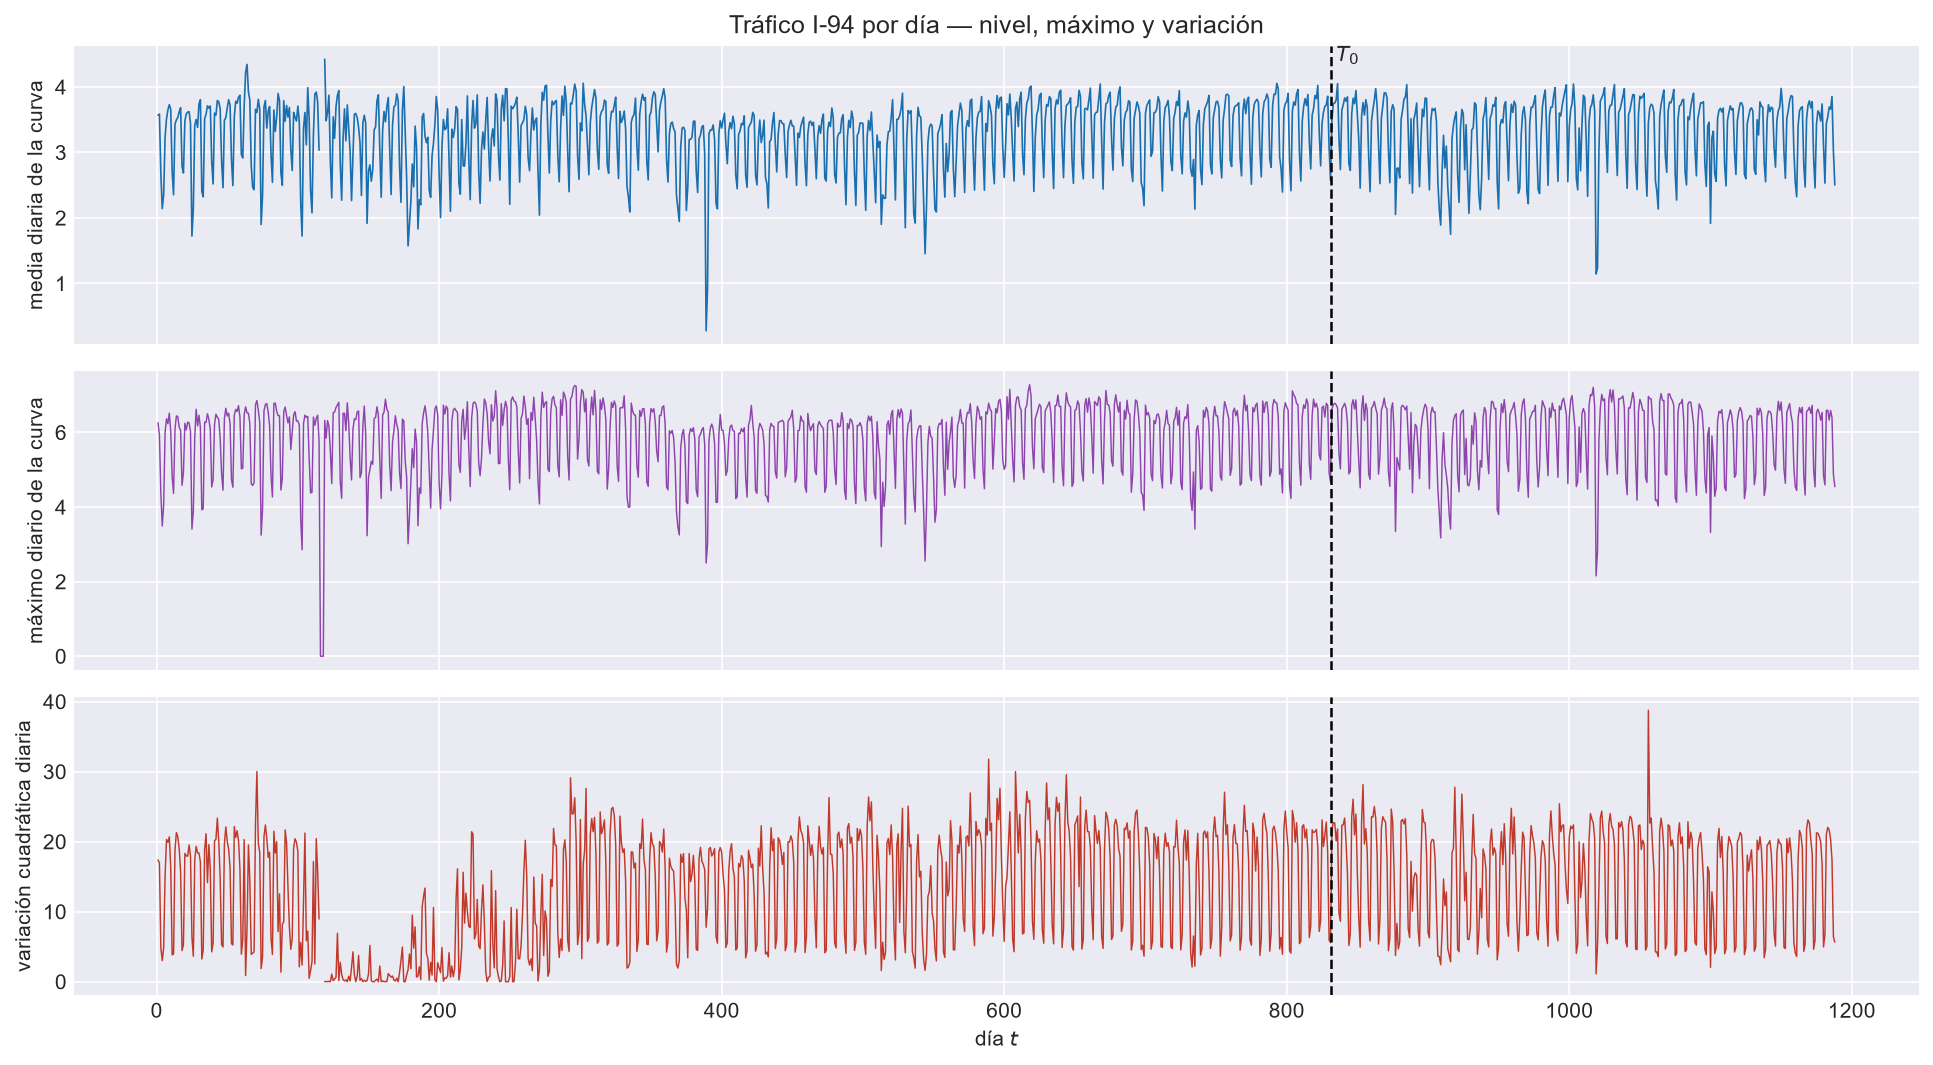
\includegraphics[width=\textwidth,height=0.7\textheight,keepaspectratio]{IMG/aneC_00/aneC_00_04_serie_diaria.png}
\caption{Serie diaria del volumen de tráfico.}
\label{fig:aneC_04_serie_diaria}
\end{figure}

\begin{figure}[H]
\centering
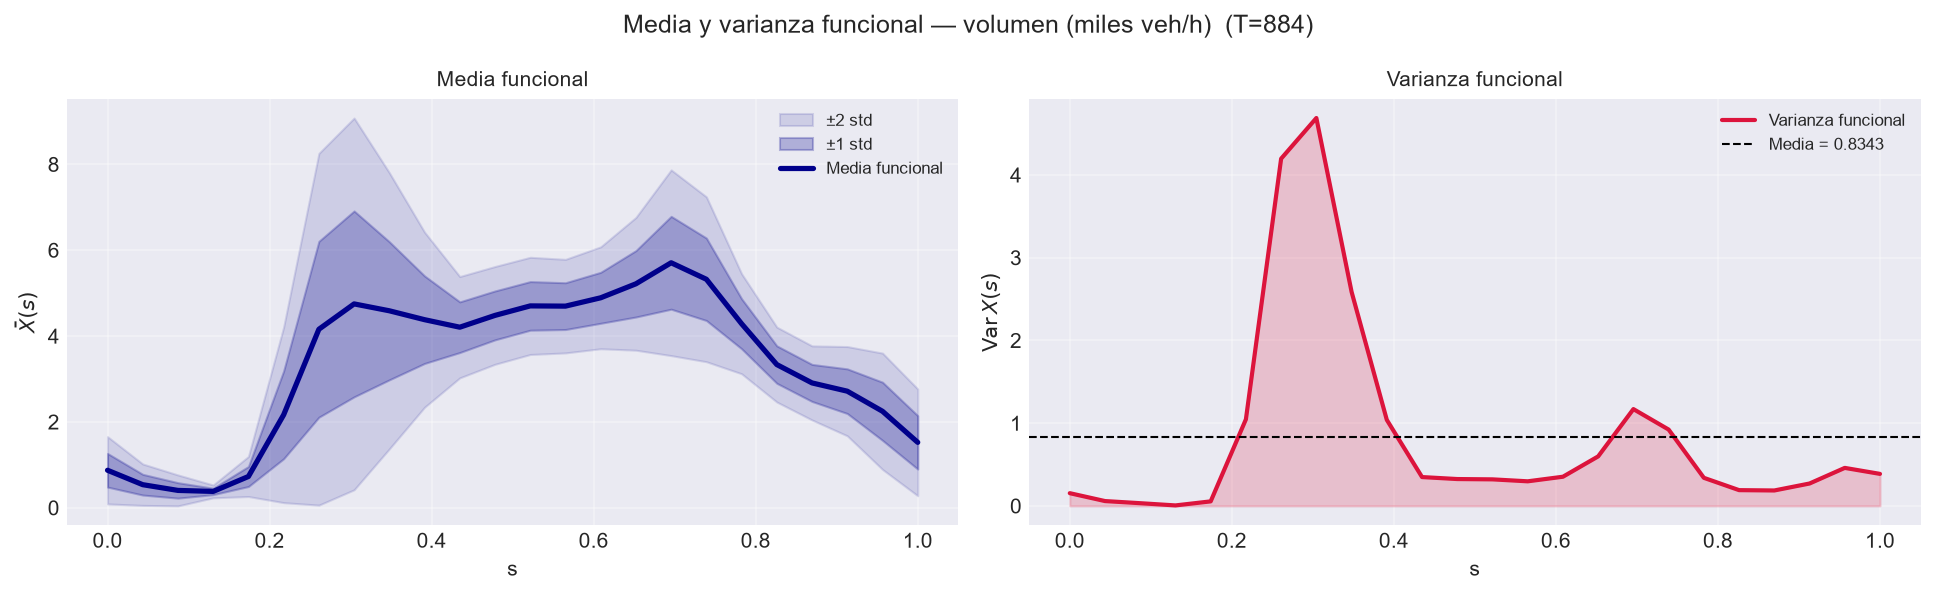
\includegraphics[width=\textwidth,height=0.7\textheight,keepaspectratio]{IMG/aneC_00/aneC_00_03_media_varianza_raw.png}
\caption{Media y varianza de la curva diaria.}
\label{fig:aneC_03_media_varianza_raw}
\end{figure}

\begin{figure}[H]
\centering
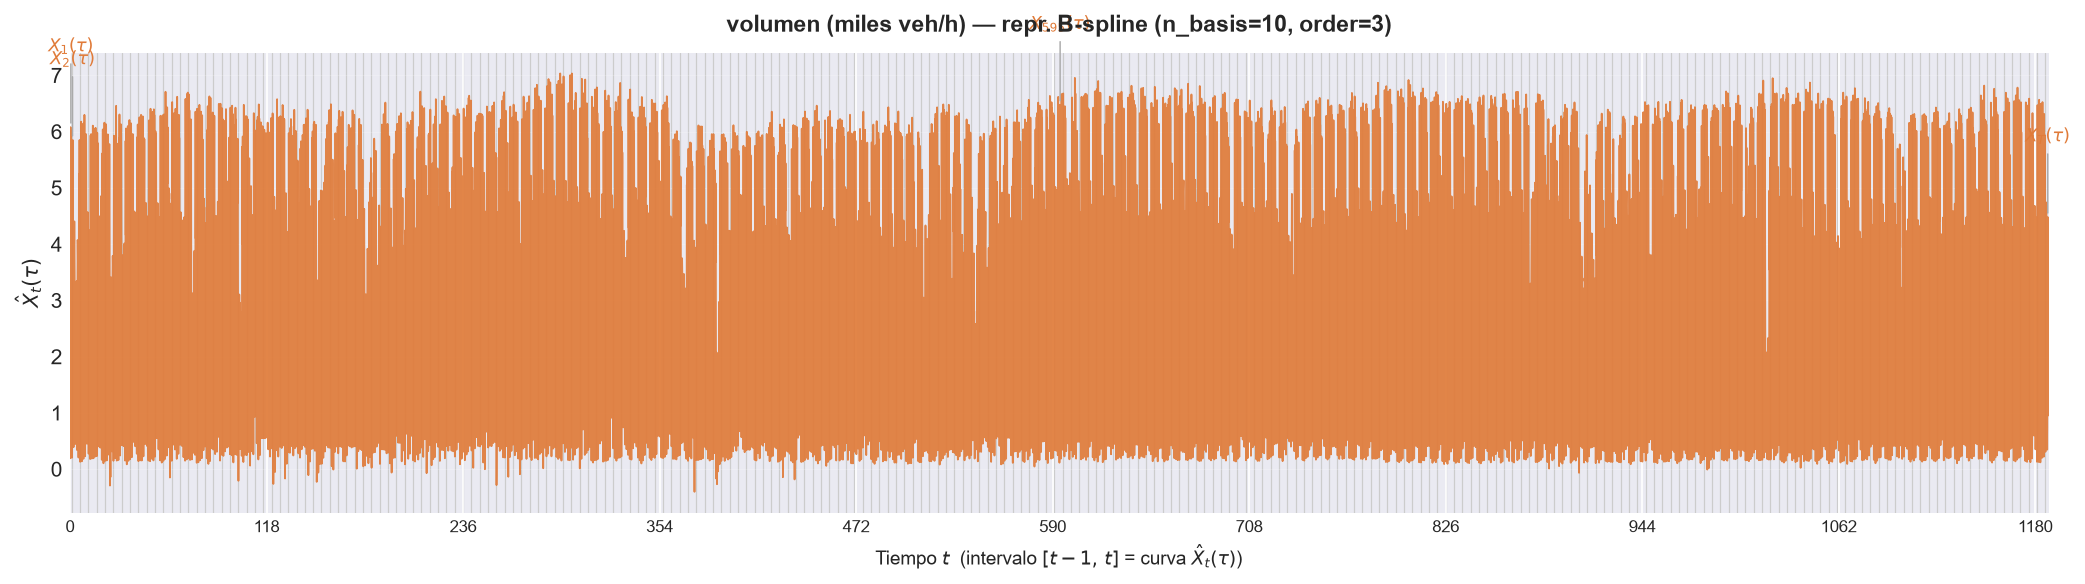
\includegraphics[width=\textwidth,height=0.7\textheight,keepaspectratio]{IMG/aneC_00/aneC_00_06_fts_funcional_bspline.png}
\caption{Curvas diarias en la base B-spline 10/3.}
\label{fig:aneC_06_fts_funcional_bspline}
\end{figure}

\begin{figure}[H]
\centering
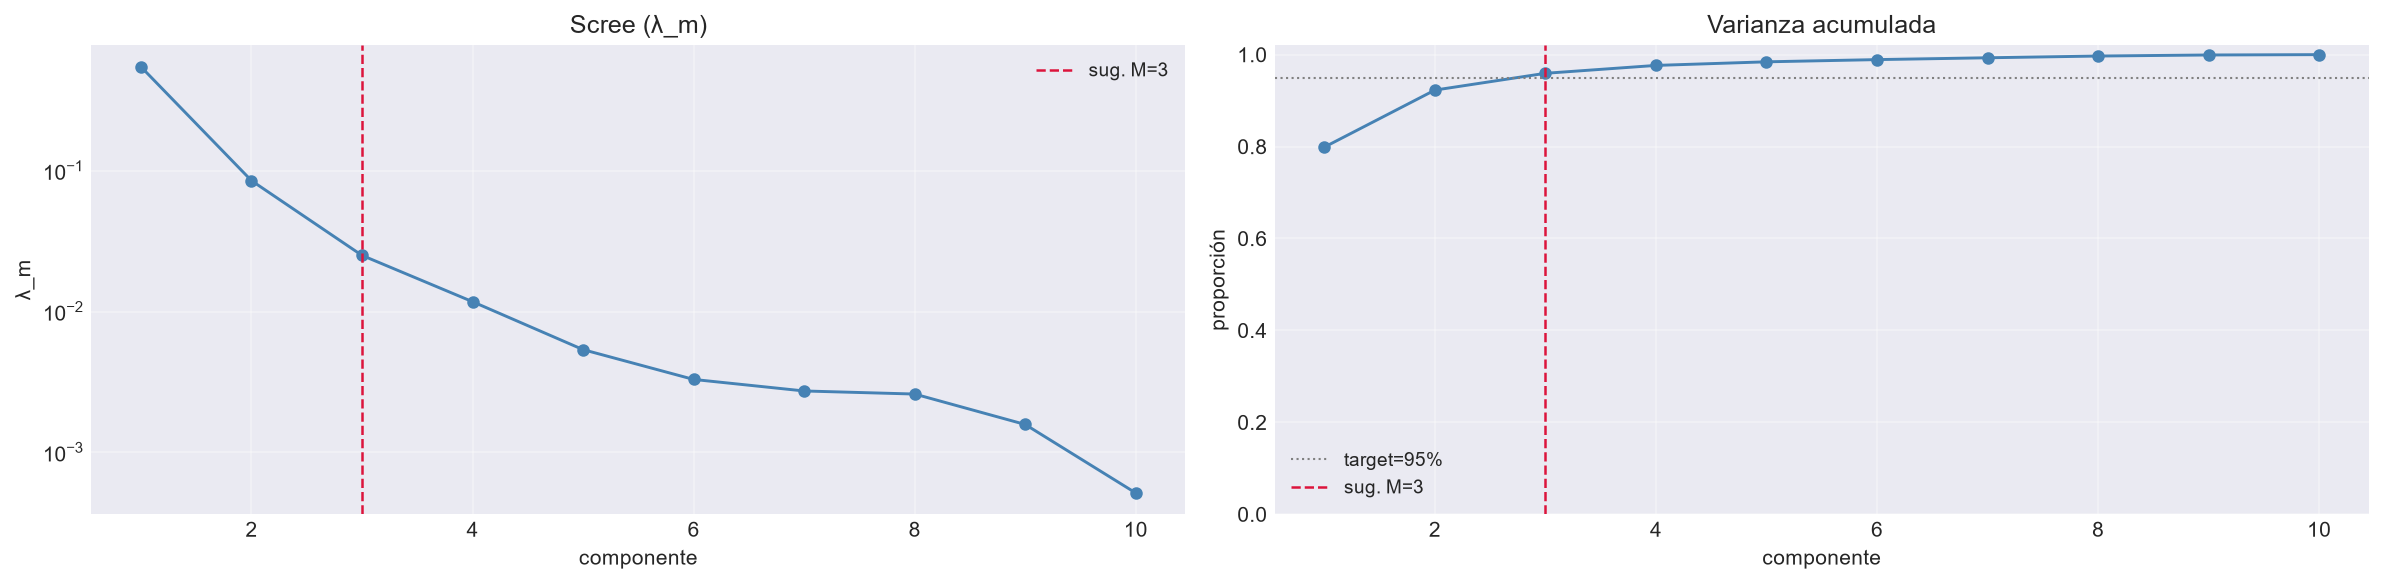
\includegraphics[width=\textwidth,height=0.7\textheight,keepaspectratio]{IMG/aneC_00/aneC_00_07_fpca_scree.png}
\caption{Varianza explicada por componente de la FPCA (train).}
\label{fig:aneC_07_fpca_scree}
\end{figure}

\begin{figure}[H]
\centering
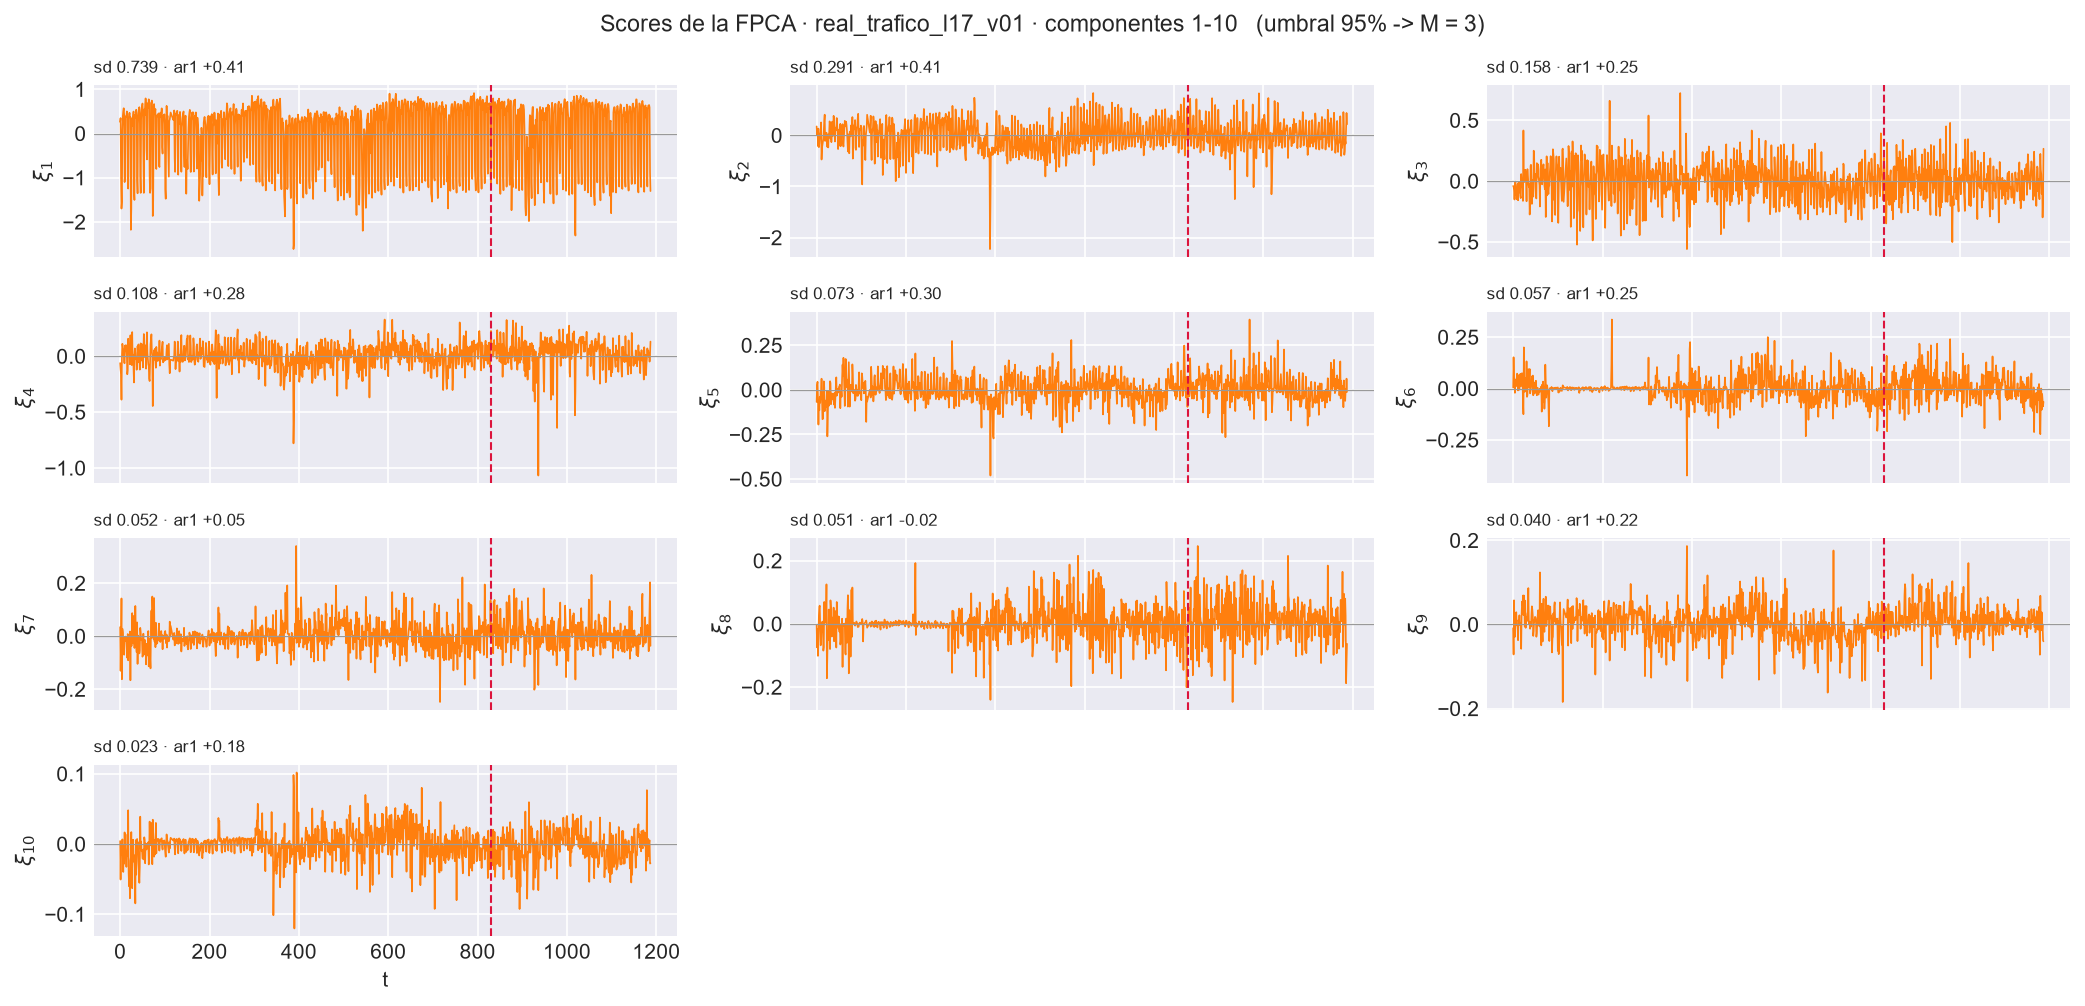
\includegraphics[width=\textwidth,height=0.7\textheight,keepaspectratio]{IMG/aneC_00/aneC_00_07b_series_scores.png}
\caption{Series de scores de la FPCA.}
\label{fig:aneC_07b_series_scores}
\end{figure}

\begin{figure}[H]
\centering
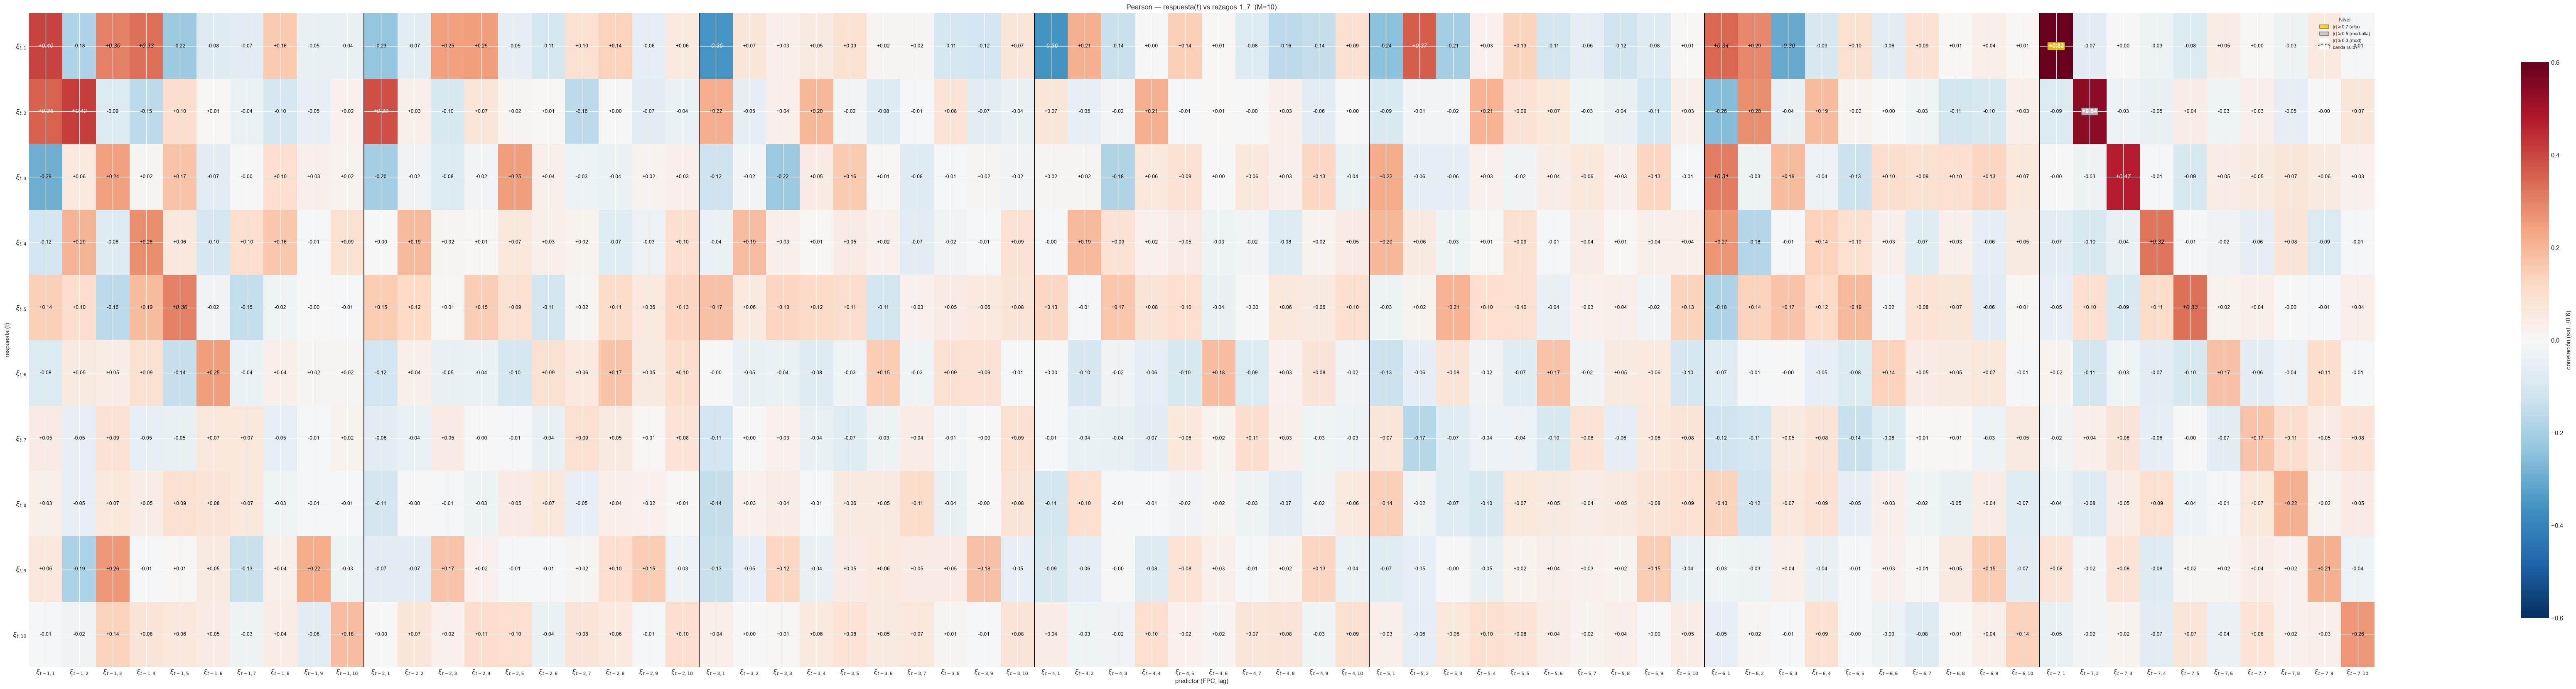
\includegraphics[width=\textwidth,height=0.7\textheight,keepaspectratio]{IMG/aneC_00/aneC_00_09a_rezagos_pearson.png}
\caption{Autocorrelación de los scores por rezago (Pearson).}
\label{fig:aneC_09a_rezagos_pearson}
\end{figure}

\begin{figure}[H]
\centering
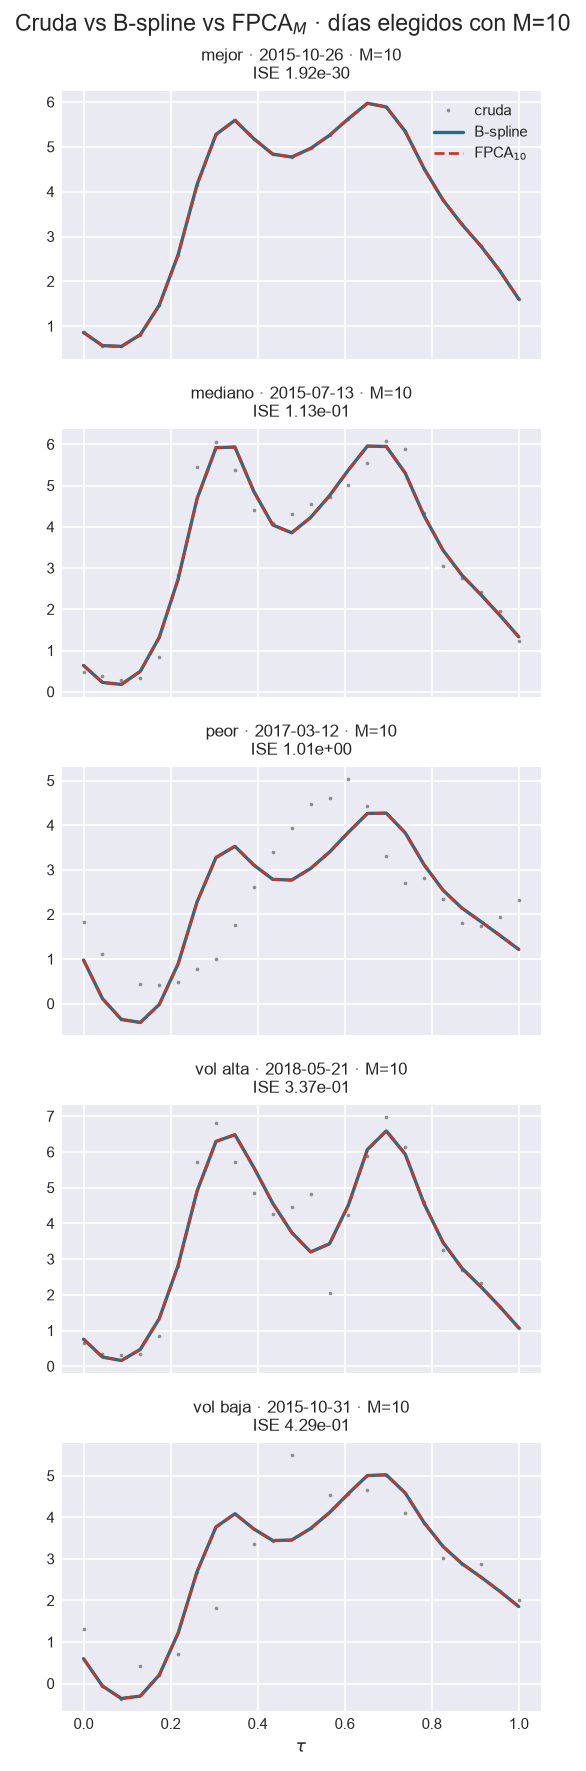
\includegraphics[width=\textwidth,height=0.7\textheight,keepaspectratio]{IMG/aneC_00/aneC_00_10_tres_curvas.png}
\caption{Tres curvas observadas y su representación con $M = 10$.}
\label{fig:aneC_10_tres_curvas}
\end{figure}

\section{Sensibilidad al ancho de la ventana}
\label{aneC_00_02_ventana}
% 58 y 59 con w = 20 y w = 40 (w = 30 está en el Capítulo 4).

\begin{figure}[H]
\centering
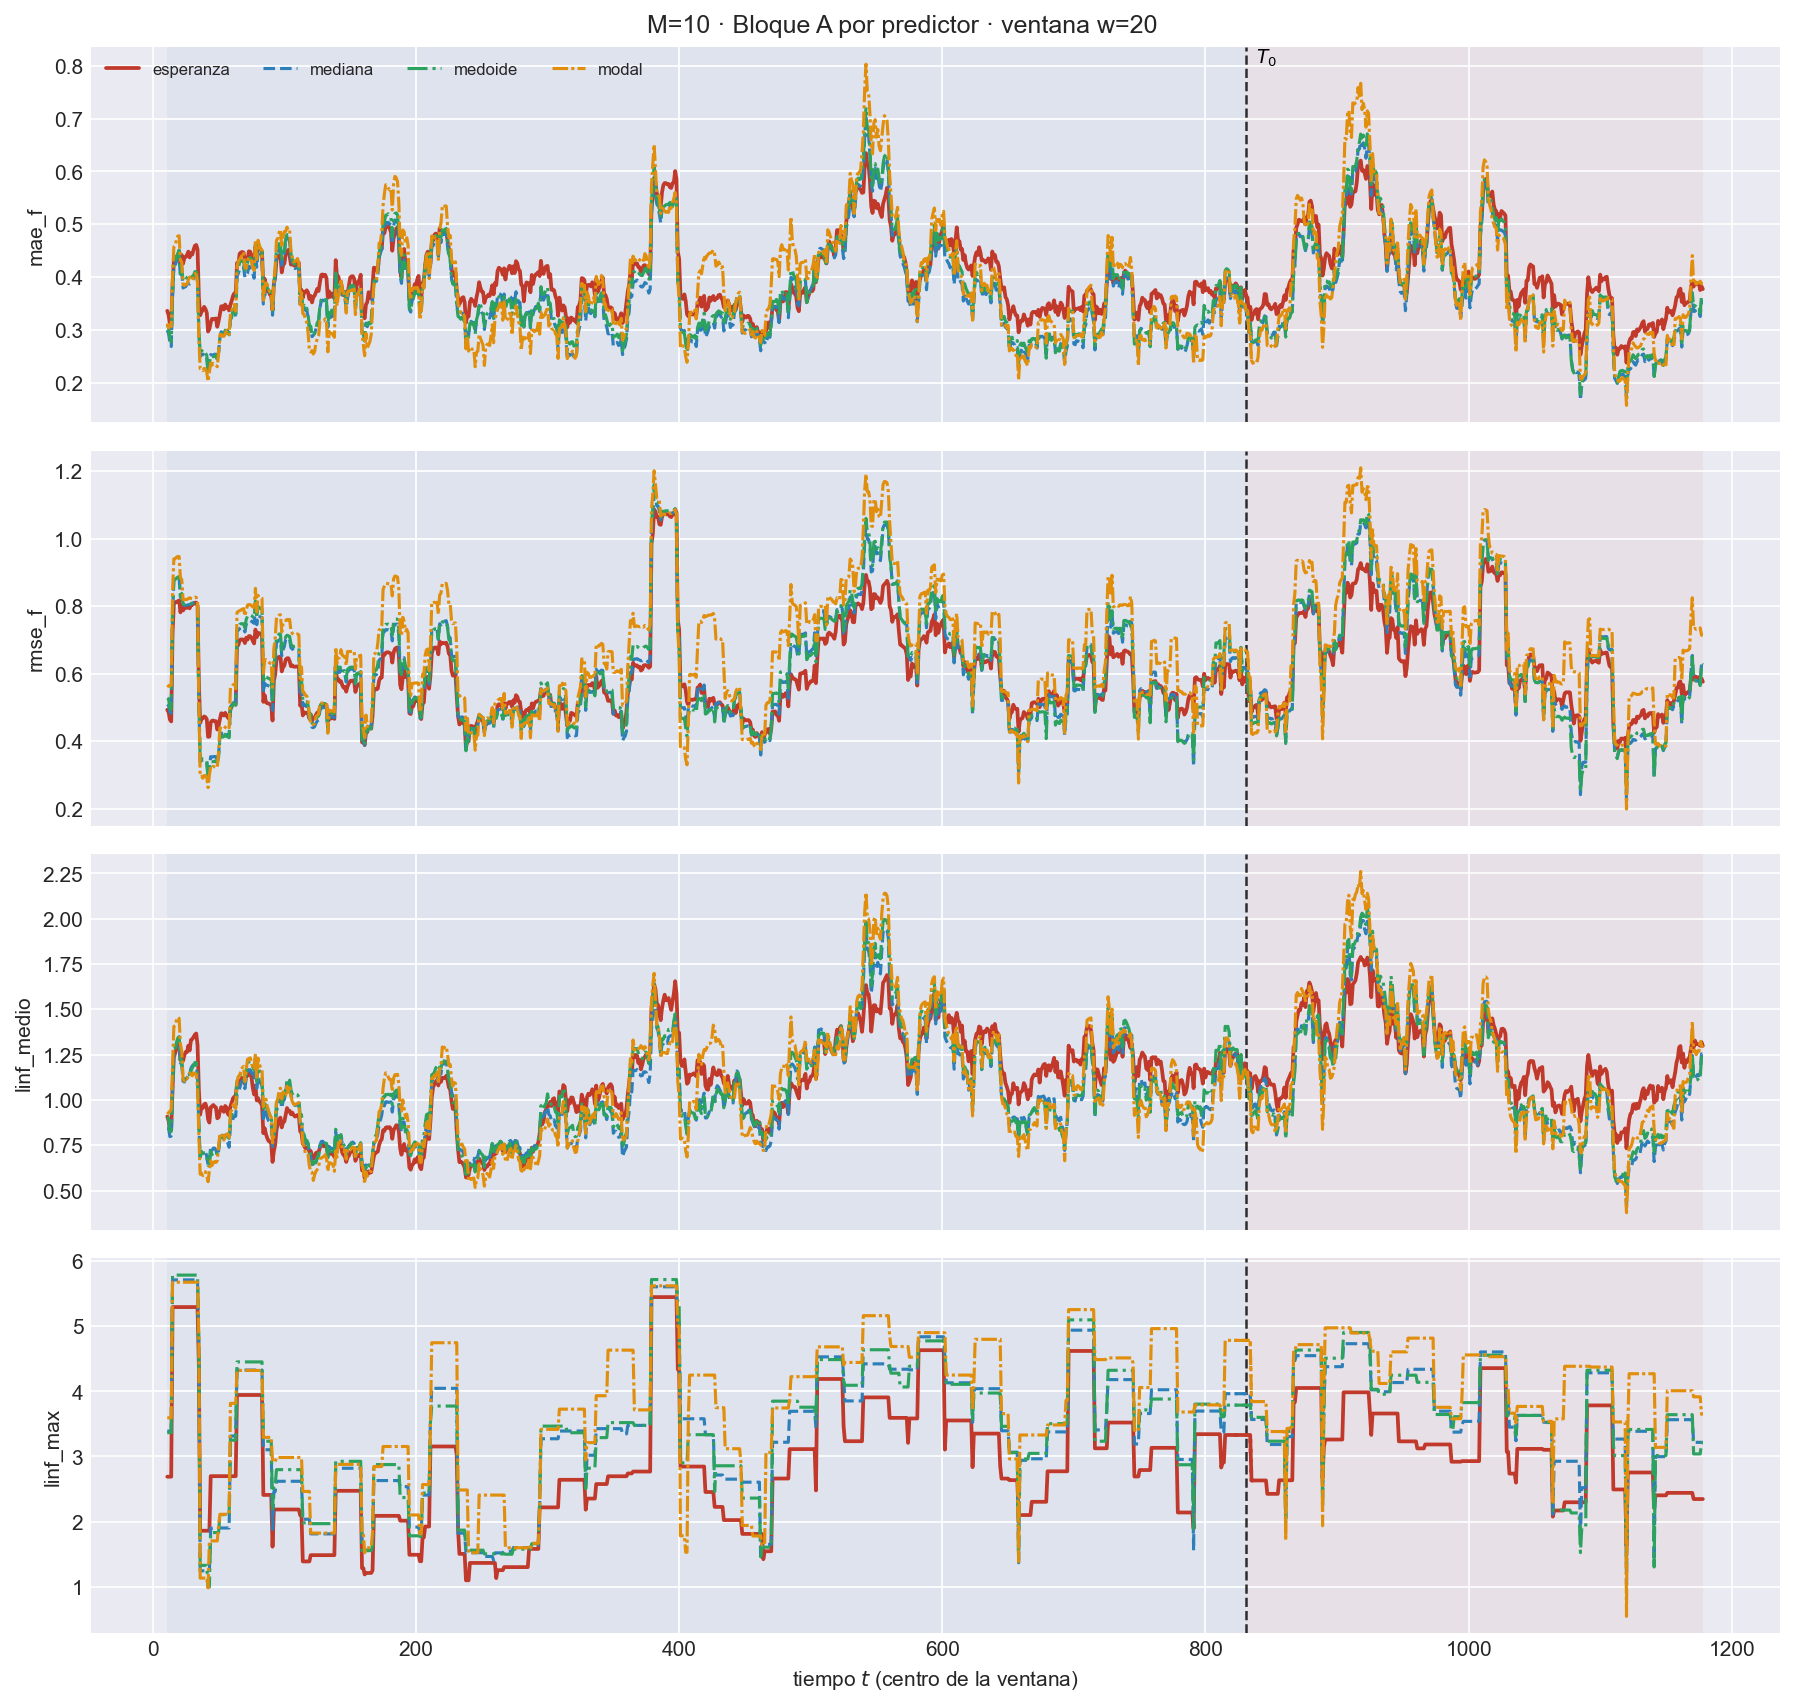
\includegraphics[width=\textwidth,height=0.7\textheight,keepaspectratio]{IMG/aneC_00/aneC_00_58_ventana_predictores_w20_101.png}
\caption{Ventana móvil $w = 20$: predictores puntuales, tráfico $\{1\}$ ($M = 10$).}
\label{fig:aneC_58_ventana_predictores_w20_101}
\end{figure}

\begin{figure}[H]
\centering
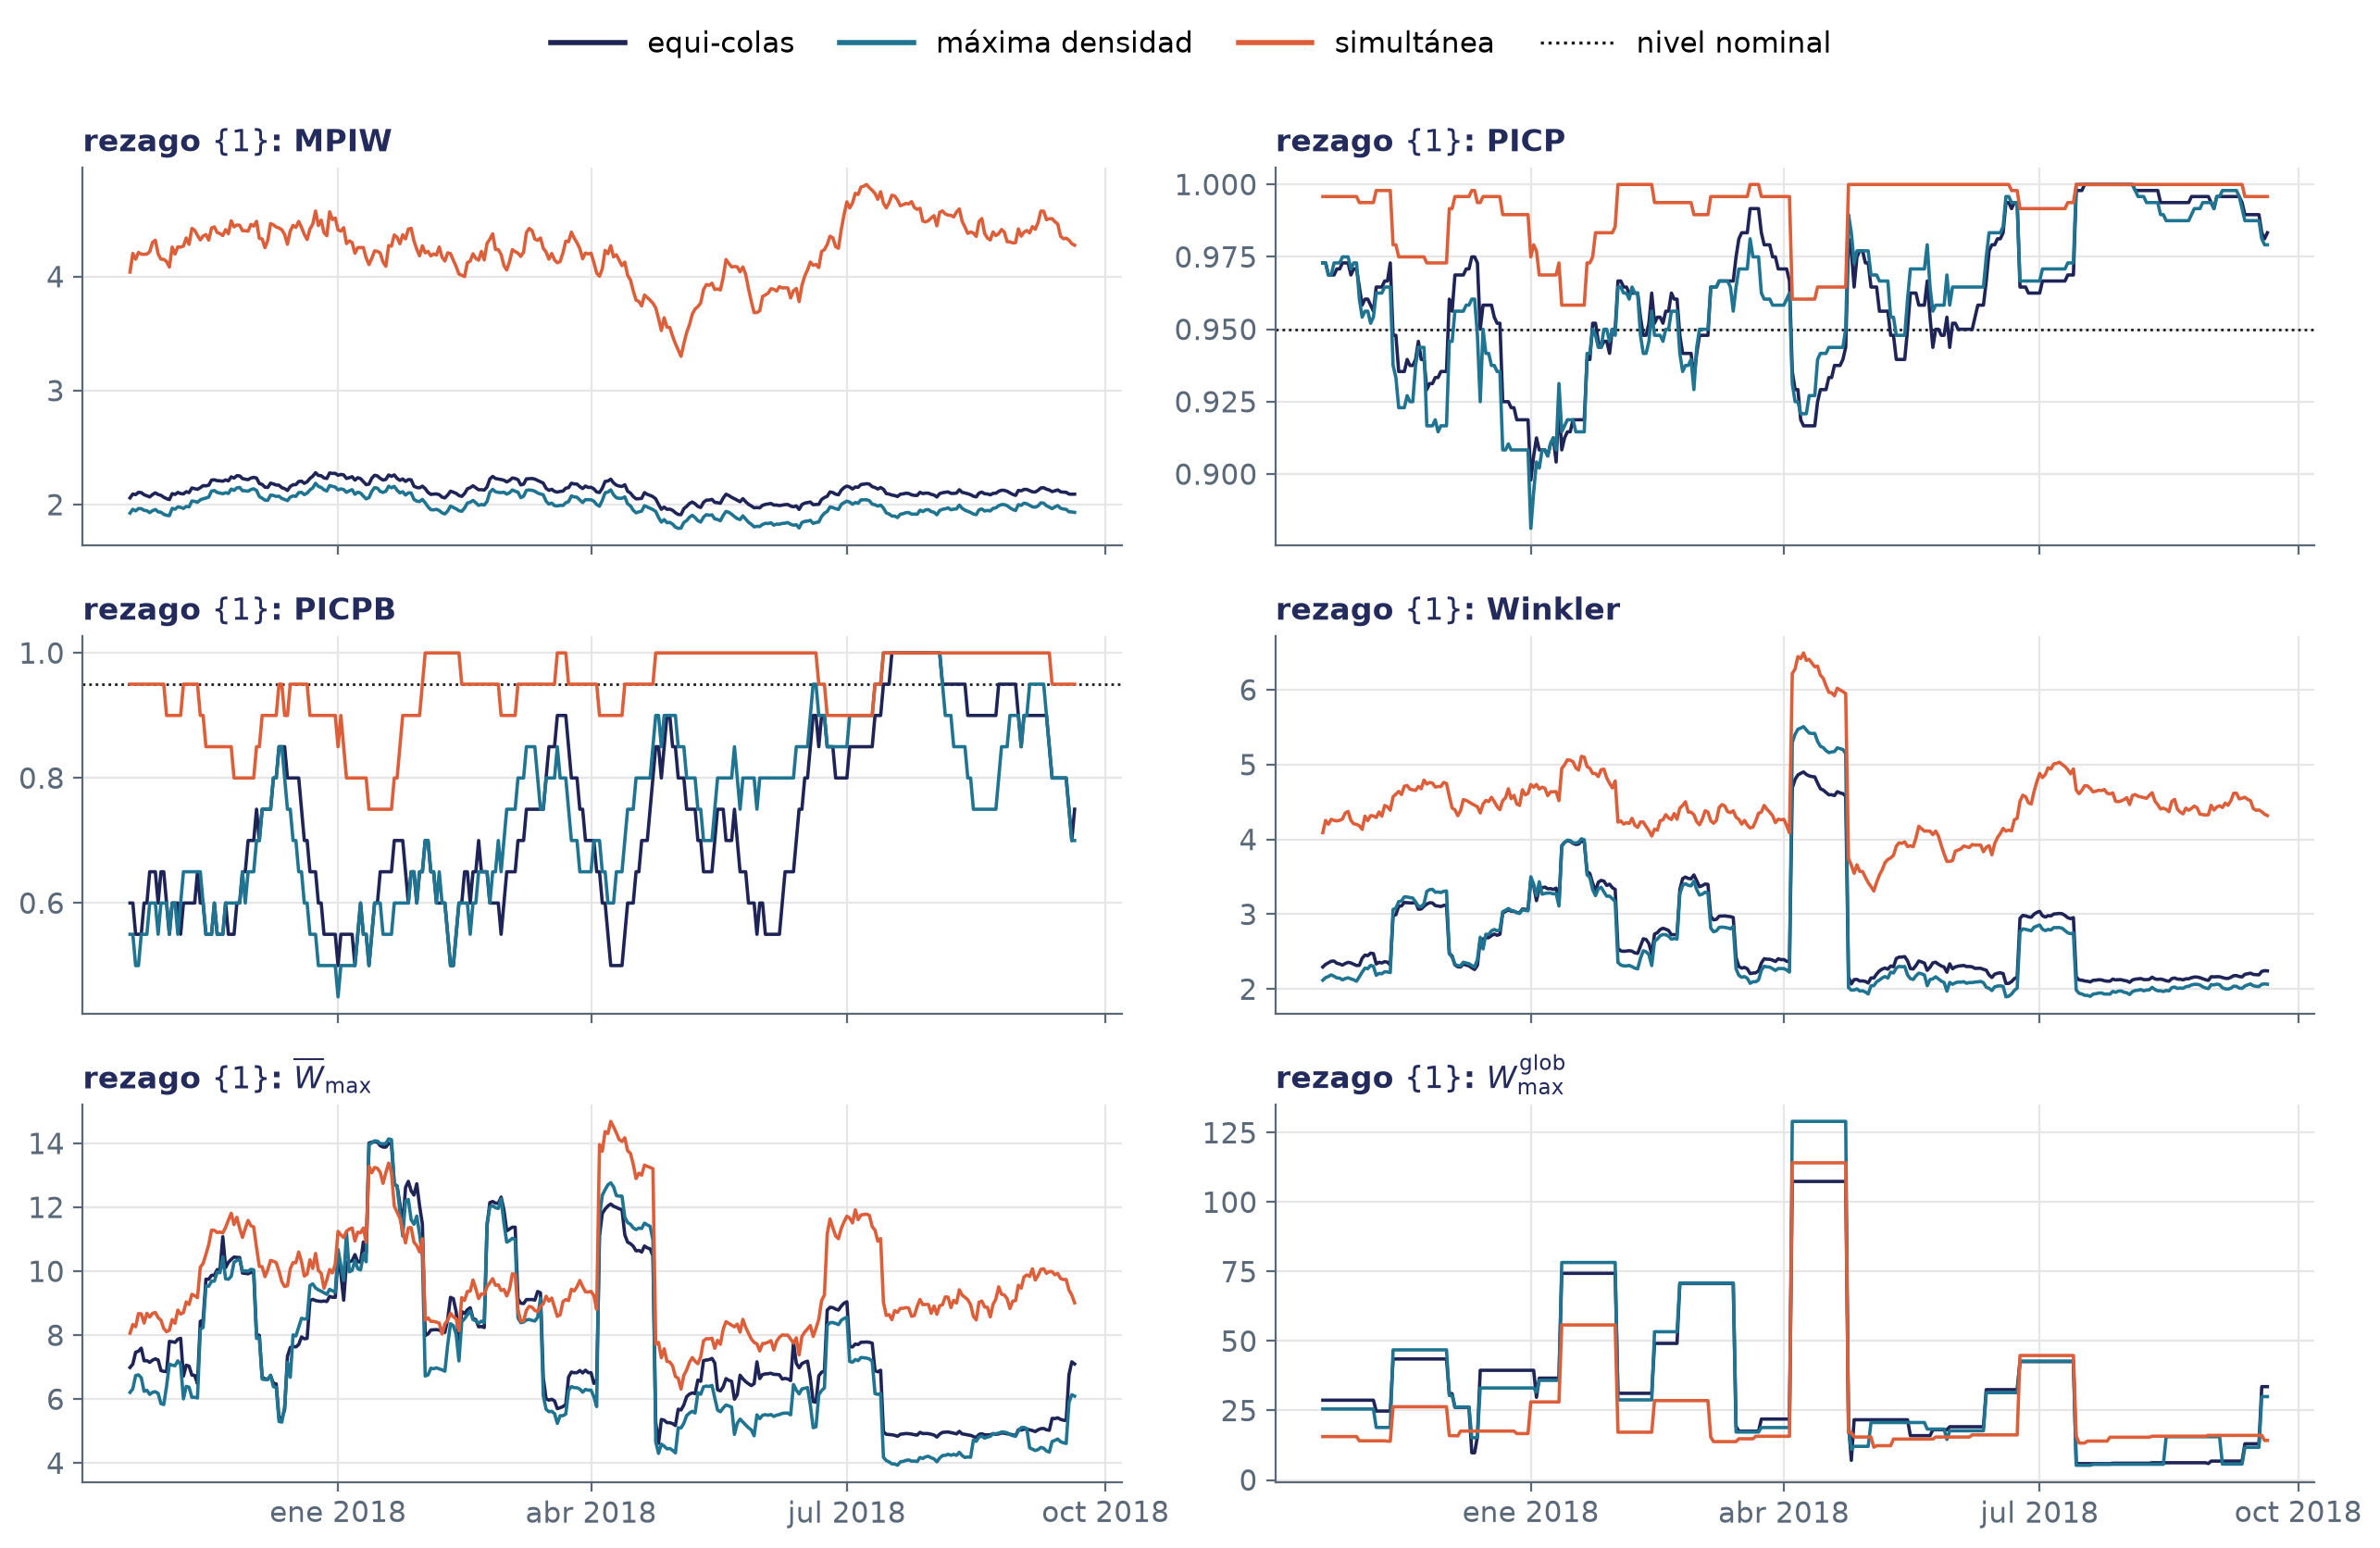
\includegraphics[width=\textwidth,height=0.7\textheight,keepaspectratio]{IMG/aneC_00/aneC_00_59_ventana_intervalos_w20_101.png}
\caption{Ventana móvil $w = 20$: intervalos, tráfico $\{1\}$ ($M = 10$).}
\label{fig:aneC_59_ventana_intervalos_w20_101}
\end{figure}

\begin{figure}[H]
\centering
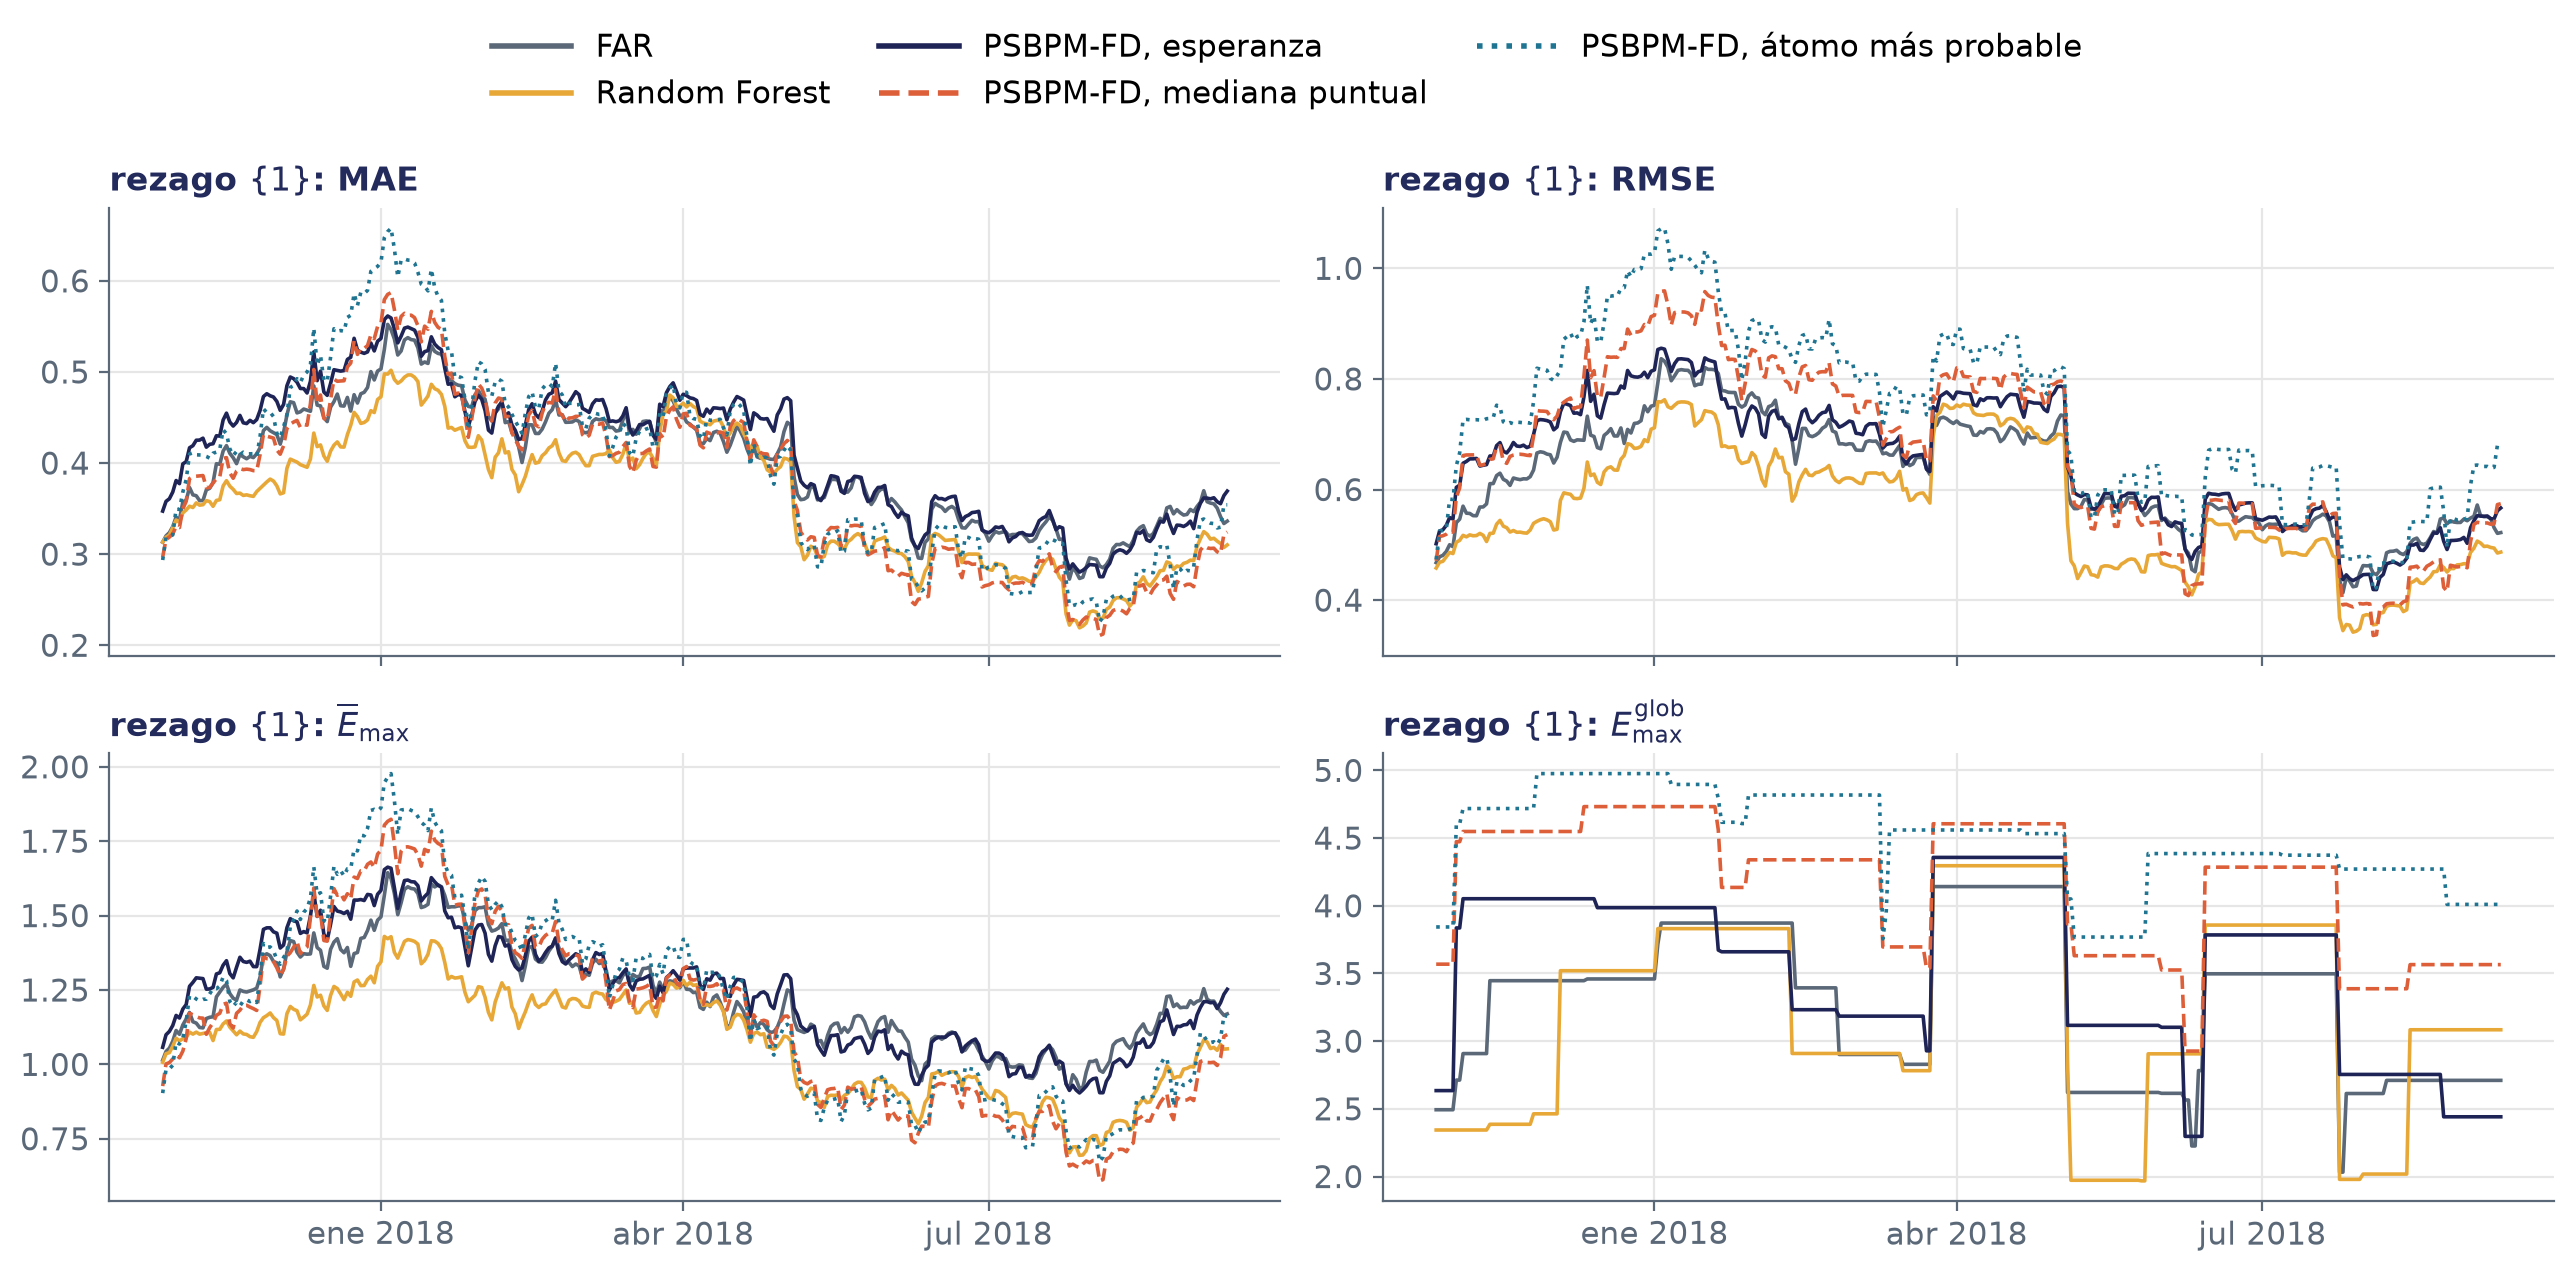
\includegraphics[width=\textwidth,height=0.7\textheight,keepaspectratio]{IMG/aneC_00/aneC_00_58_ventana_predictores_w40_101.png}
\caption{Ventana móvil $w = 40$: predictores puntuales, tráfico $\{1\}$ ($M = 10$).}
\label{fig:aneC_58_ventana_predictores_w40_101}
\end{figure}

\begin{figure}[H]
\centering
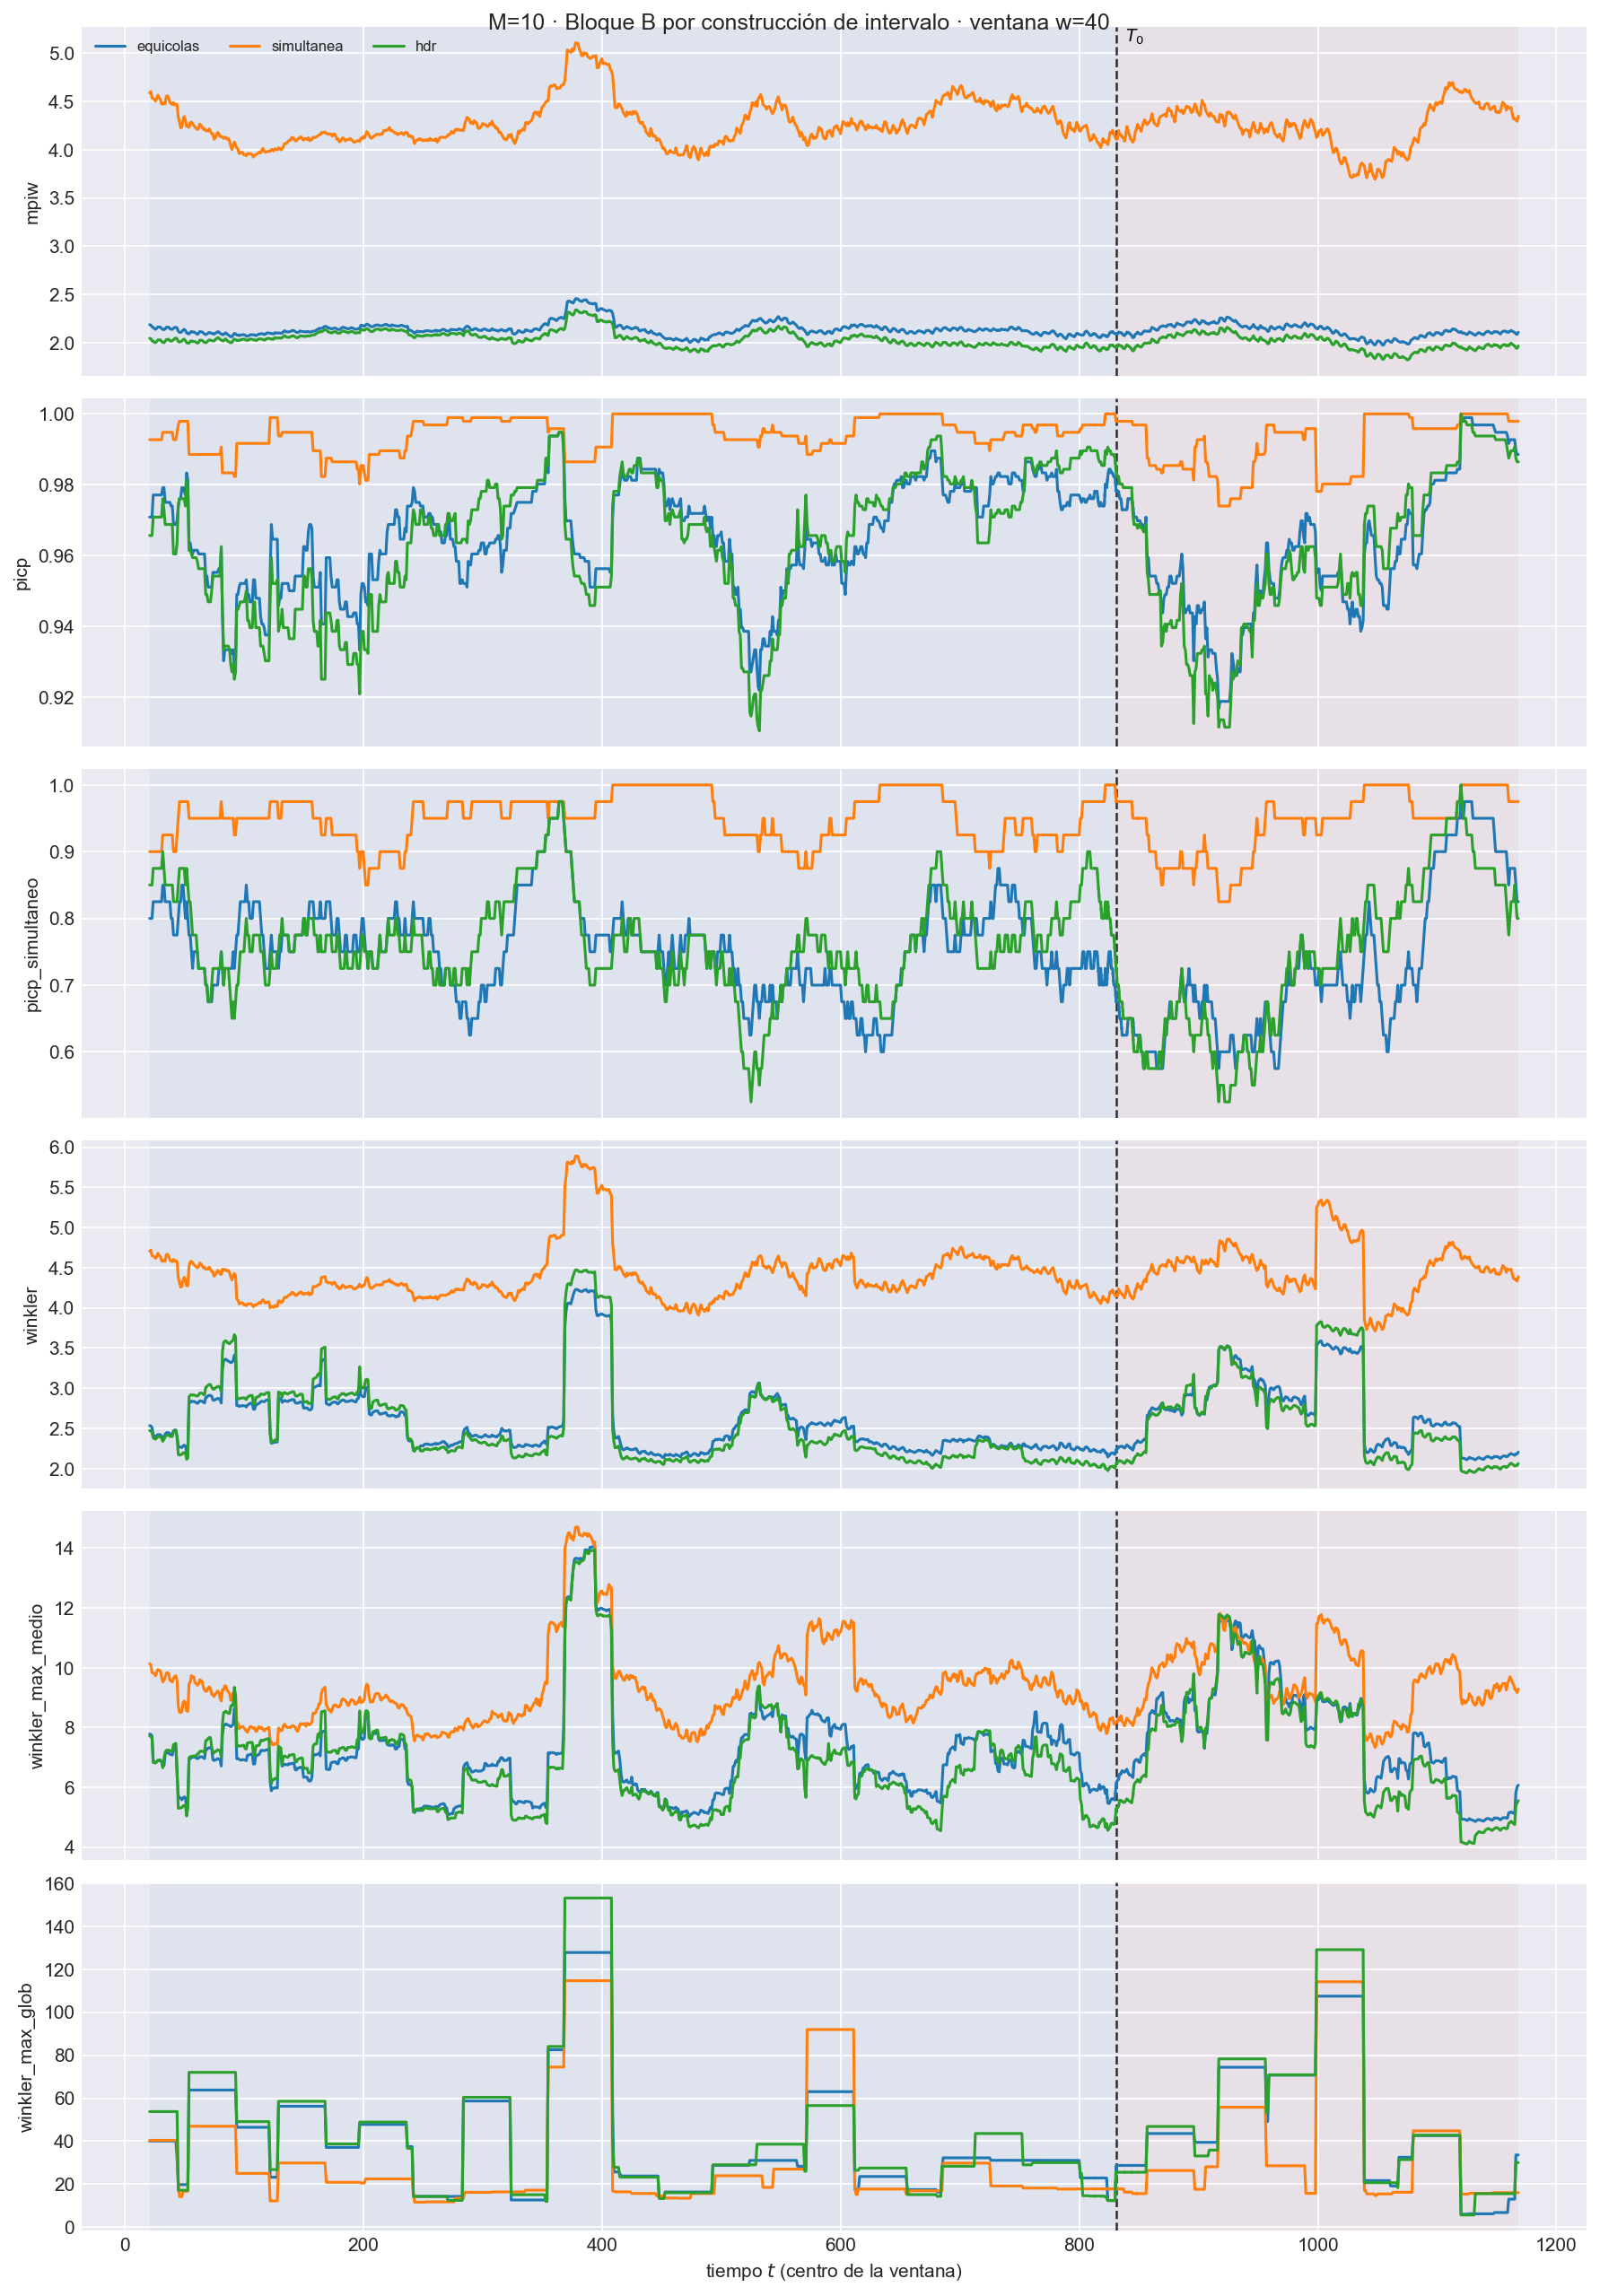
\includegraphics[width=\textwidth,height=0.7\textheight,keepaspectratio]{IMG/aneC_00/aneC_00_59_ventana_intervalos_w40_101.png}
\caption{Ventana móvil $w = 40$: intervalos, tráfico $\{1\}$ ($M = 10$).}
\label{fig:aneC_59_ventana_intervalos_w40_101}
\end{figure}

\begin{figure}[H]
\centering
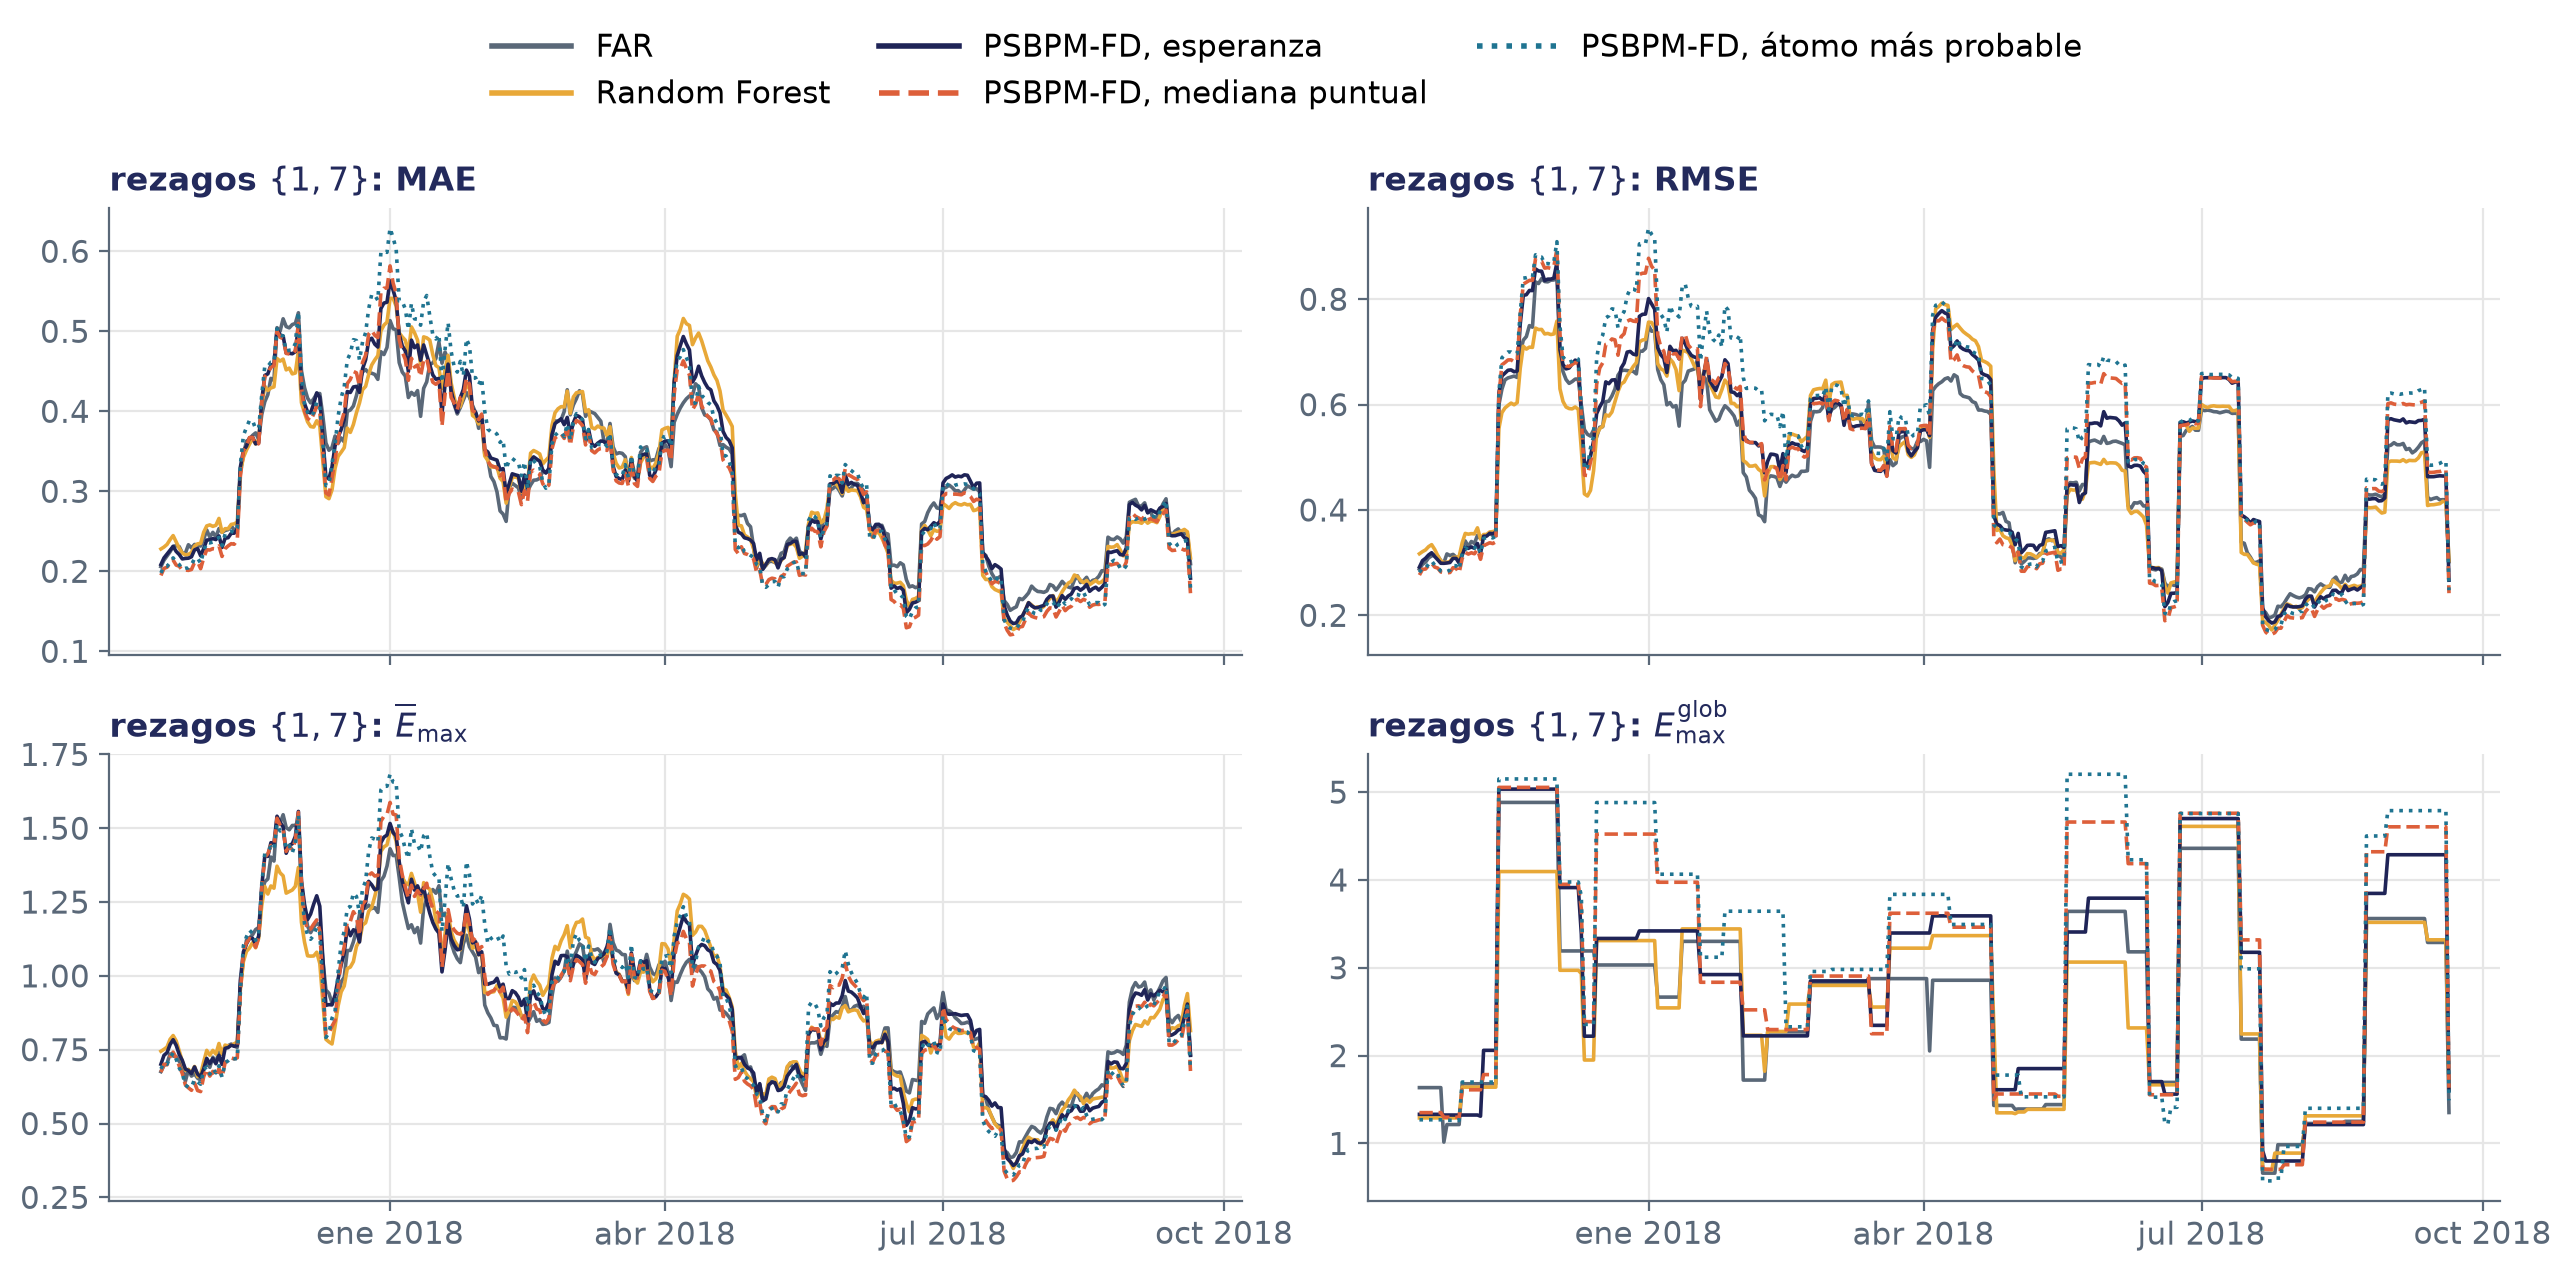
\includegraphics[width=\textwidth,height=0.7\textheight,keepaspectratio]{IMG/aneC_00/aneC_00_58_ventana_predictores_w20_102.png}
\caption{Ventana móvil $w = 20$: predictores puntuales, tráfico $\{1,7\}$ ($M = 10$).}
\label{fig:aneC_58_ventana_predictores_w20_102}
\end{figure}

\begin{figure}[H]
\centering
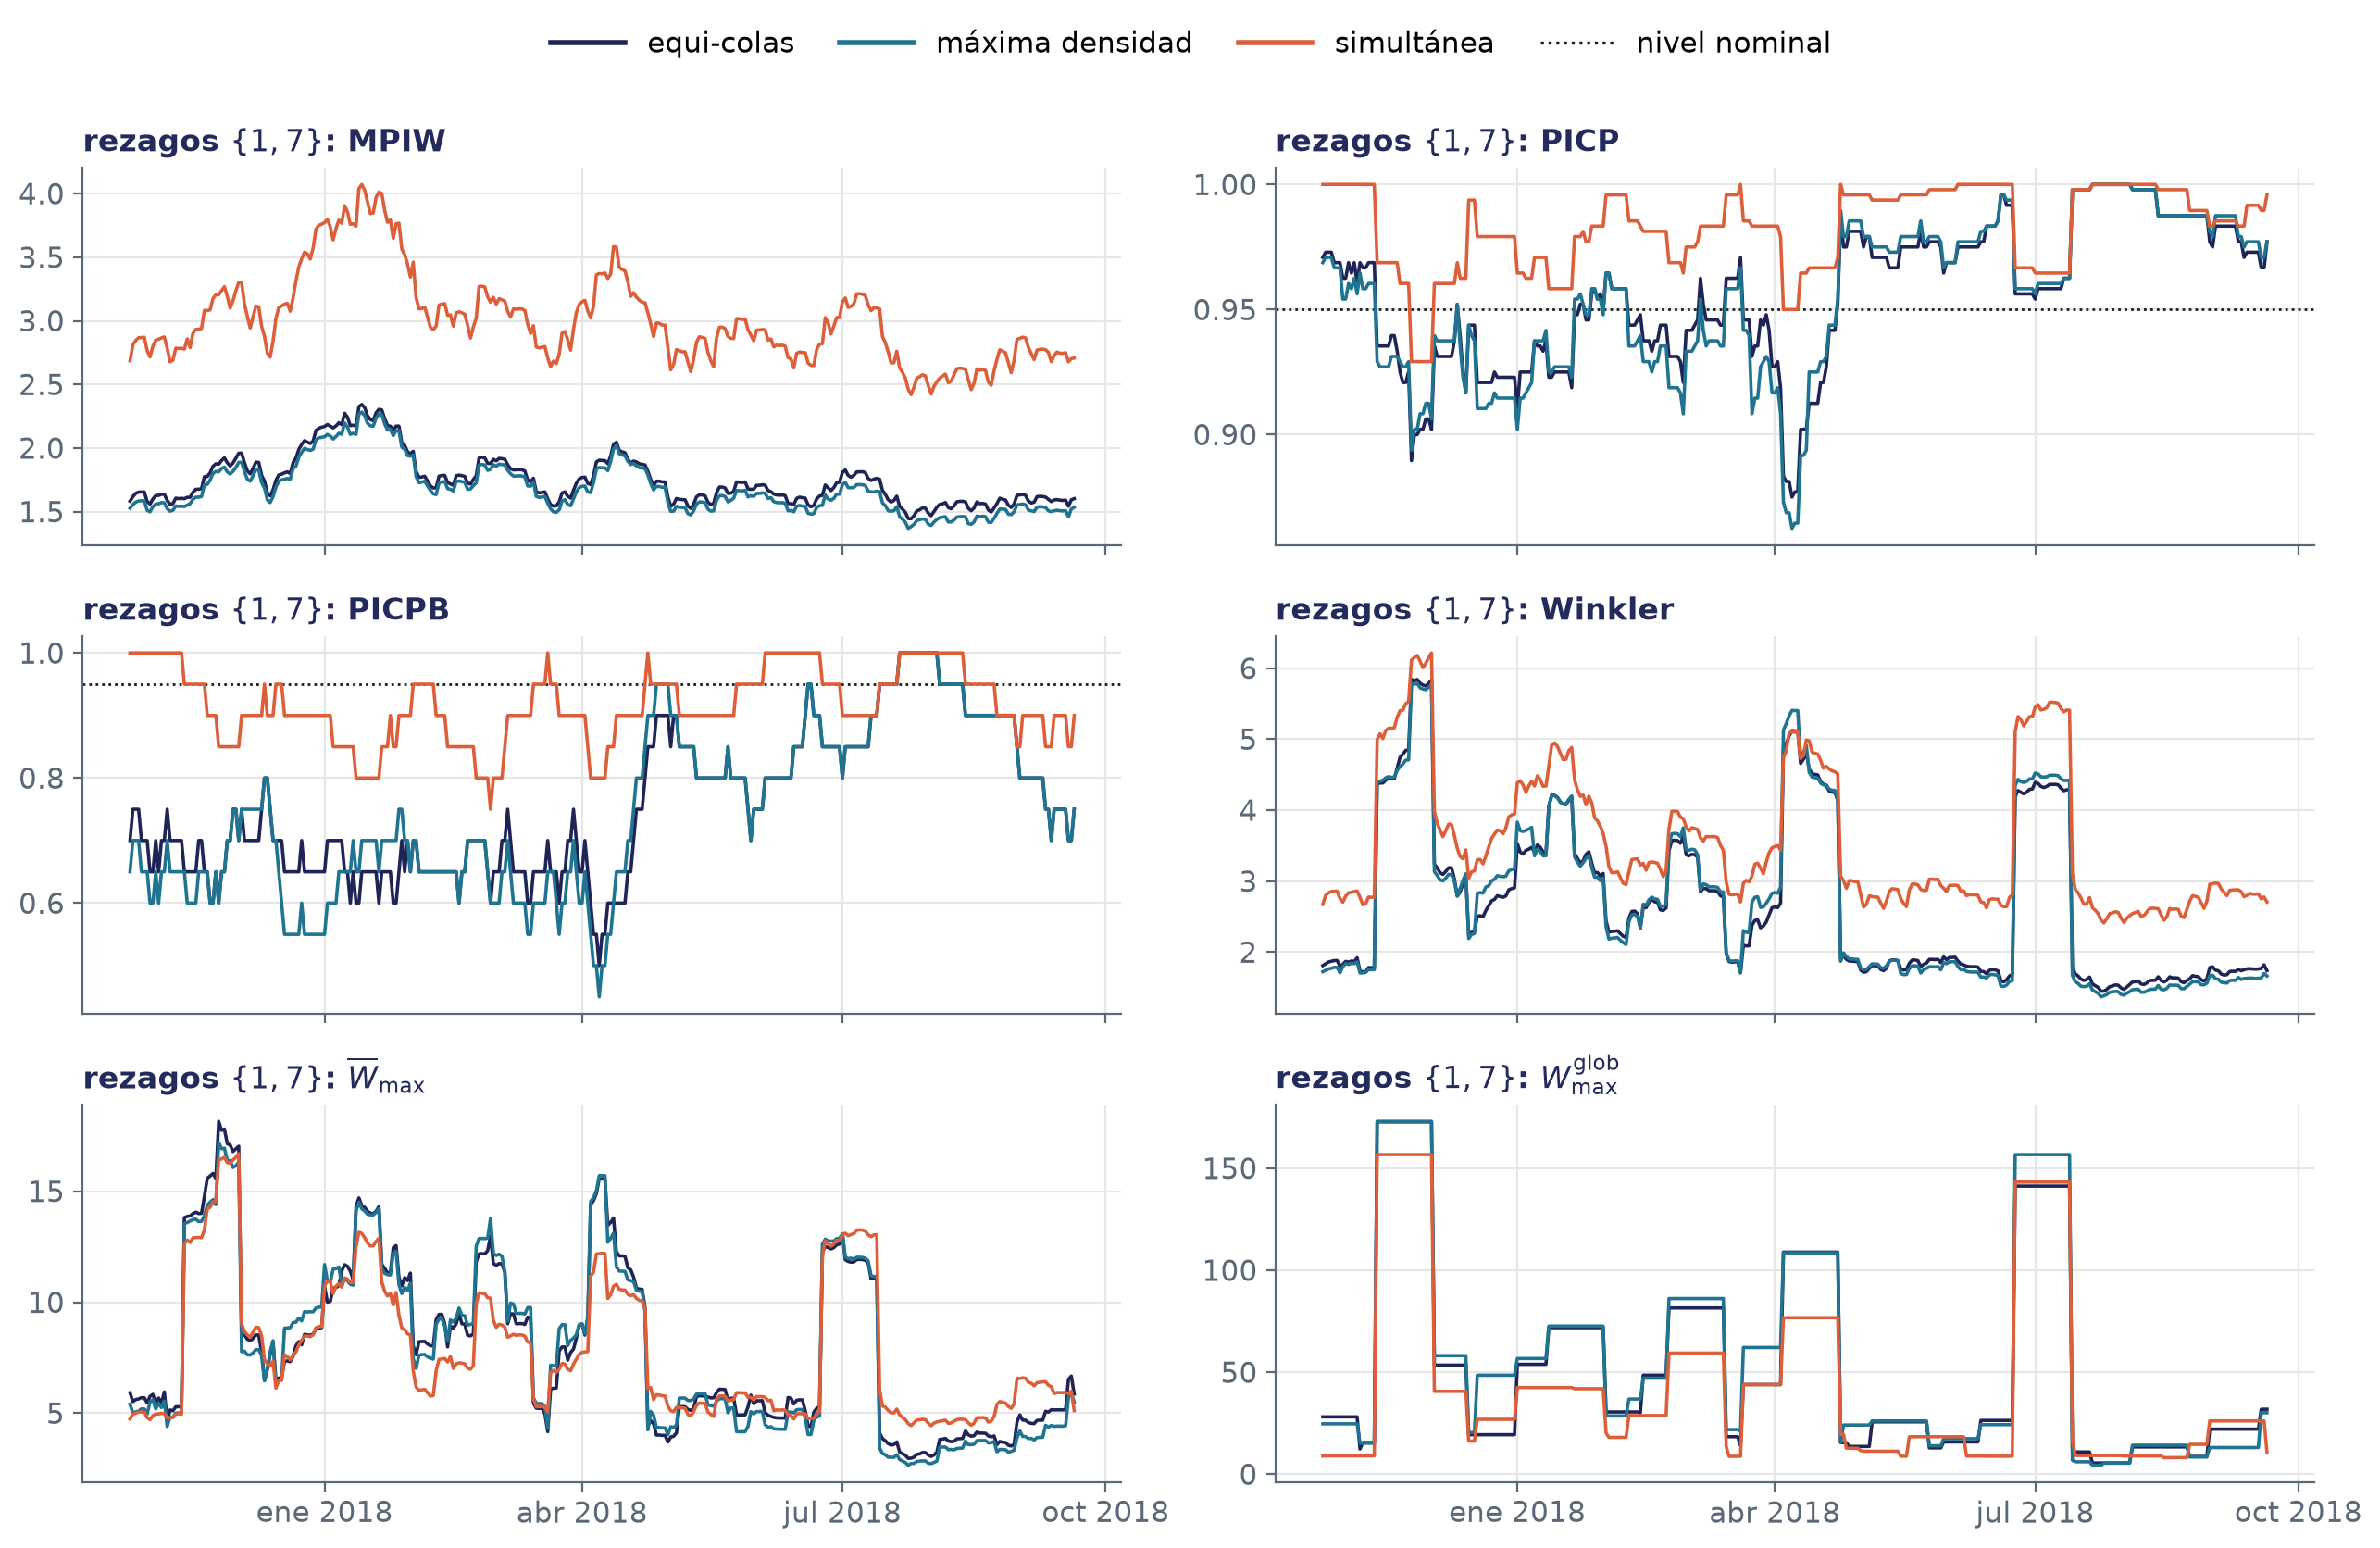
\includegraphics[width=\textwidth,height=0.7\textheight,keepaspectratio]{IMG/aneC_00/aneC_00_59_ventana_intervalos_w20_102.png}
\caption{Ventana móvil $w = 20$: intervalos, tráfico $\{1,7\}$ ($M = 10$).}
\label{fig:aneC_59_ventana_intervalos_w20_102}
\end{figure}

\begin{figure}[H]
\centering
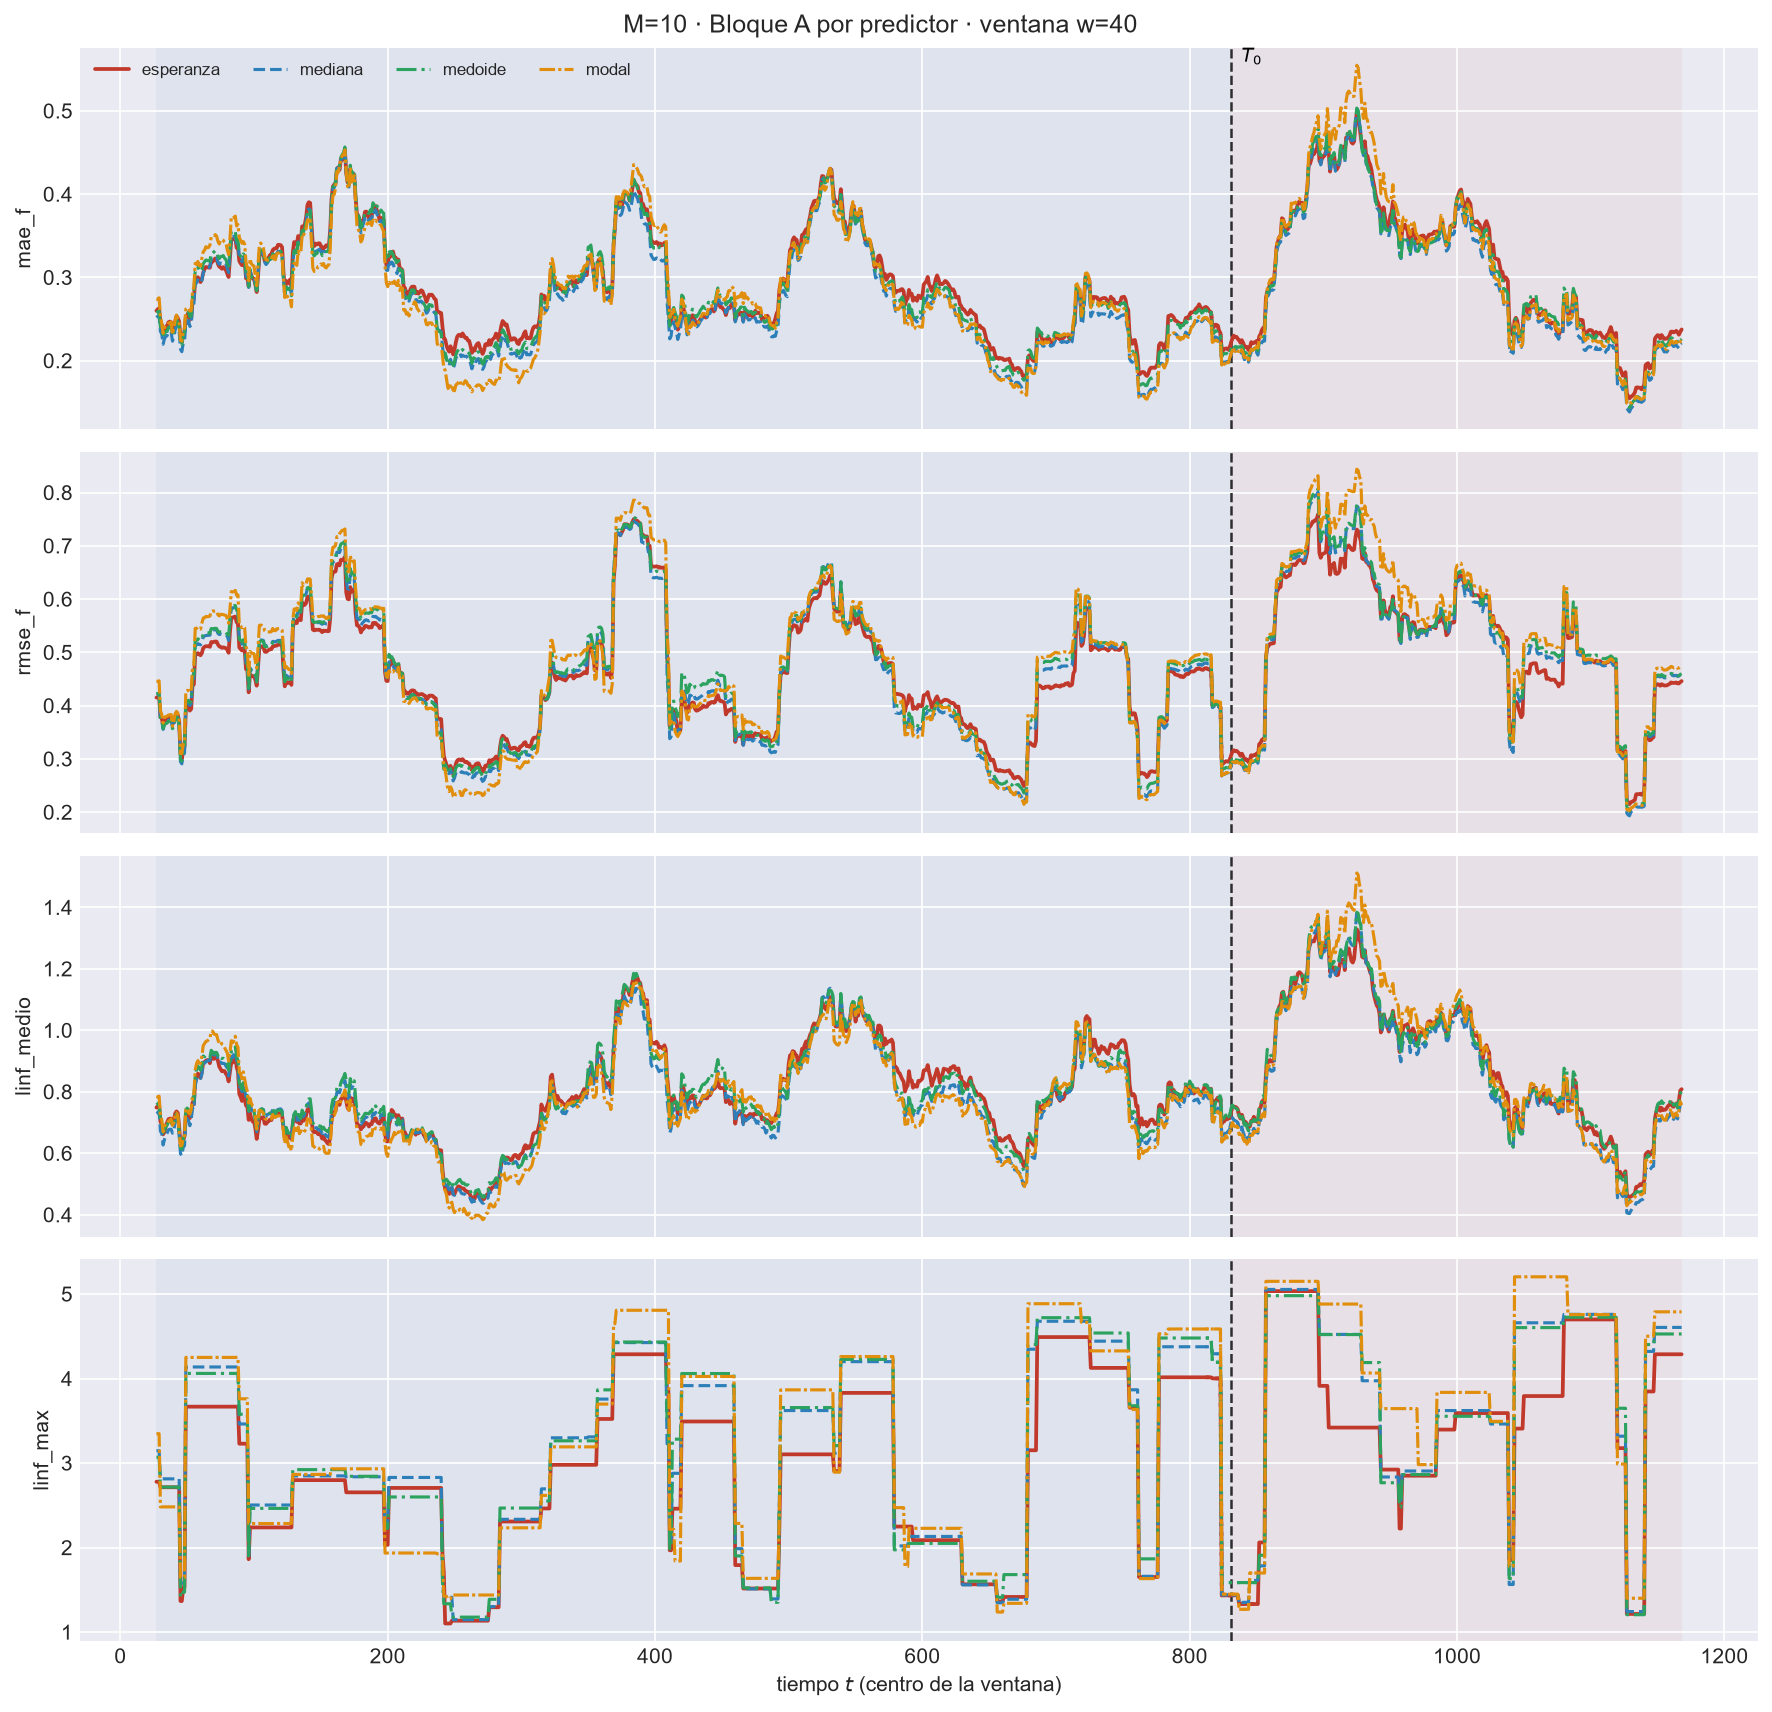
\includegraphics[width=\textwidth,height=0.7\textheight,keepaspectratio]{IMG/aneC_00/aneC_00_58_ventana_predictores_w40_102.png}
\caption{Ventana móvil $w = 40$: predictores puntuales, tráfico $\{1,7\}$ ($M = 10$).}
\label{fig:aneC_58_ventana_predictores_w40_102}
\end{figure}

\begin{figure}[H]
\centering
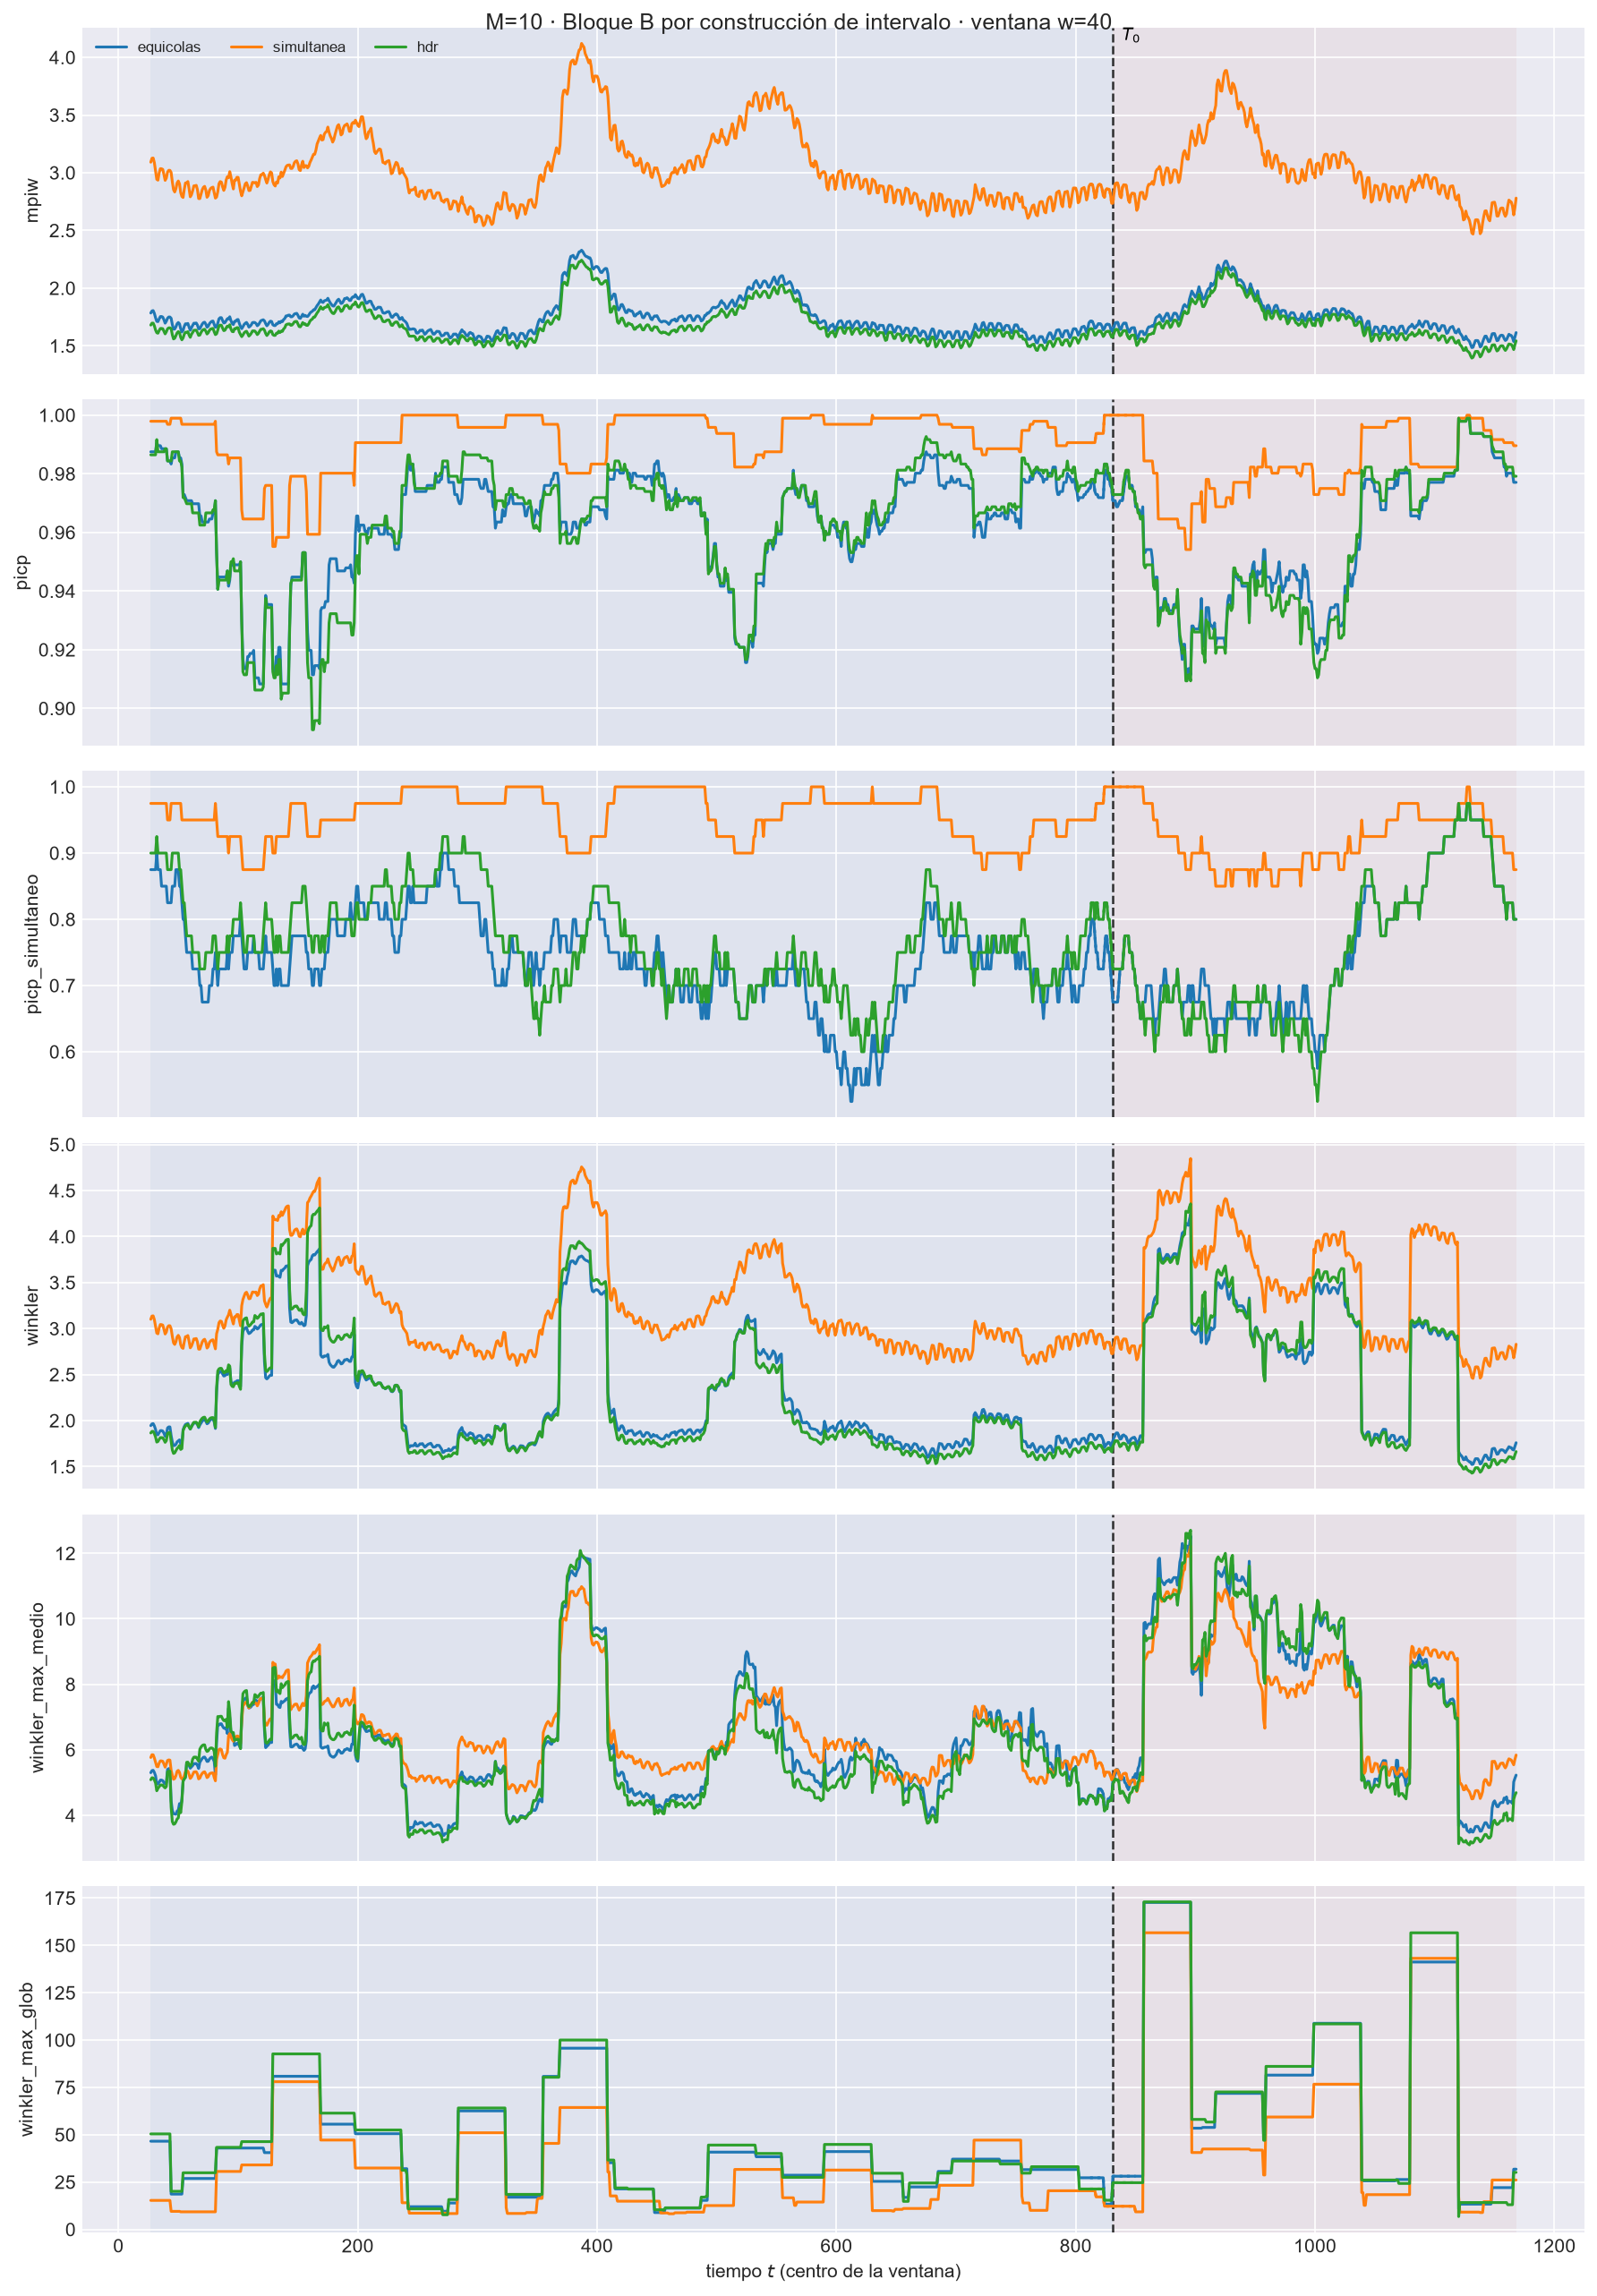
\includegraphics[width=\textwidth,height=0.7\textheight,keepaspectratio]{IMG/aneC_00/aneC_00_59_ventana_intervalos_w40_102.png}
\caption{Ventana móvil $w = 40$: intervalos, tráfico $\{1,7\}$ ($M = 10$).}
\label{fig:aneC_59_ventana_intervalos_w40_102}
\end{figure}

\section{Predicciones curva a curva}
\label{aneC_00_03_curvas}
% 54 y 55: extractos del bloque de prueba y de la frontera; 56b: el peor origen por RMSE.

\begin{figure}[H]
\centering
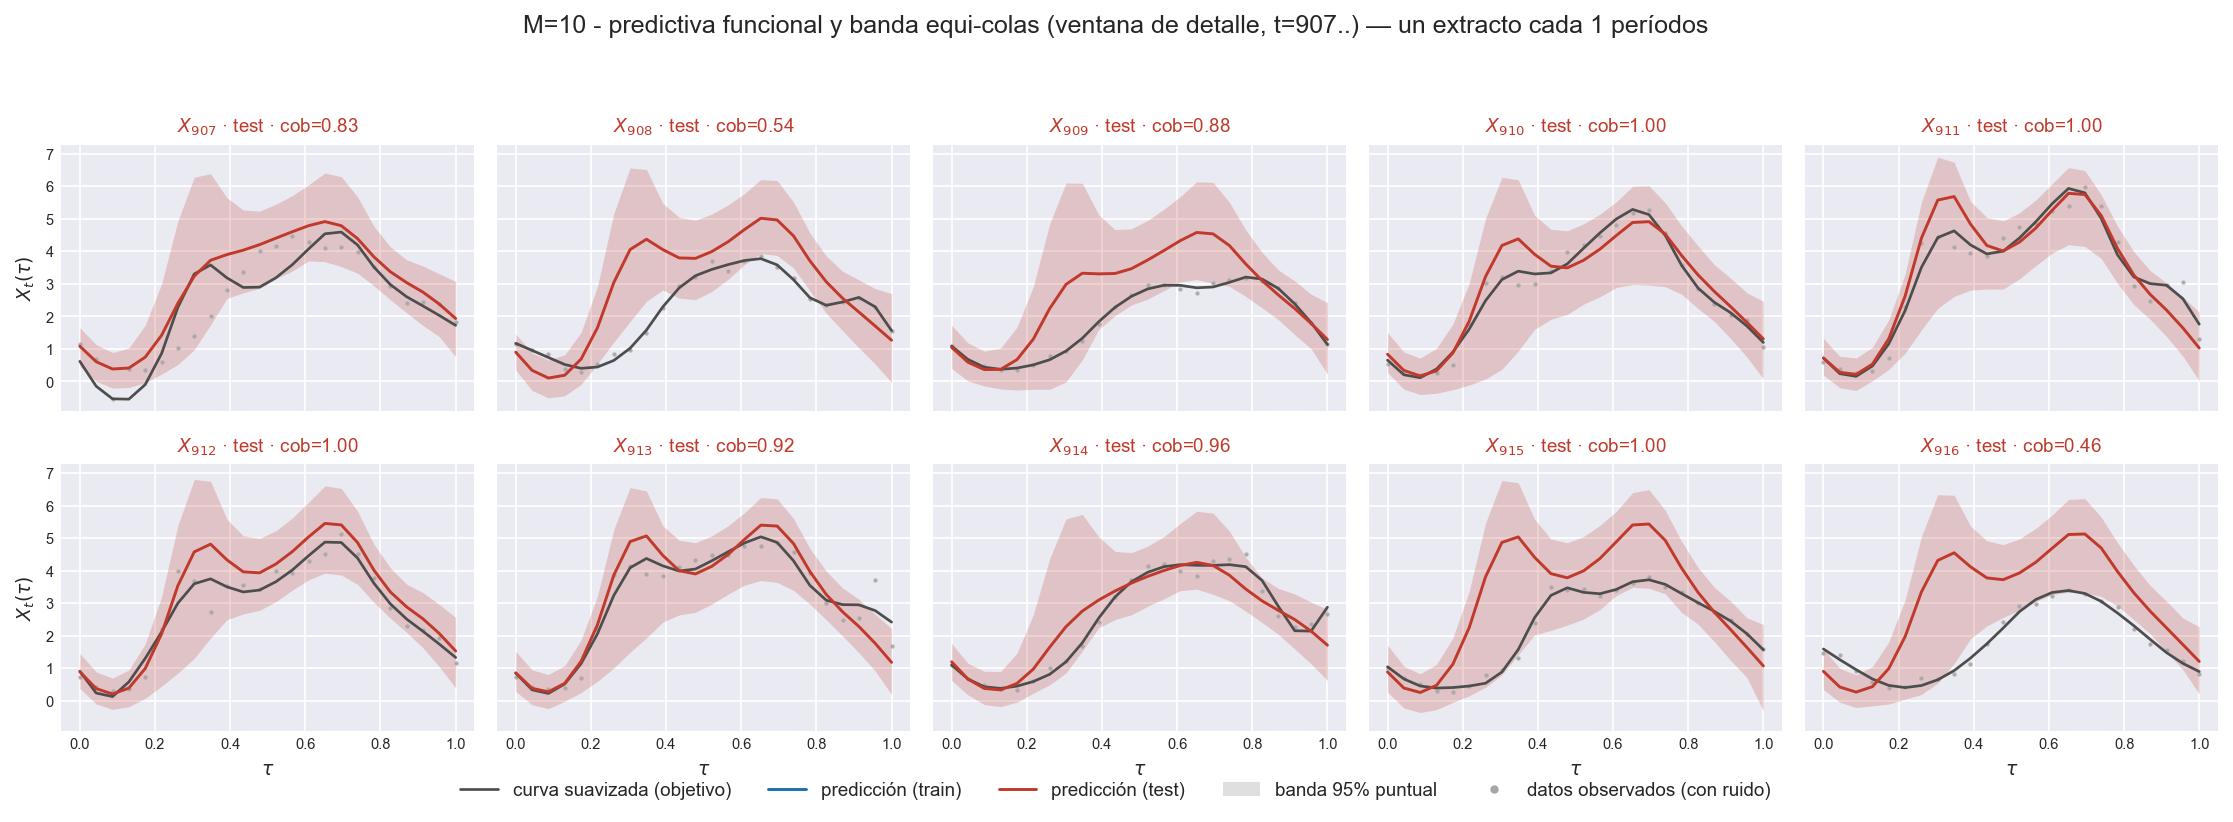
\includegraphics[width=\textwidth,height=0.8\textheight,keepaspectratio]{IMG/aneC_00/aneC_00_54_extractos_curvas_test_101.png}
\caption{Extractos de predicciones del bloque de prueba, tráfico $\{1\}$ ($M = 10$).}
\label{fig:aneC_54_extractos_curvas_test_101}
\end{figure}

\begin{figure}[H]
\centering
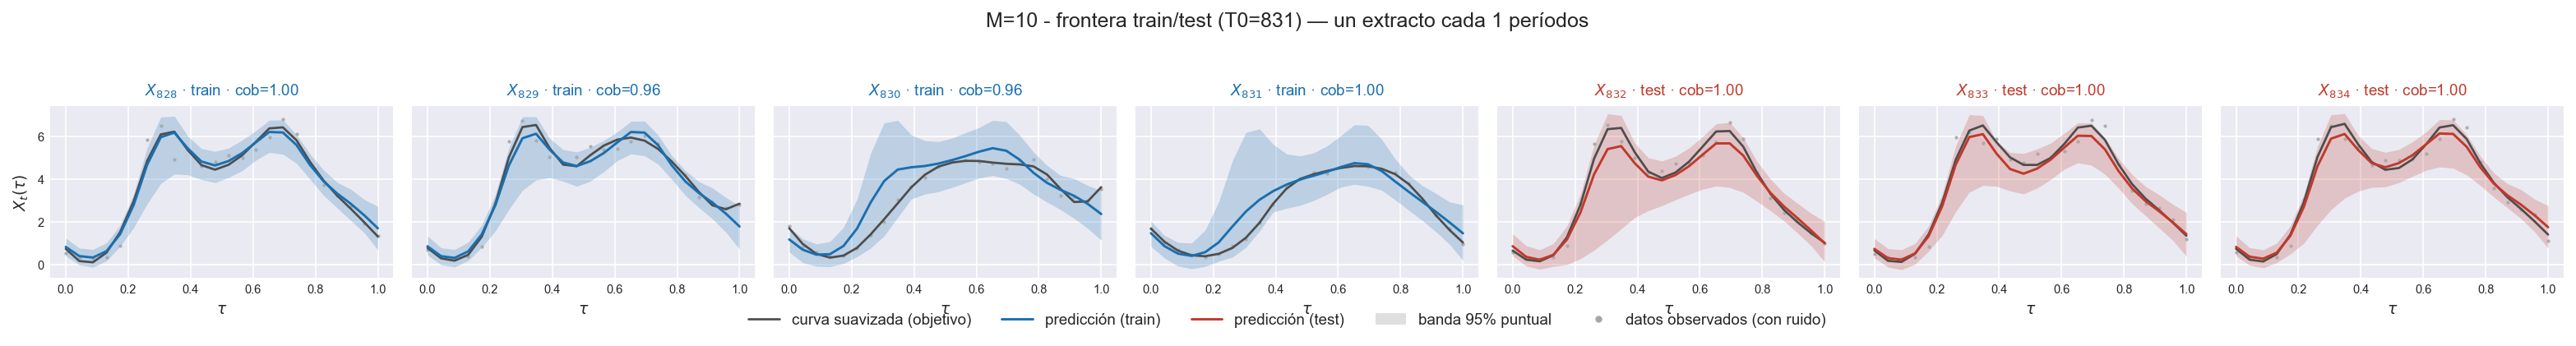
\includegraphics[width=\textwidth,height=0.8\textheight,keepaspectratio]{IMG/aneC_00/aneC_00_55_extractos_frontera_101.png}
\caption{Predicciones en la frontera entre train y test, tráfico $\{1\}$ ($M = 10$).}
\label{fig:aneC_55_extractos_frontera_101}
\end{figure}

\begin{figure}[H]
\centering
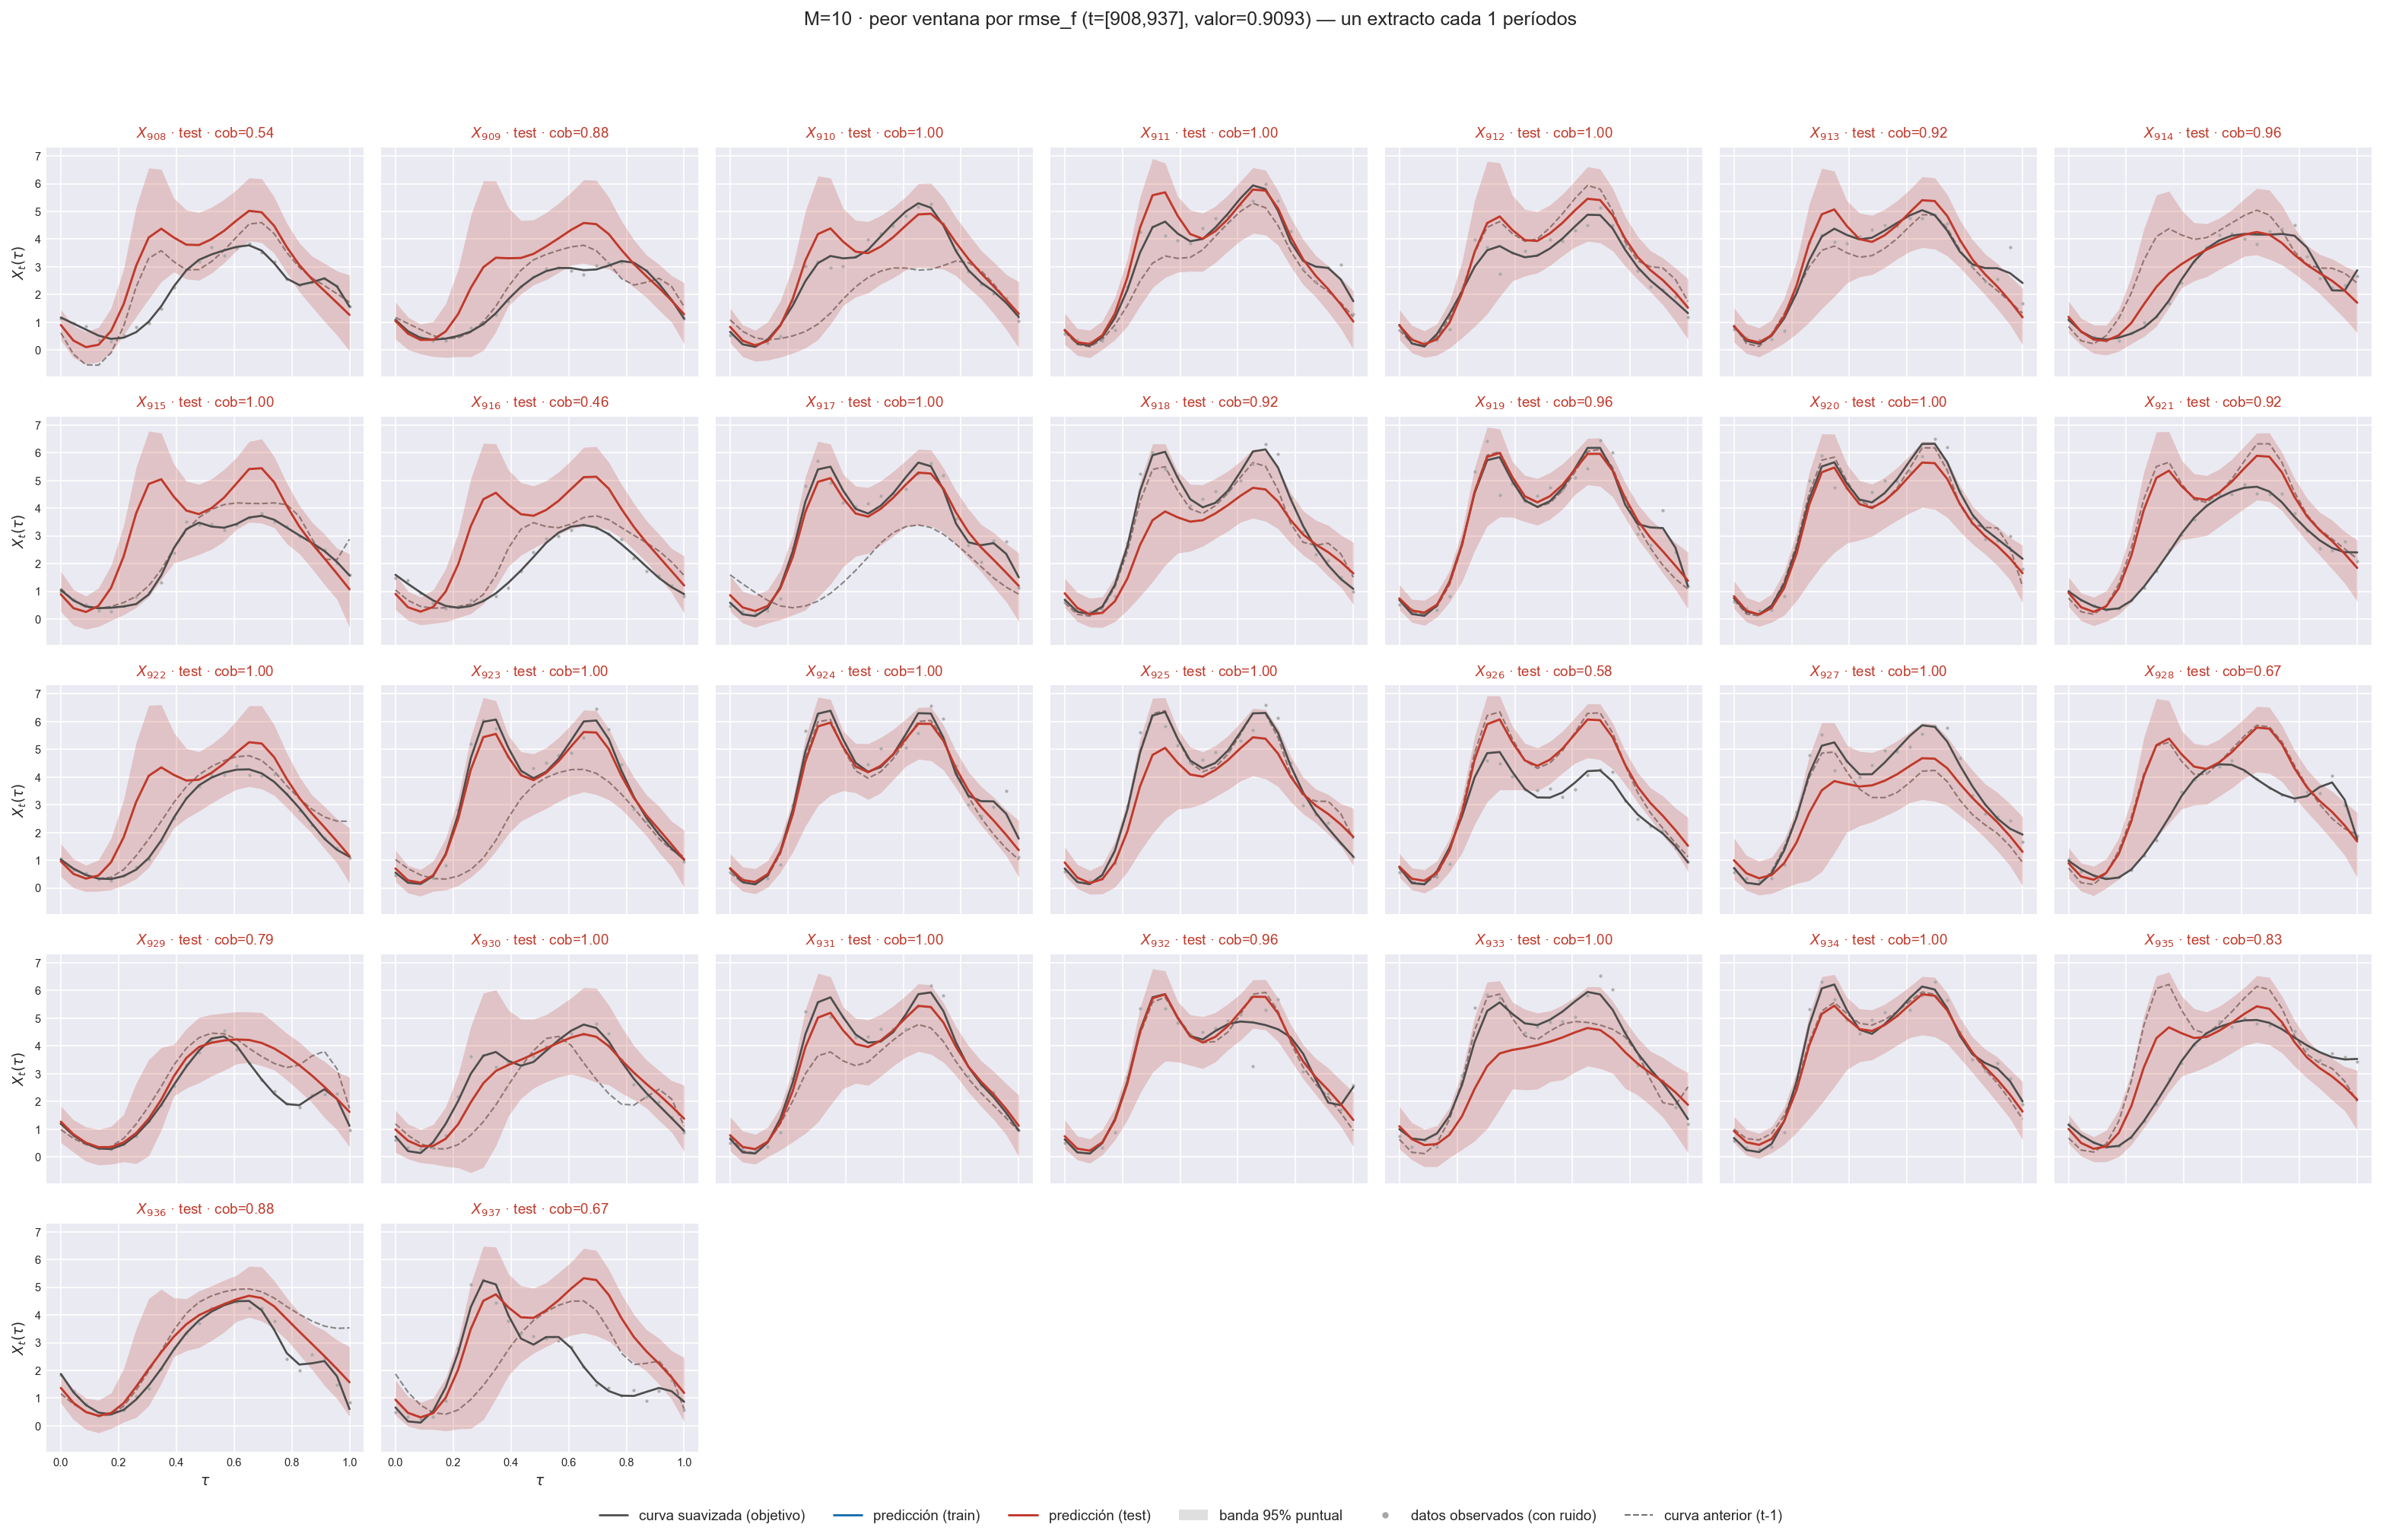
\includegraphics[width=\textwidth,height=0.8\textheight,keepaspectratio]{IMG/aneC_00/aneC_00_56b_peor_ventana_rmse_f_t908_101.png}
\caption{Ventana de peor RMSE (origen $t = 908$), tráfico $\{1\}$ ($M = 10$).}
\label{fig:aneC_56b_peor_ventana_rmse_f_t908_101}
\end{figure}

\begin{figure}[H]
\centering
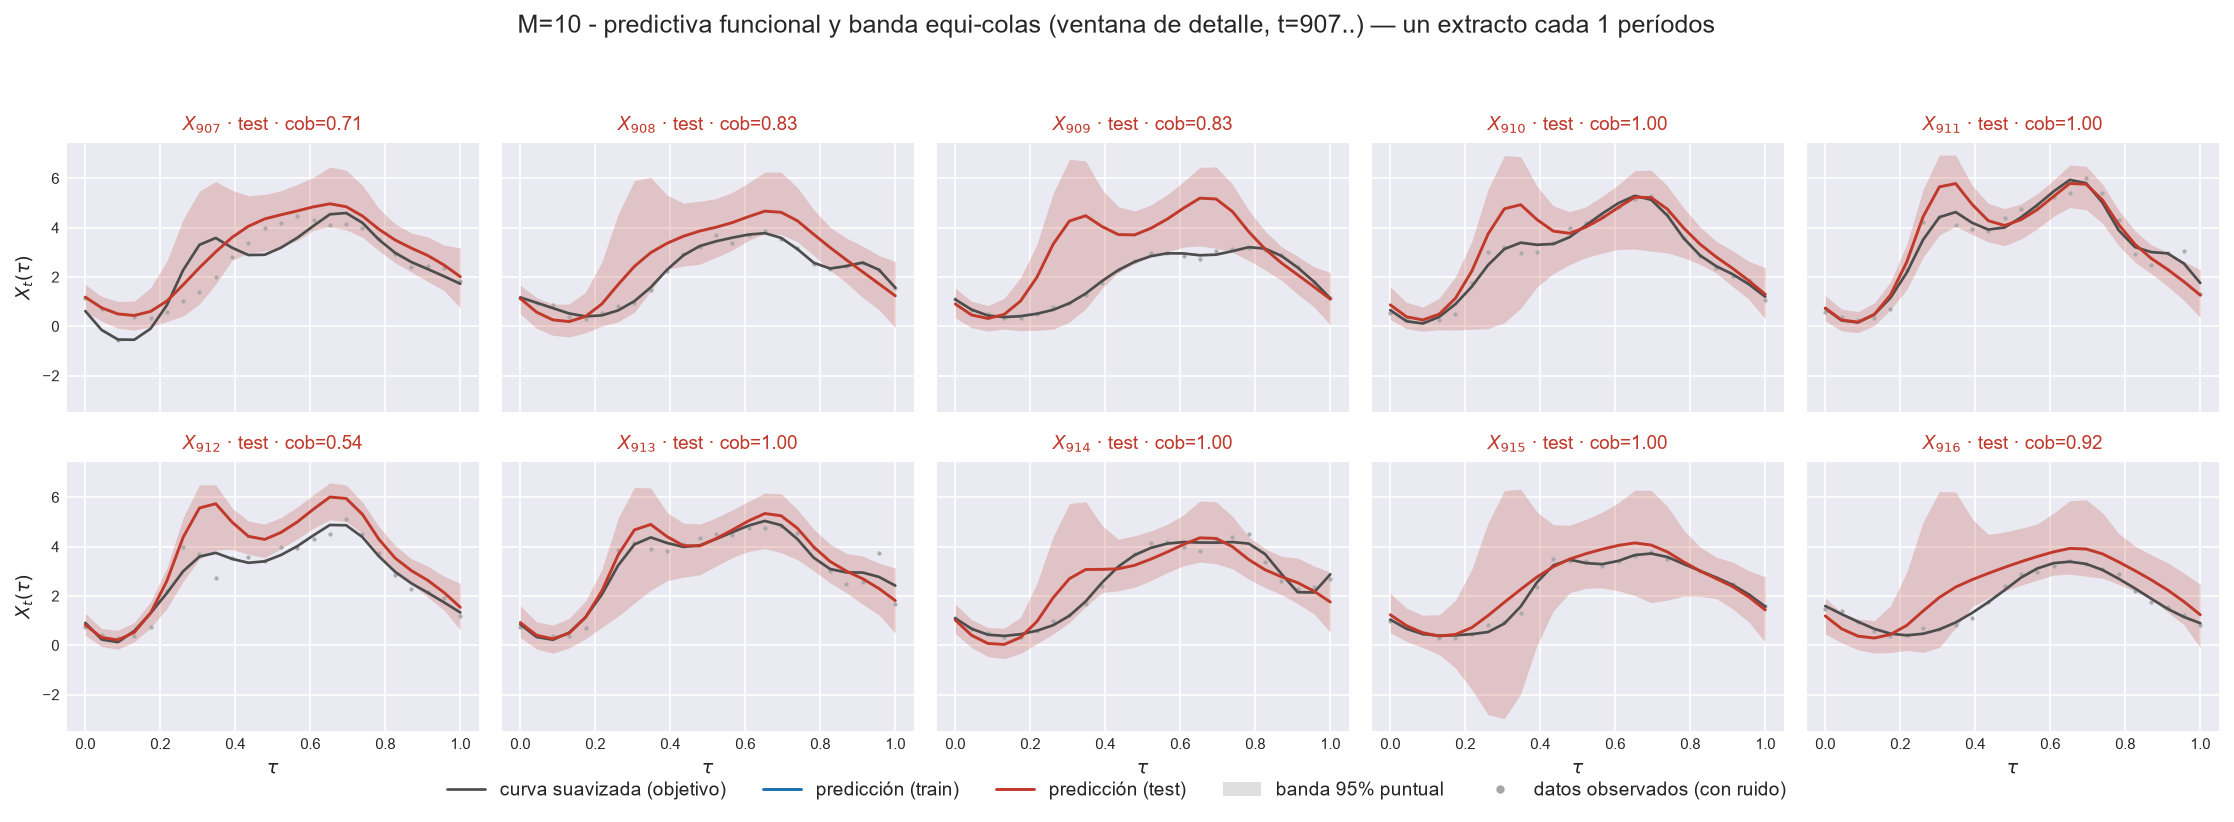
\includegraphics[width=\textwidth,height=0.8\textheight,keepaspectratio]{IMG/aneC_00/aneC_00_54_extractos_curvas_test_102.png}
\caption{Extractos de predicciones del bloque de prueba, tráfico $\{1,7\}$ ($M = 10$).}
\label{fig:aneC_54_extractos_curvas_test_102}
\end{figure}

\begin{figure}[H]
\centering
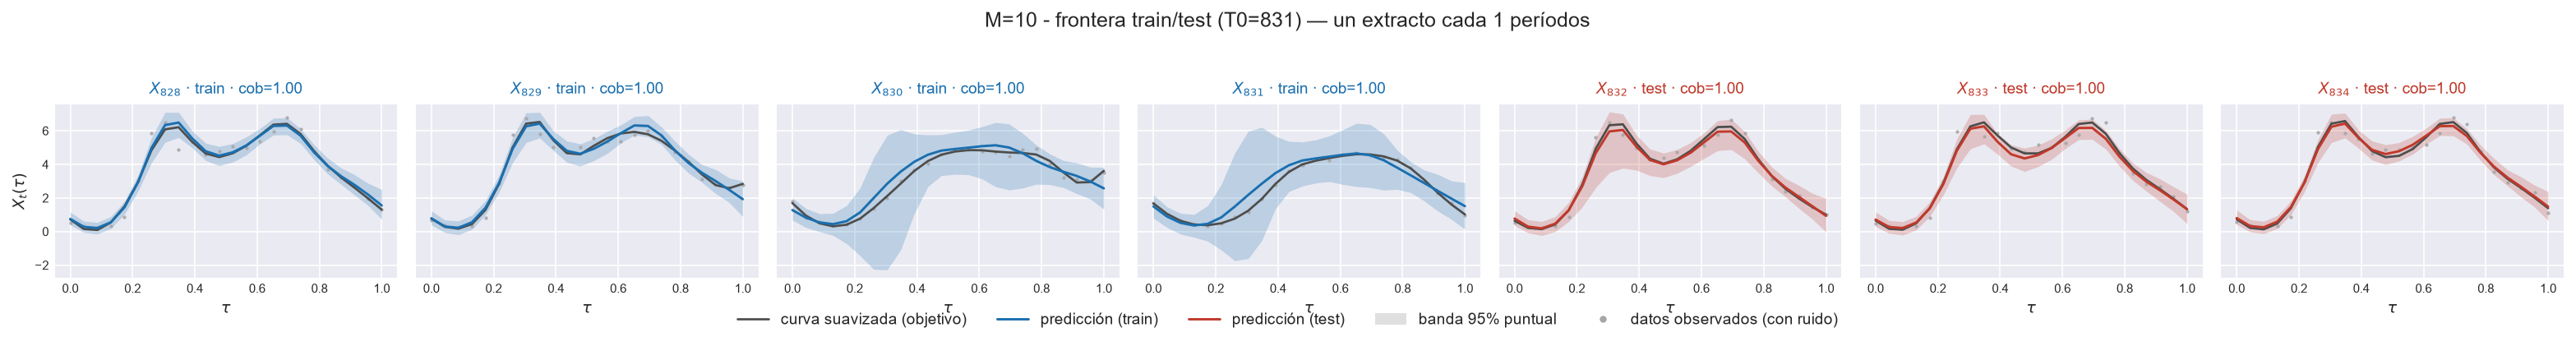
\includegraphics[width=\textwidth,height=0.8\textheight,keepaspectratio]{IMG/aneC_00/aneC_00_55_extractos_frontera_102.png}
\caption{Predicciones en la frontera entre train y test, tráfico $\{1,7\}$ ($M = 10$).}
\label{fig:aneC_55_extractos_frontera_102}
\end{figure}

\begin{figure}[H]
\centering
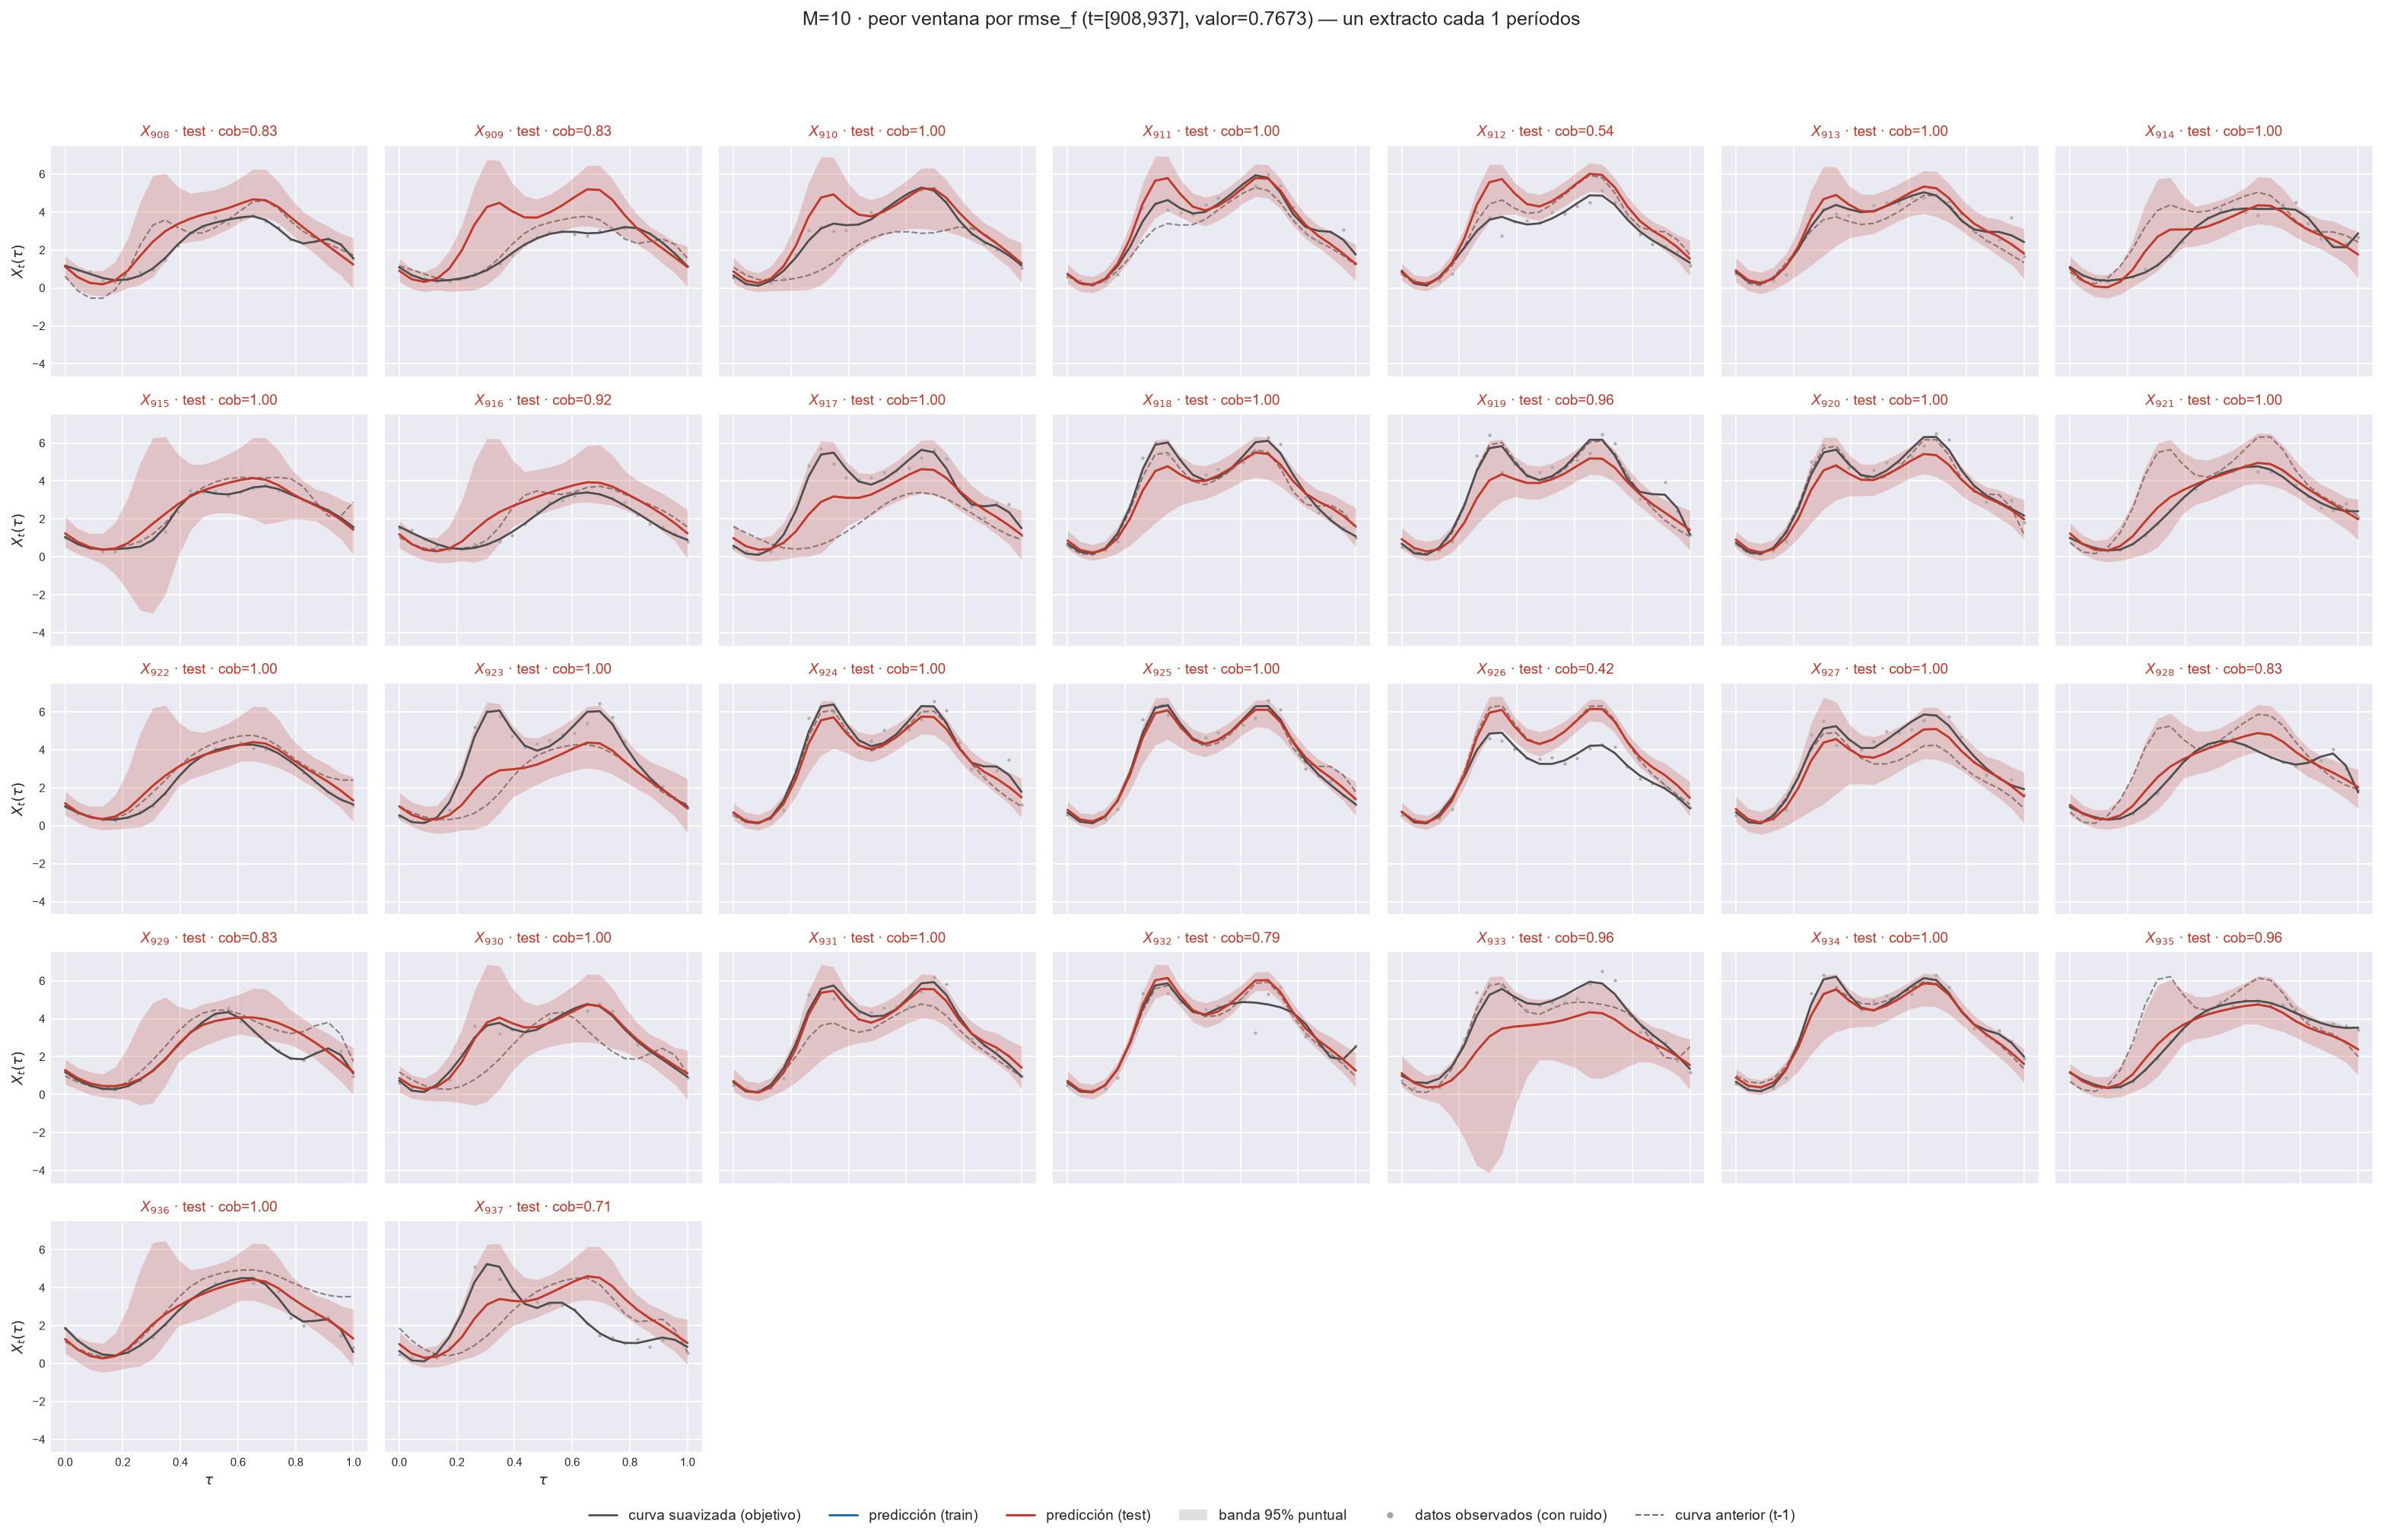
\includegraphics[width=\textwidth,height=0.8\textheight,keepaspectratio]{IMG/aneC_00/aneC_00_56b_peor_ventana_rmse_f_t908_102.png}
\caption{Ventana de peor RMSE (origen $t = 908$), tráfico $\{1,7\}$ ($M = 10$).}
\label{fig:aneC_56b_peor_ventana_rmse_f_t908_102}
\end{figure}

\section{Comportamientos predictivos}
\label{aneC_00_04_comportamientos}
% 61: predictores y draws; 63: ventana de detalle t = 907..916 de a dos; 64: catálogo global; 102b: K a lo largo de la serie.

\begin{figure}[H]
\centering
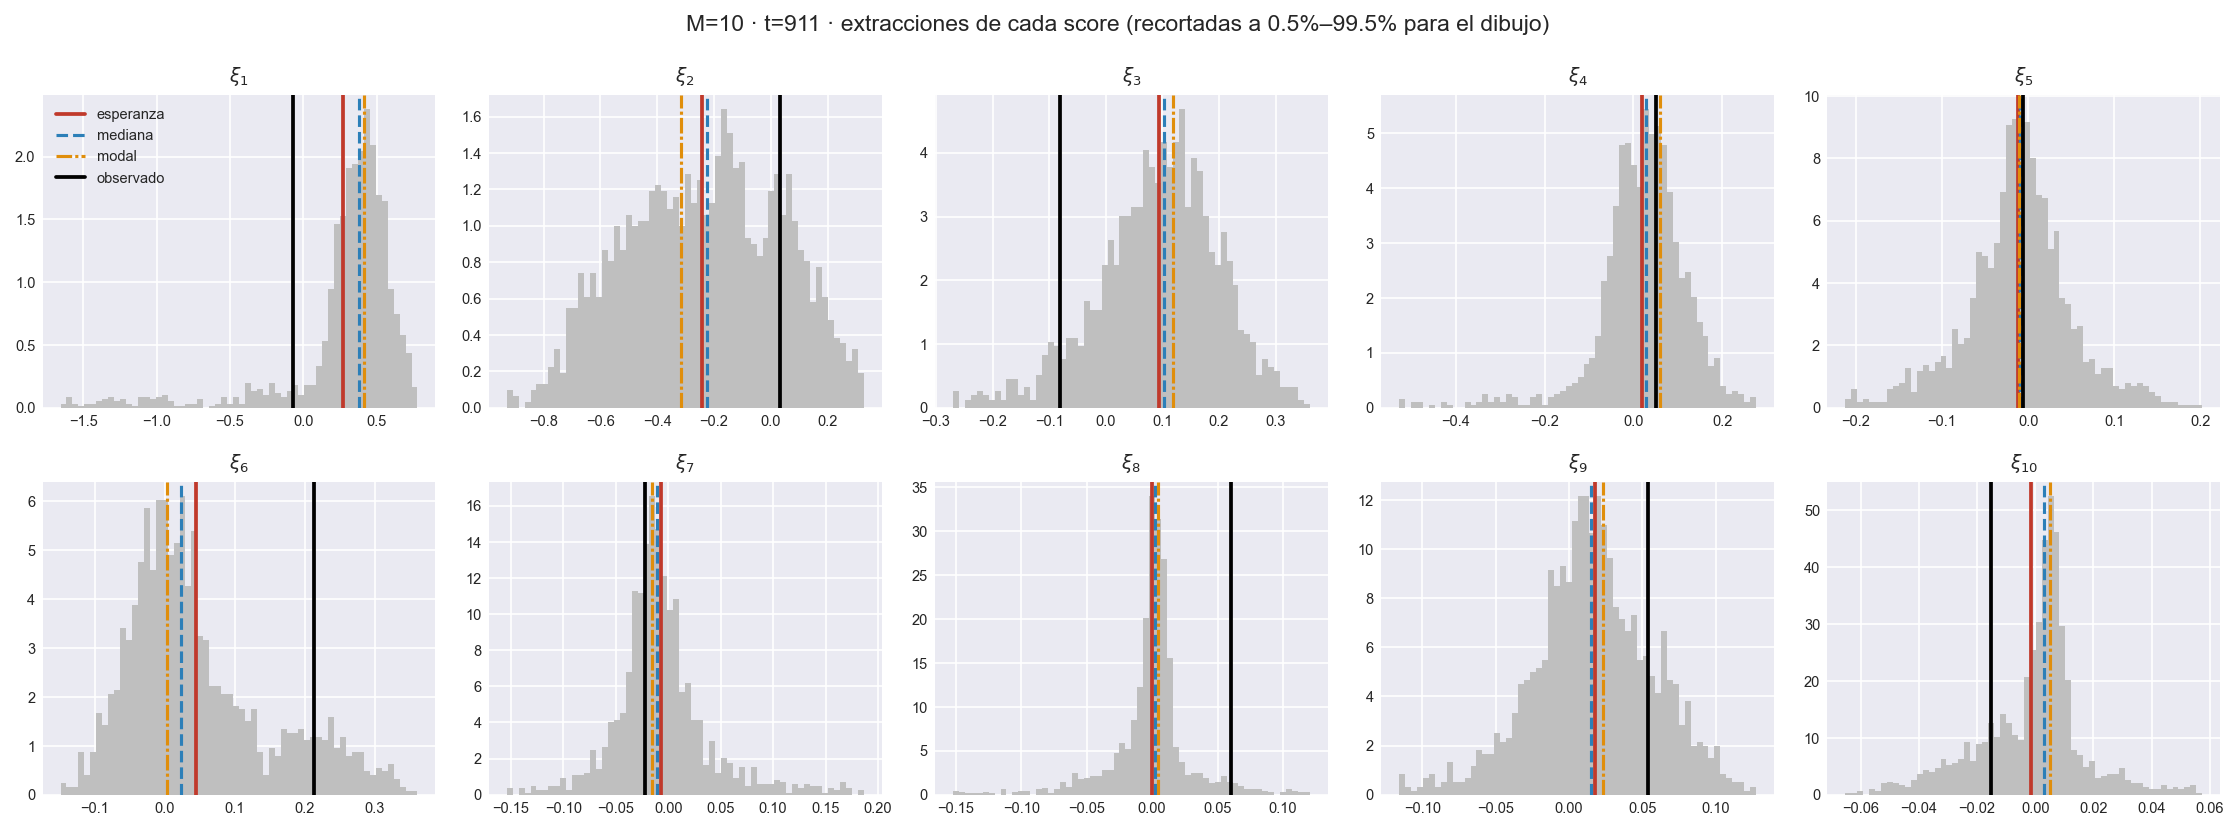
\includegraphics[width=\textwidth,height=0.6\textheight,keepaspectratio]{IMG/aneC_00/aneC_00_61_histogramas_draws_101.png}
\caption{Histograma de las extracciones del score en un origen con más de un comportamiento, tráfico $\{1\}$ ($M = 10$).}
\label{fig:aneC_hist_101}
\end{figure}

\begin{figure}[H]
\centering
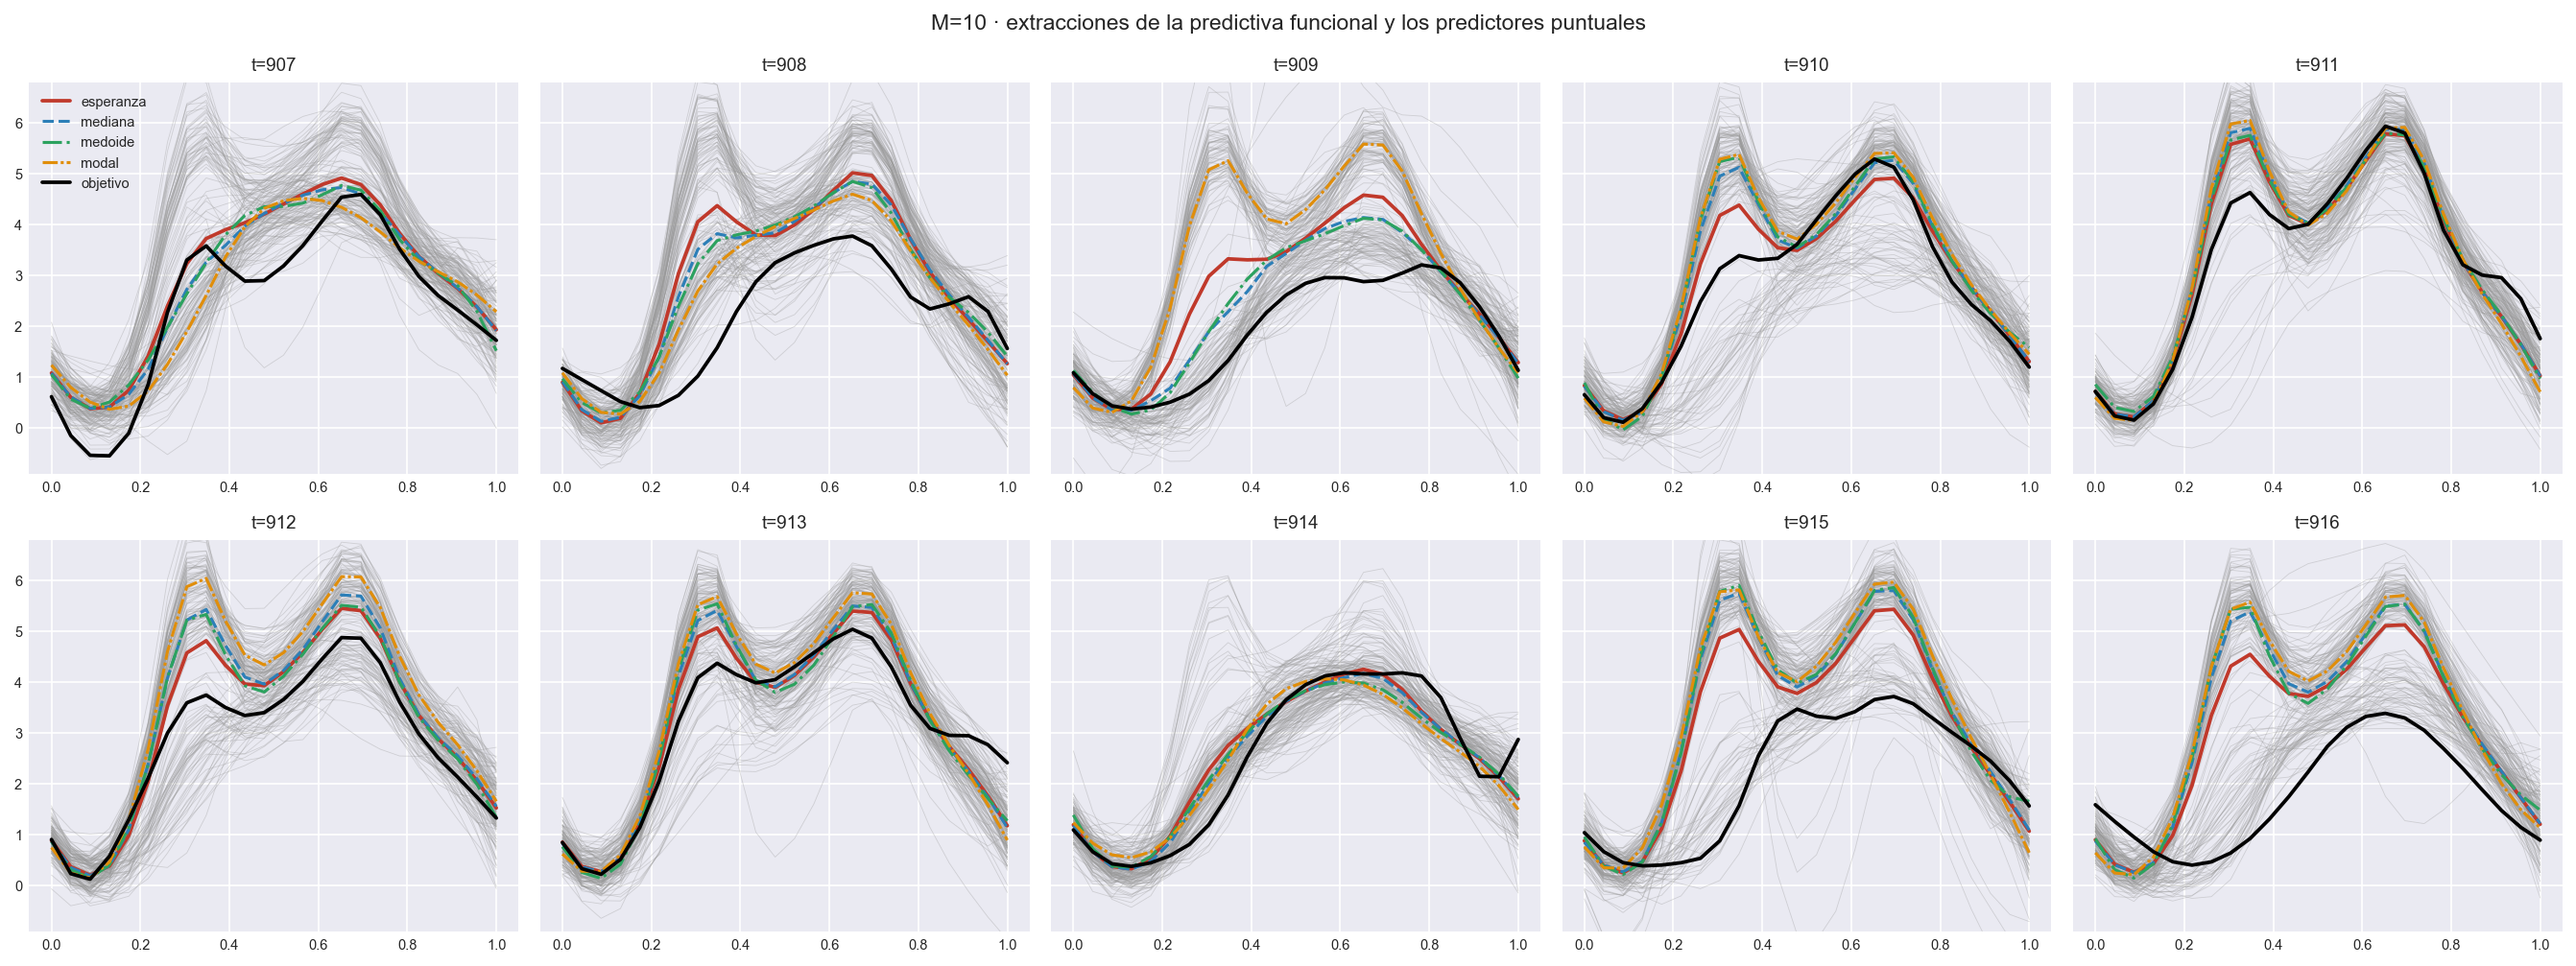
\includegraphics[width=\textwidth,height=0.8\textheight,keepaspectratio]{IMG/aneC_00/aneC_00_61b_curvas_predictores_101.png}
\caption{Curvas de los predictores puntuales en orígenes con más de un comportamiento, tráfico $\{1\}$ ($M = 10$).}
\label{fig:aneC_predictores_101}
\end{figure}

\begin{figure}[H]
\centering
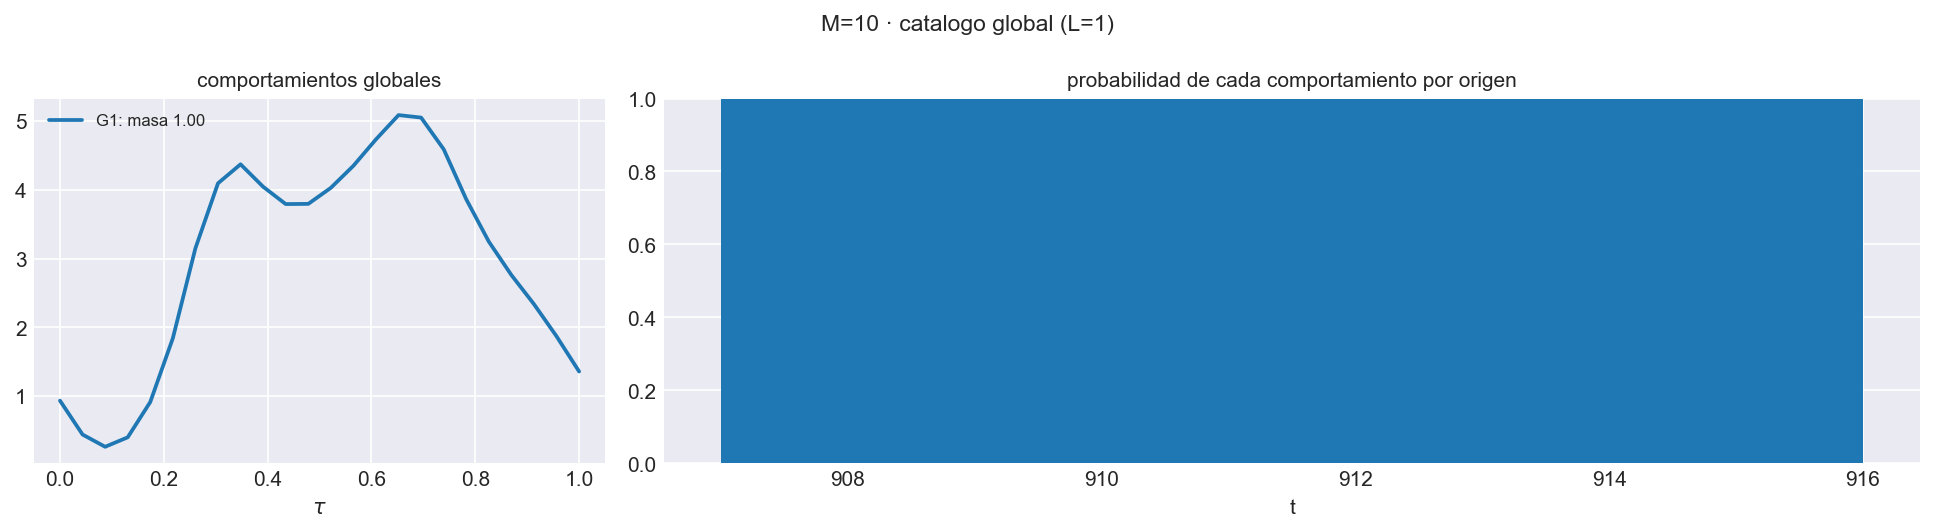
\includegraphics[width=\textwidth,height=0.6\textheight,keepaspectratio]{IMG/aneC_00/aneC_00_64_catalogo_global_101.png}
\caption{Catálogo global de comportamientos, tráfico $\{1\}$ ($M = 10$).}
\label{fig:aneC_catalogo_101}
\end{figure}

\begin{figure}[H]
\centering
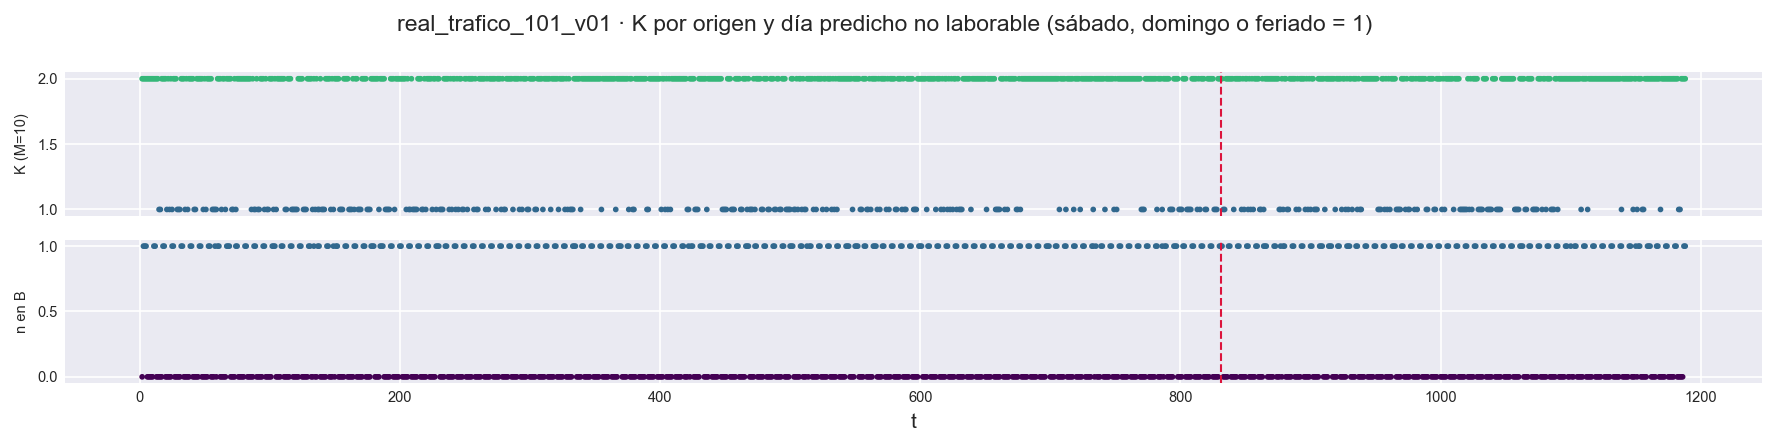
\includegraphics[width=\textwidth,height=0.6\textheight,keepaspectratio]{IMG/aneC_00/aneC_00_102b_K_serie_101.png}
\caption{Número de comportamientos $K_t$ a lo largo de la serie, tráfico $\{1\}$ ($M = 10$).}
\label{fig:aneC_Kserie_101}
\end{figure}

\begin{figure}[H]
\centering
\begin{minipage}{0.49\textwidth}\centering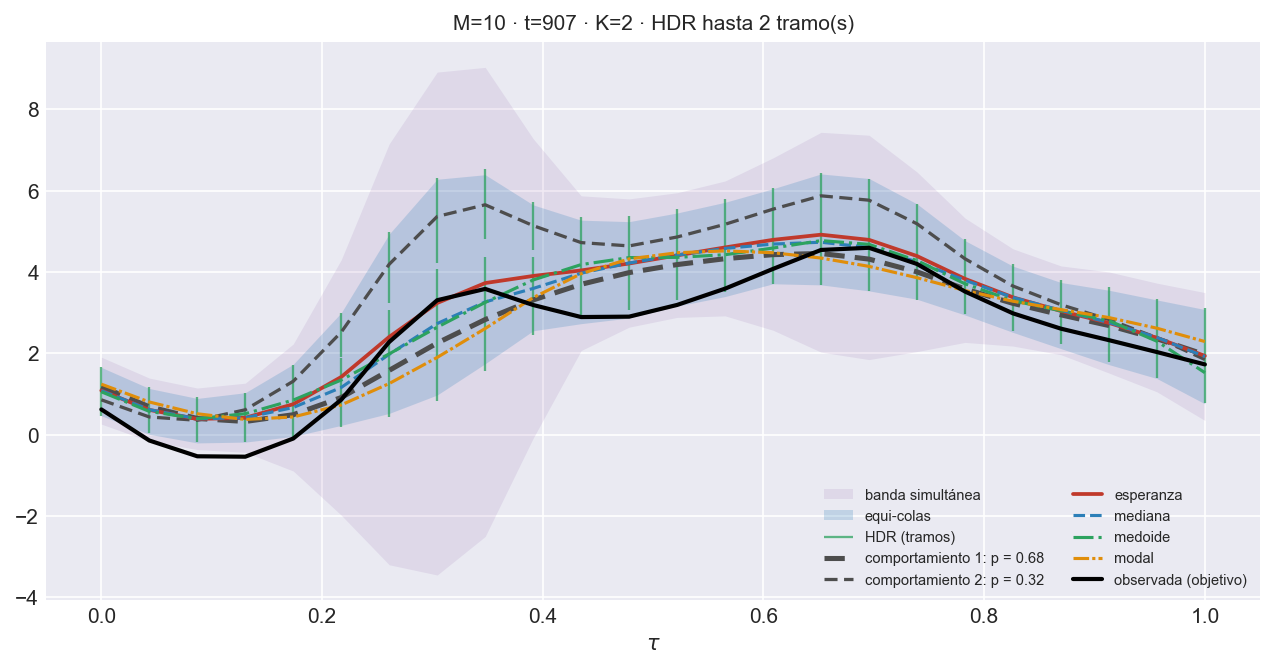
\includegraphics[width=\textwidth,height=0.4\textheight,keepaspectratio]{IMG/aneC_00/aneC_00_63_detalle_t907_101.png}\end{minipage}\hfill
\begin{minipage}{0.49\textwidth}\centering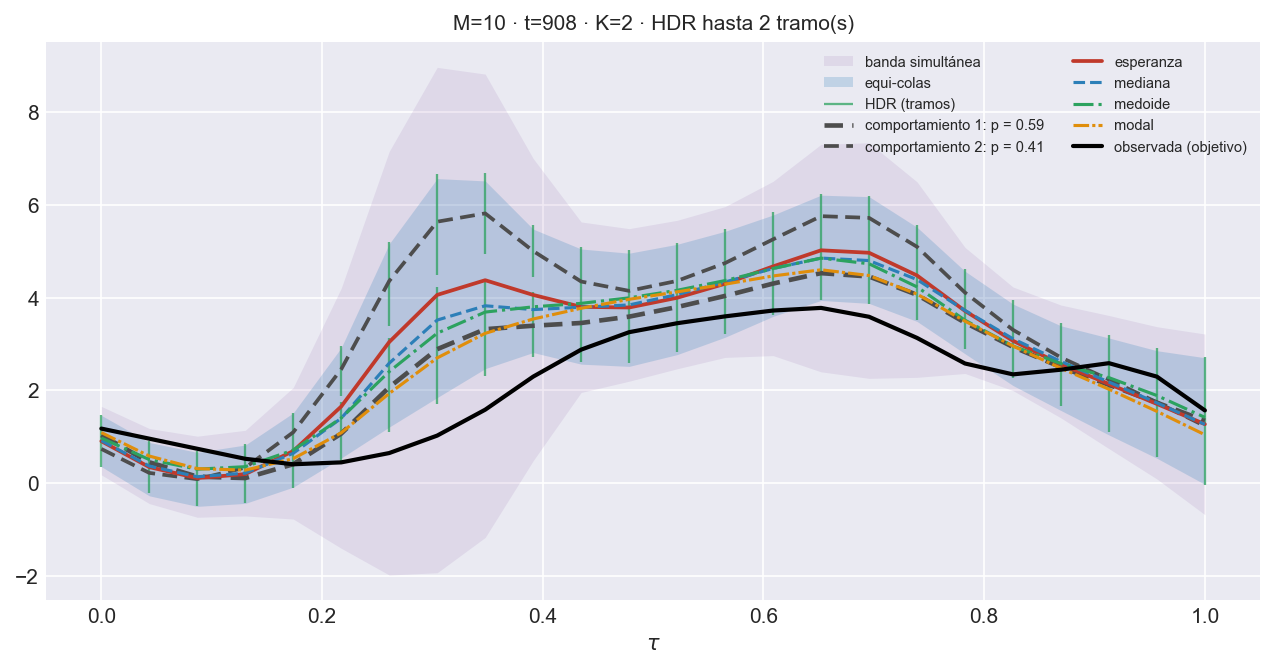
\includegraphics[width=\textwidth,height=0.4\textheight,keepaspectratio]{IMG/aneC_00/aneC_00_63_detalle_t908_101.png}\end{minipage}
\caption{Ventana de detalle, tráfico $\{1\}$, orígenes $t = 907$ y $t = 908$ ($M = 10$).}
\label{fig:aneC_detalle_907_101}
\end{figure}

\begin{figure}[H]
\centering
\begin{minipage}{0.49\textwidth}\centering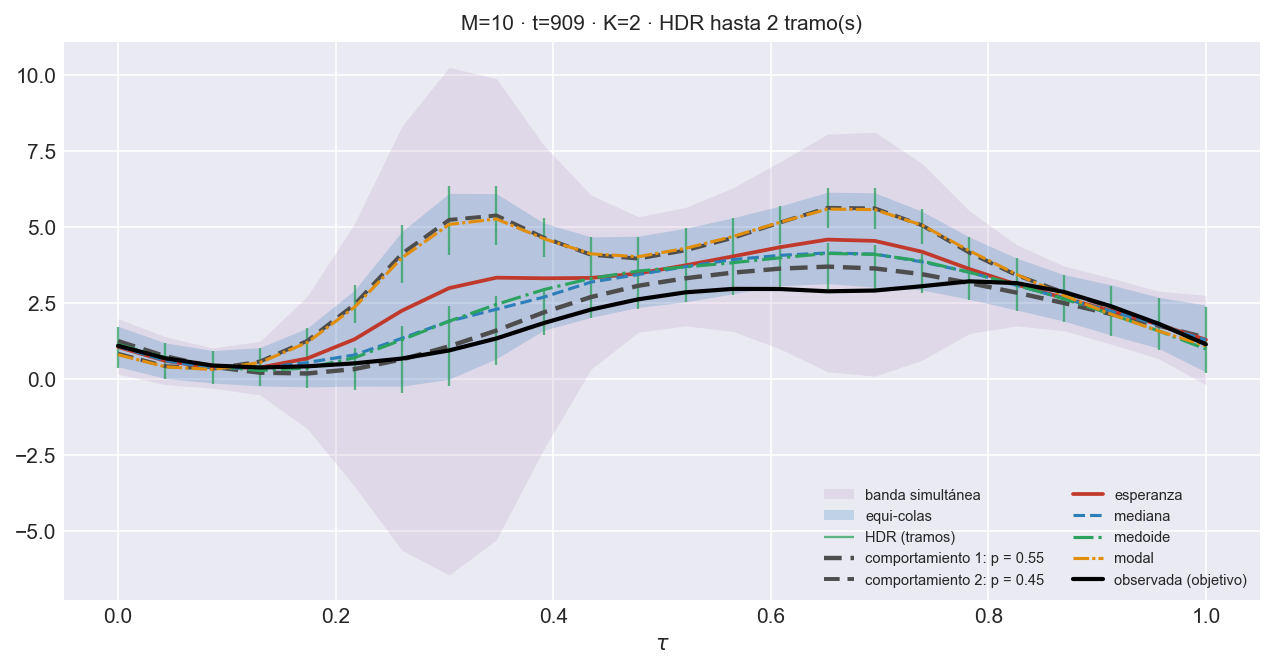
\includegraphics[width=\textwidth,height=0.4\textheight,keepaspectratio]{IMG/aneC_00/aneC_00_63_detalle_t909_101.png}\end{minipage}\hfill
\begin{minipage}{0.49\textwidth}\centering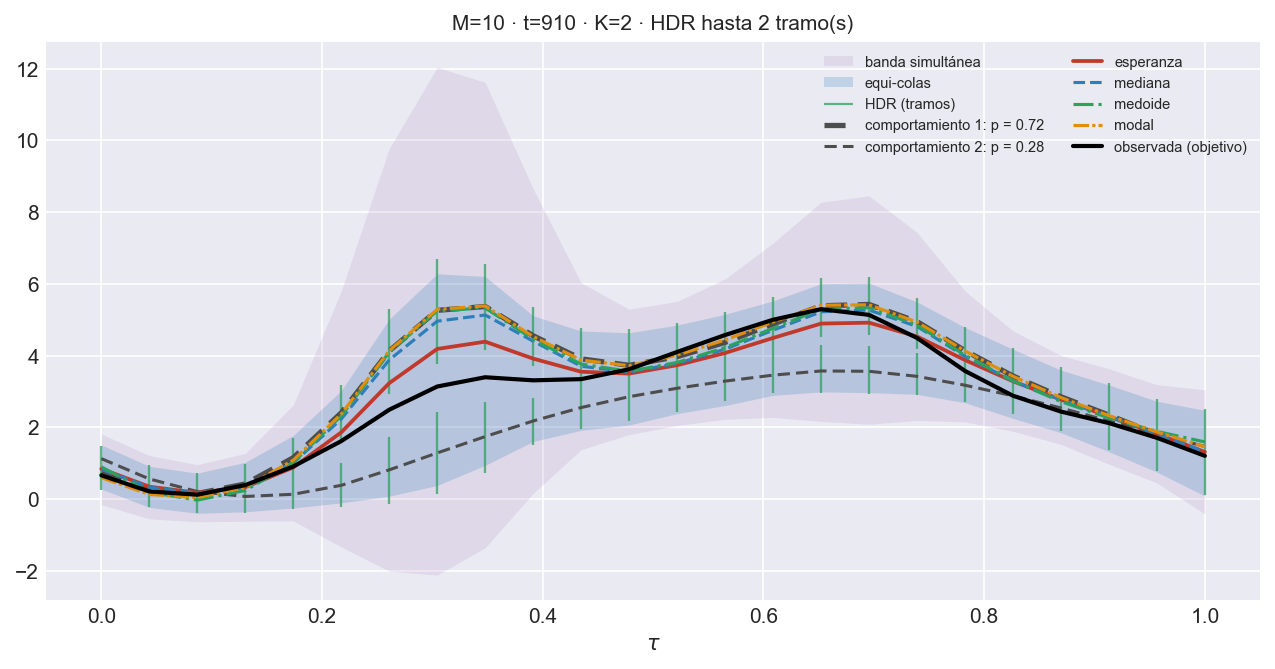
\includegraphics[width=\textwidth,height=0.4\textheight,keepaspectratio]{IMG/aneC_00/aneC_00_63_detalle_t910_101.png}\end{minipage}
\caption{Ventana de detalle, tráfico $\{1\}$, orígenes $t = 909$ y $t = 910$ ($M = 10$).}
\label{fig:aneC_detalle_909_101}
\end{figure}

\begin{figure}[H]
\centering
\begin{minipage}{0.49\textwidth}\centering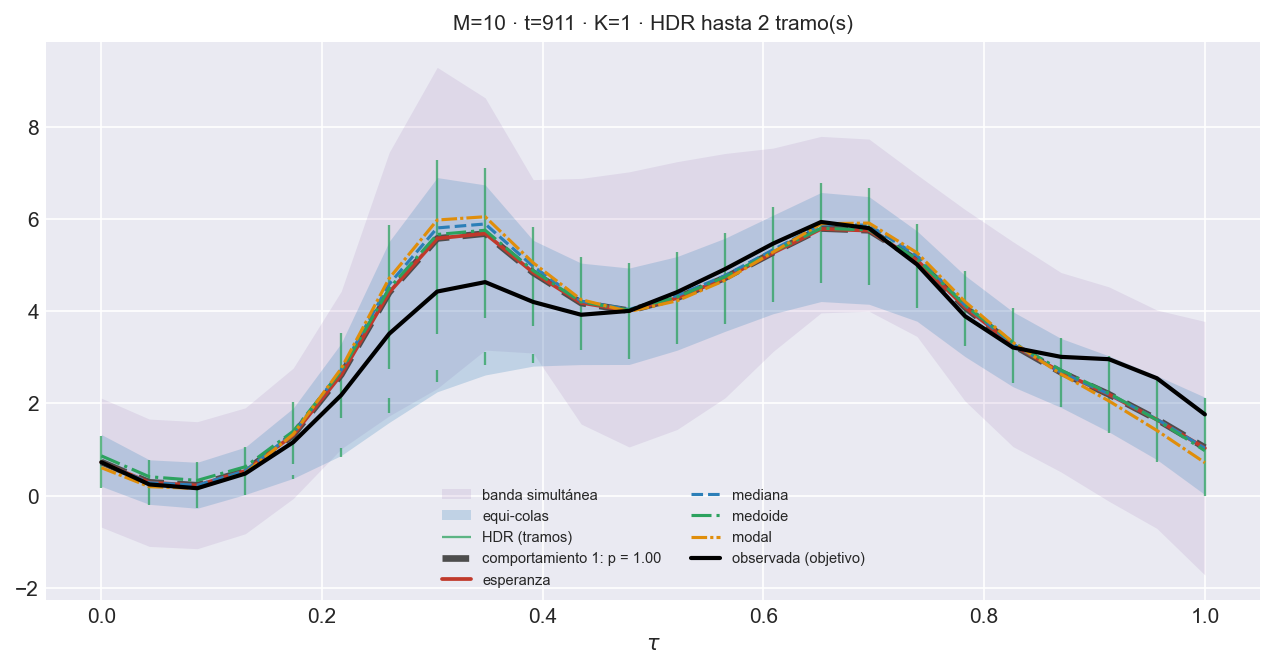
\includegraphics[width=\textwidth,height=0.4\textheight,keepaspectratio]{IMG/aneC_00/aneC_00_63_detalle_t911_101.png}\end{minipage}\hfill
\begin{minipage}{0.49\textwidth}\centering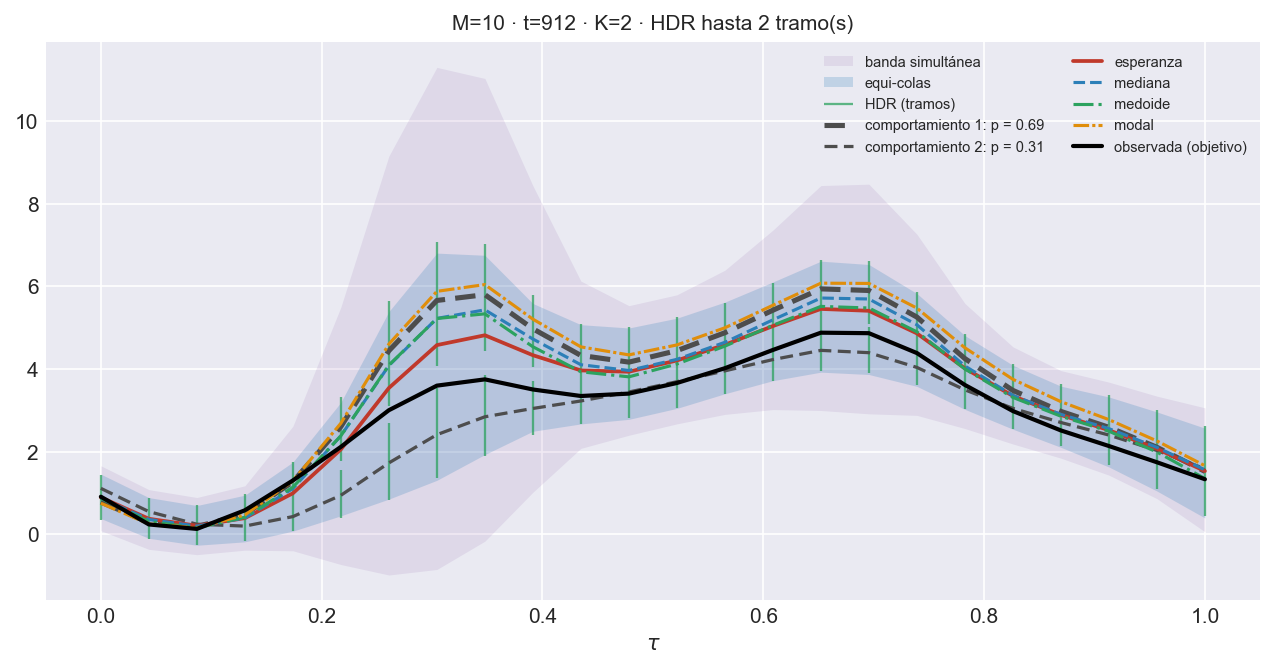
\includegraphics[width=\textwidth,height=0.4\textheight,keepaspectratio]{IMG/aneC_00/aneC_00_63_detalle_t912_101.png}\end{minipage}
\caption{Ventana de detalle, tráfico $\{1\}$, orígenes $t = 911$ y $t = 912$ ($M = 10$).}
\label{fig:aneC_detalle_911_101}
\end{figure}

\begin{figure}[H]
\centering
\begin{minipage}{0.49\textwidth}\centering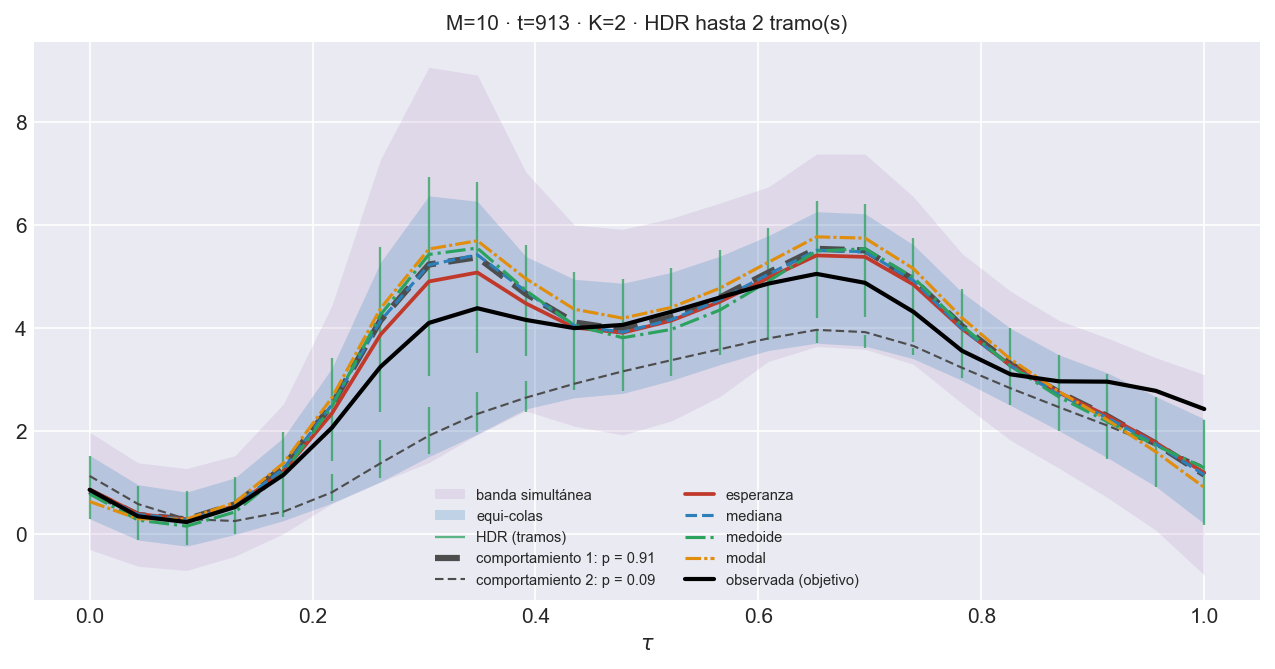
\includegraphics[width=\textwidth,height=0.4\textheight,keepaspectratio]{IMG/aneC_00/aneC_00_63_detalle_t913_101.png}\end{minipage}\hfill
\begin{minipage}{0.49\textwidth}\centering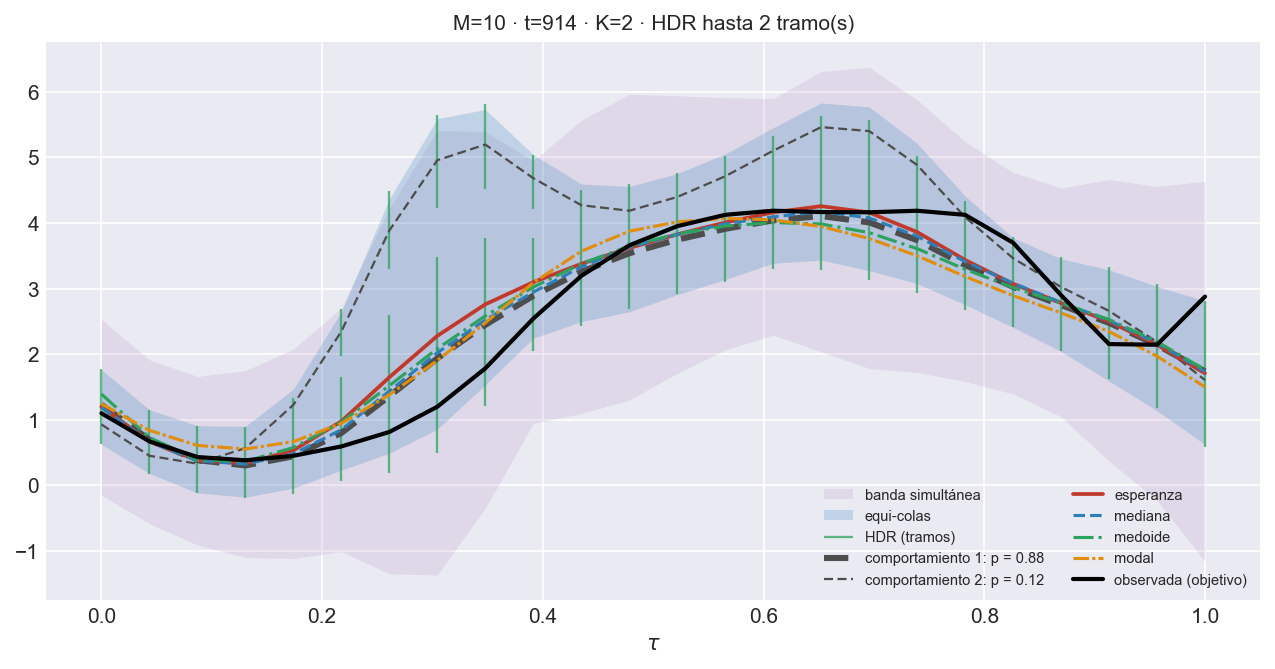
\includegraphics[width=\textwidth,height=0.4\textheight,keepaspectratio]{IMG/aneC_00/aneC_00_63_detalle_t914_101.png}\end{minipage}
\caption{Ventana de detalle, tráfico $\{1\}$, orígenes $t = 913$ y $t = 914$ ($M = 10$).}
\label{fig:aneC_detalle_913_101}
\end{figure}

\begin{figure}[H]
\centering
\begin{minipage}{0.49\textwidth}\centering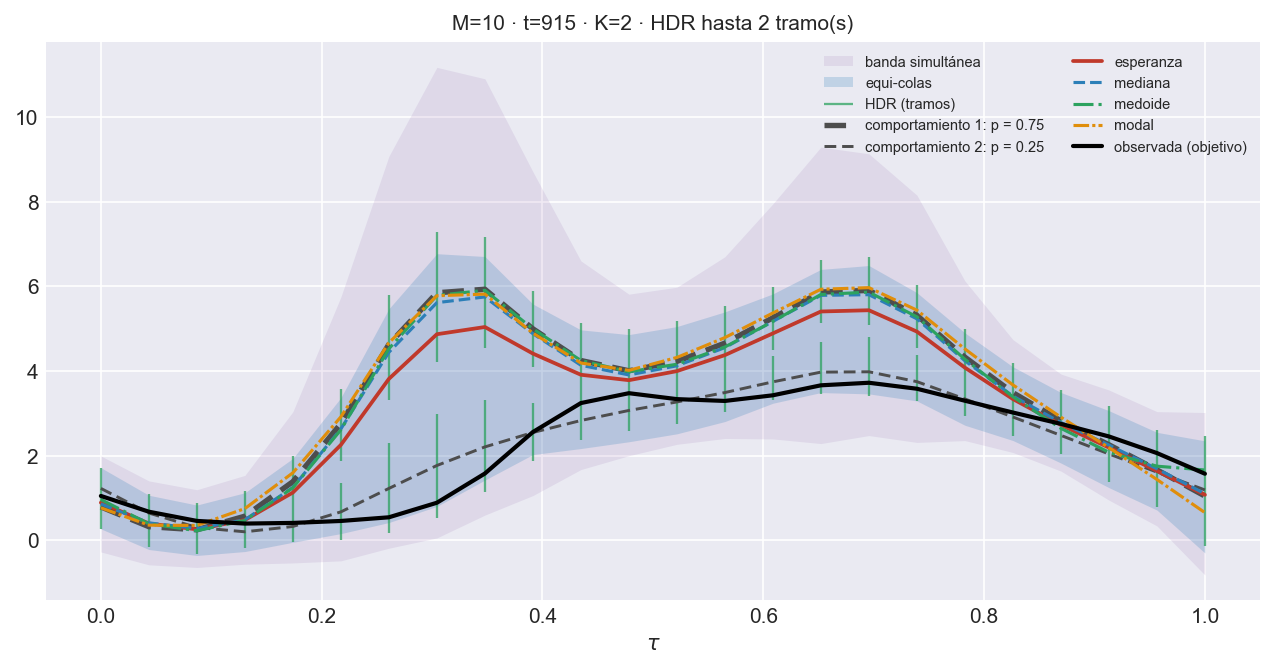
\includegraphics[width=\textwidth,height=0.4\textheight,keepaspectratio]{IMG/aneC_00/aneC_00_63_detalle_t915_101.png}\end{minipage}\hfill
\begin{minipage}{0.49\textwidth}\centering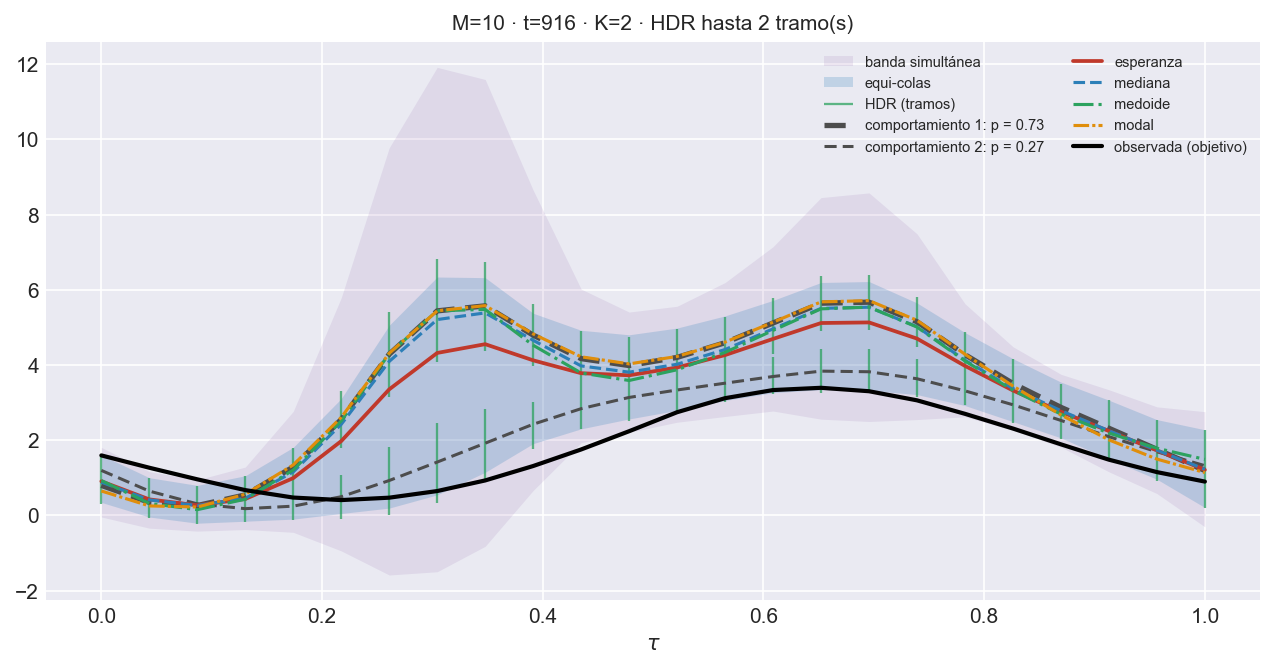
\includegraphics[width=\textwidth,height=0.4\textheight,keepaspectratio]{IMG/aneC_00/aneC_00_63_detalle_t916_101.png}\end{minipage}
\caption{Ventana de detalle, tráfico $\{1\}$, orígenes $t = 915$ y $t = 916$ ($M = 10$).}
\label{fig:aneC_detalle_915_101}
\end{figure}

\begin{figure}[H]
\centering
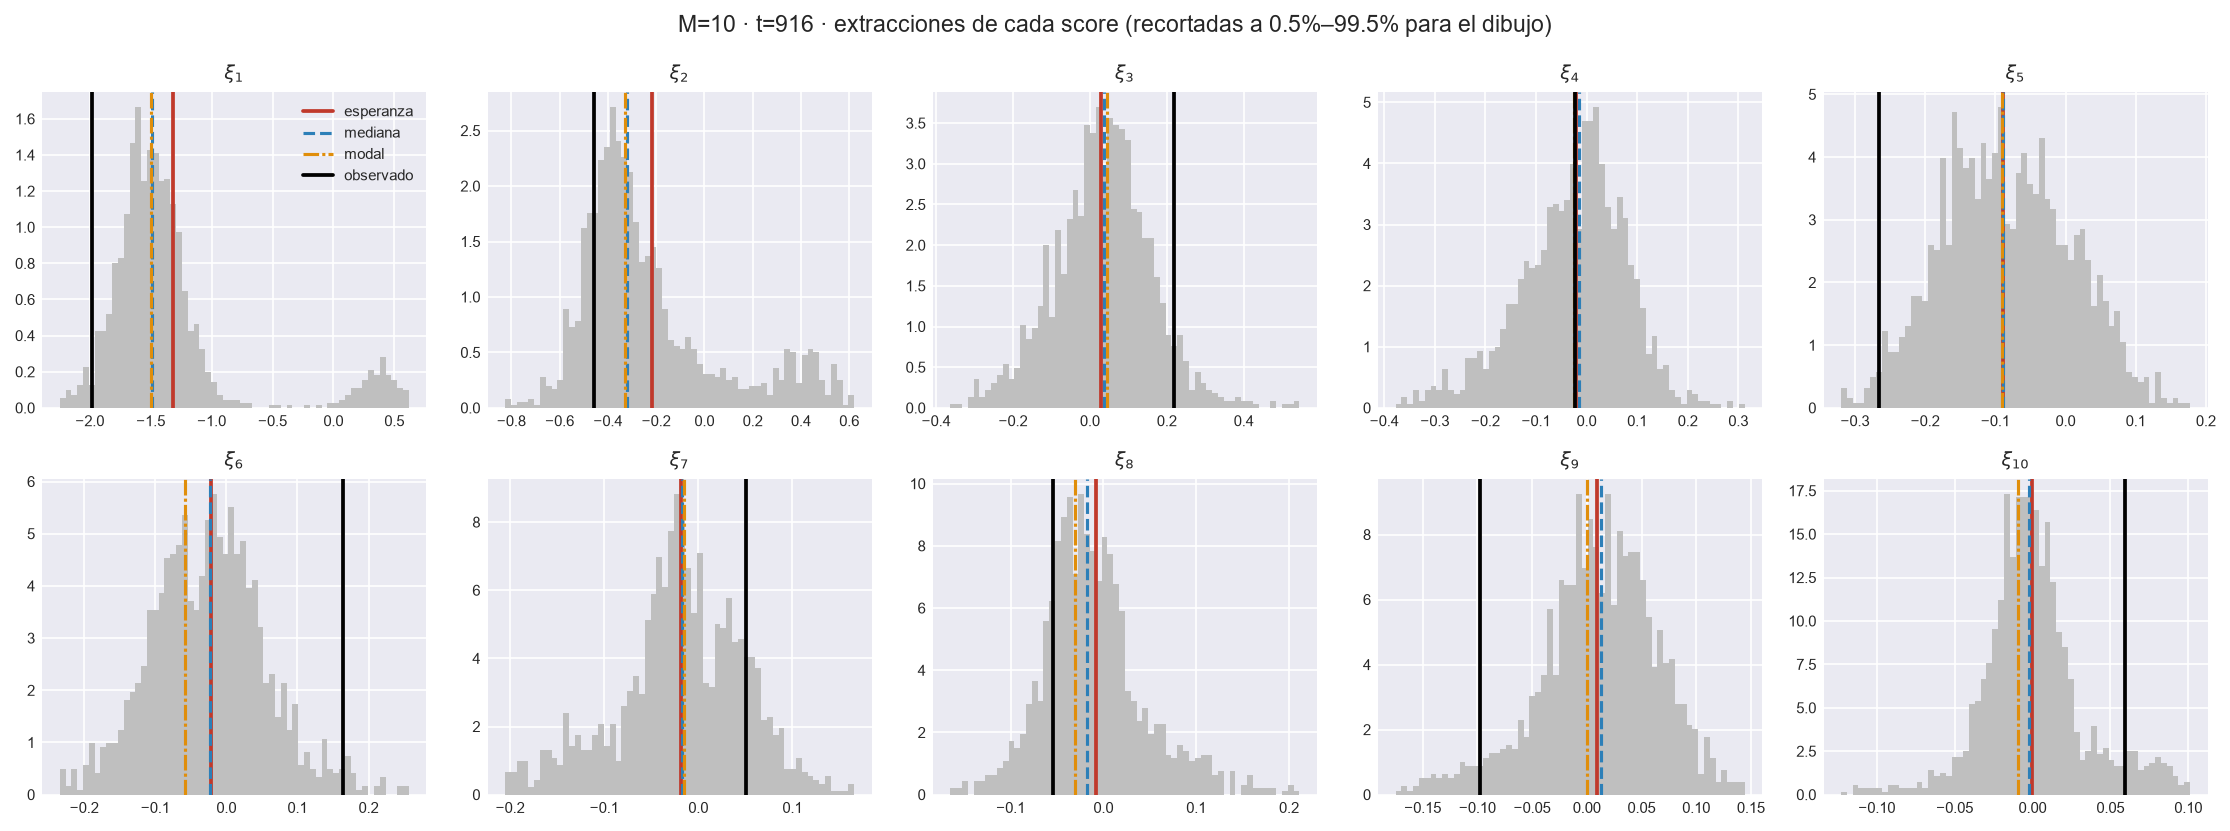
\includegraphics[width=\textwidth,height=0.6\textheight,keepaspectratio]{IMG/aneC_00/aneC_00_61_histogramas_draws_102.png}
\caption{Histograma de las extracciones del score en un origen con más de un comportamiento, tráfico $\{1,7\}$ ($M = 10$).}
\label{fig:aneC_hist_102}
\end{figure}

\begin{figure}[H]
\centering
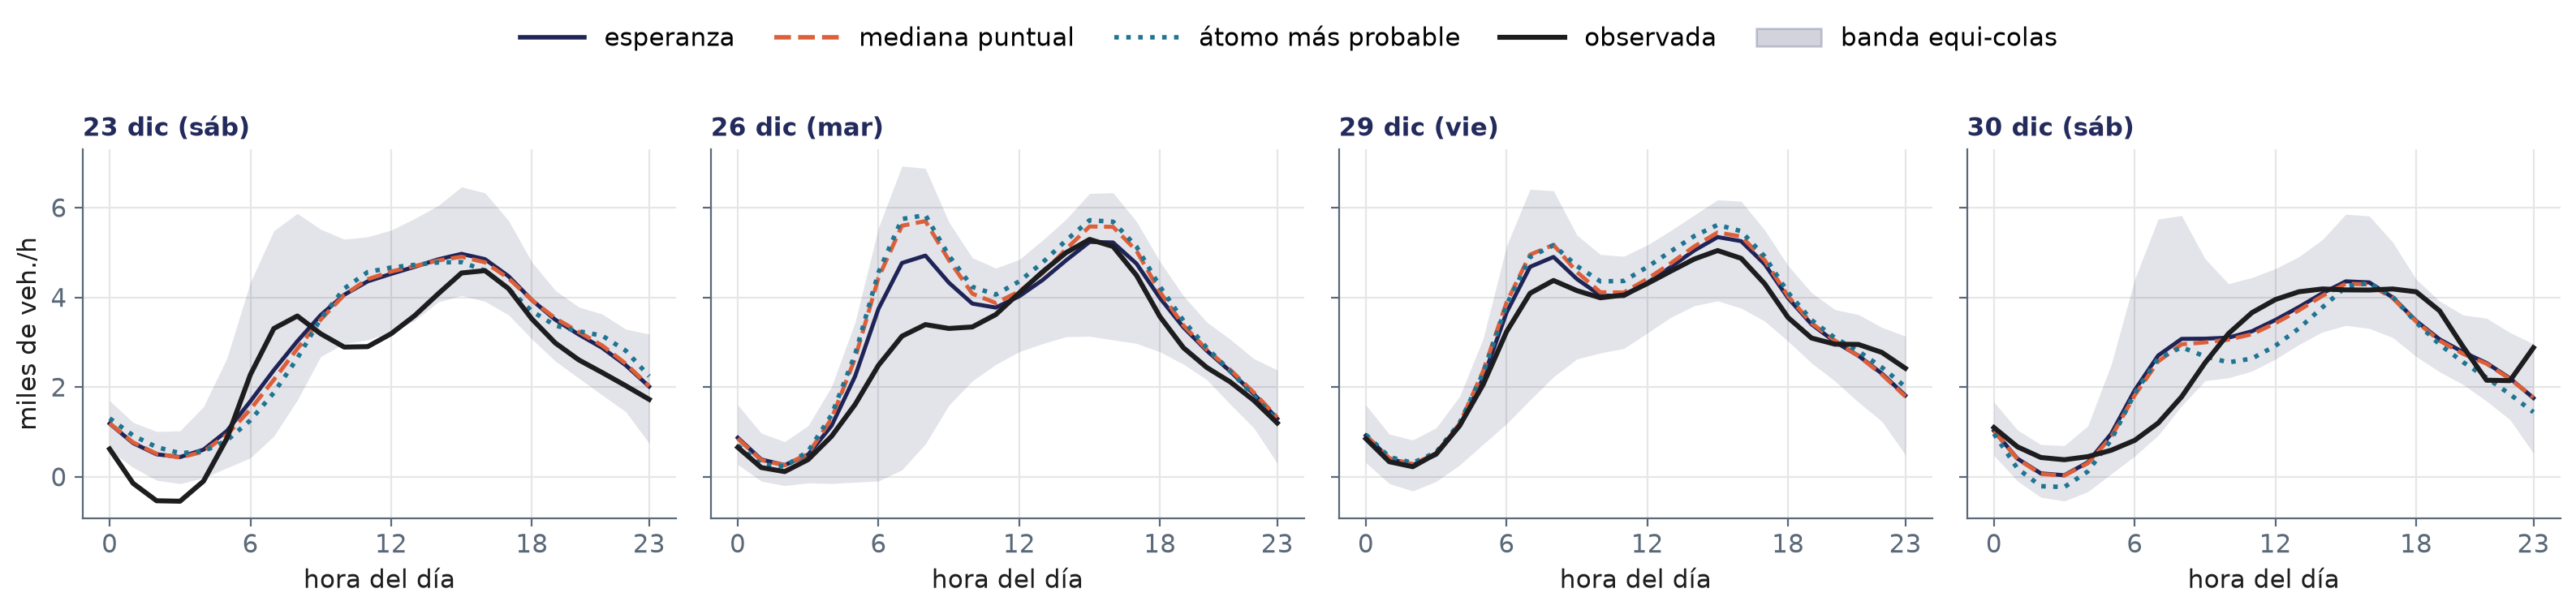
\includegraphics[width=\textwidth,height=0.8\textheight,keepaspectratio]{IMG/aneC_00/aneC_00_61b_curvas_predictores_102.png}
\caption{Curvas de los predictores puntuales en orígenes con más de un comportamiento, tráfico $\{1,7\}$ ($M = 10$).}
\label{fig:aneC_predictores_102}
\end{figure}

\begin{figure}[H]
\centering
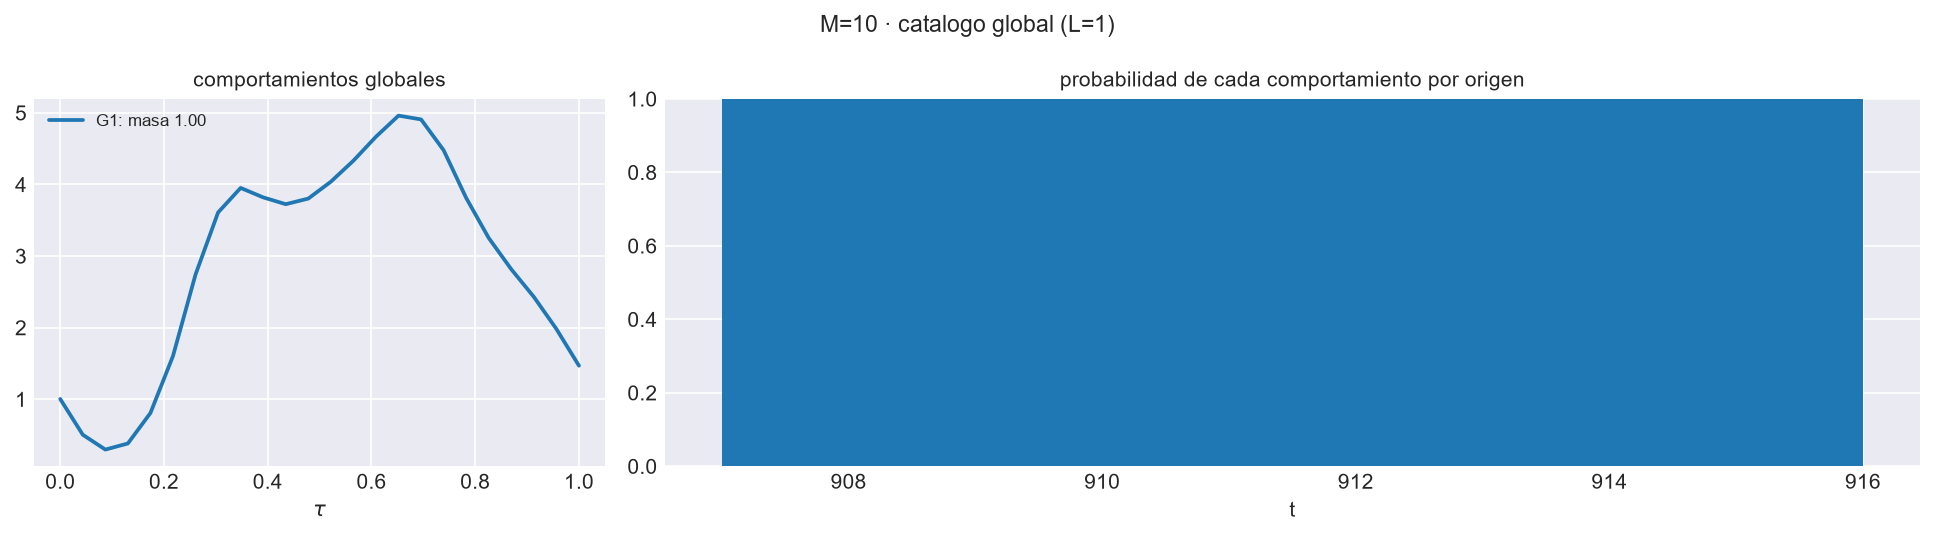
\includegraphics[width=\textwidth,height=0.6\textheight,keepaspectratio]{IMG/aneC_00/aneC_00_64_catalogo_global_102.png}
\caption{Catálogo global de comportamientos, tráfico $\{1,7\}$ ($M = 10$).}
\label{fig:aneC_catalogo_102}
\end{figure}

\begin{figure}[H]
\centering
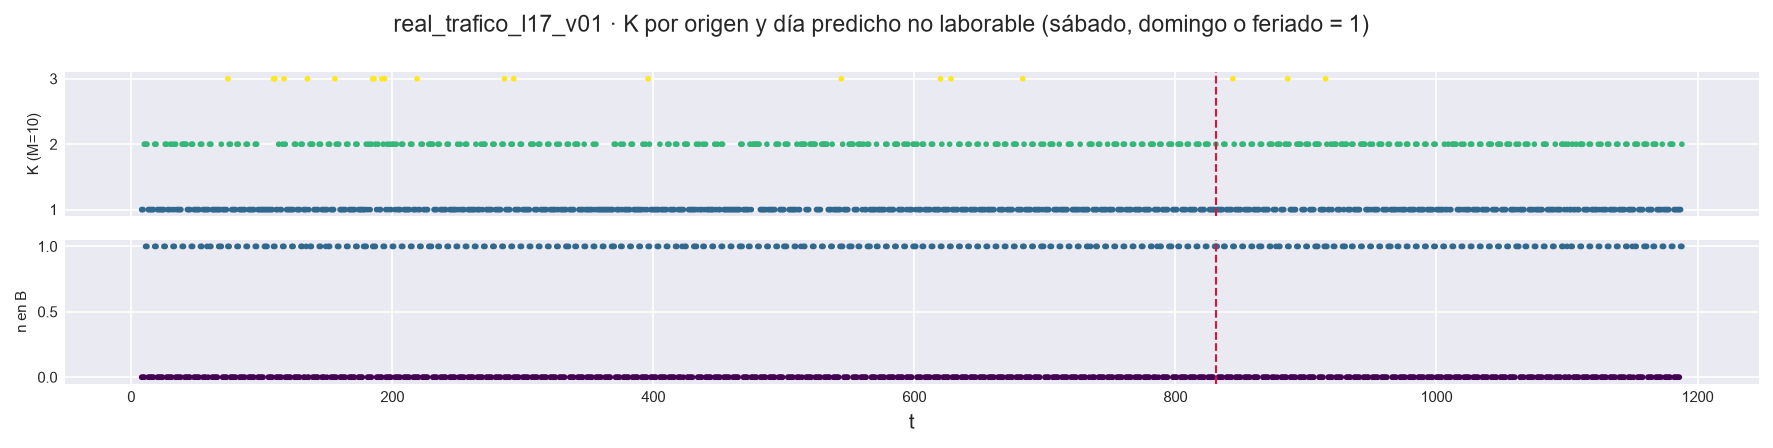
\includegraphics[width=\textwidth,height=0.6\textheight,keepaspectratio]{IMG/aneC_00/aneC_00_102b_K_serie_102.png}
\caption{Número de comportamientos $K_t$ a lo largo de la serie, tráfico $\{1,7\}$ ($M = 10$).}
\label{fig:aneC_Kserie_102}
\end{figure}

\begin{figure}[H]
\centering
\begin{minipage}{0.49\textwidth}\centering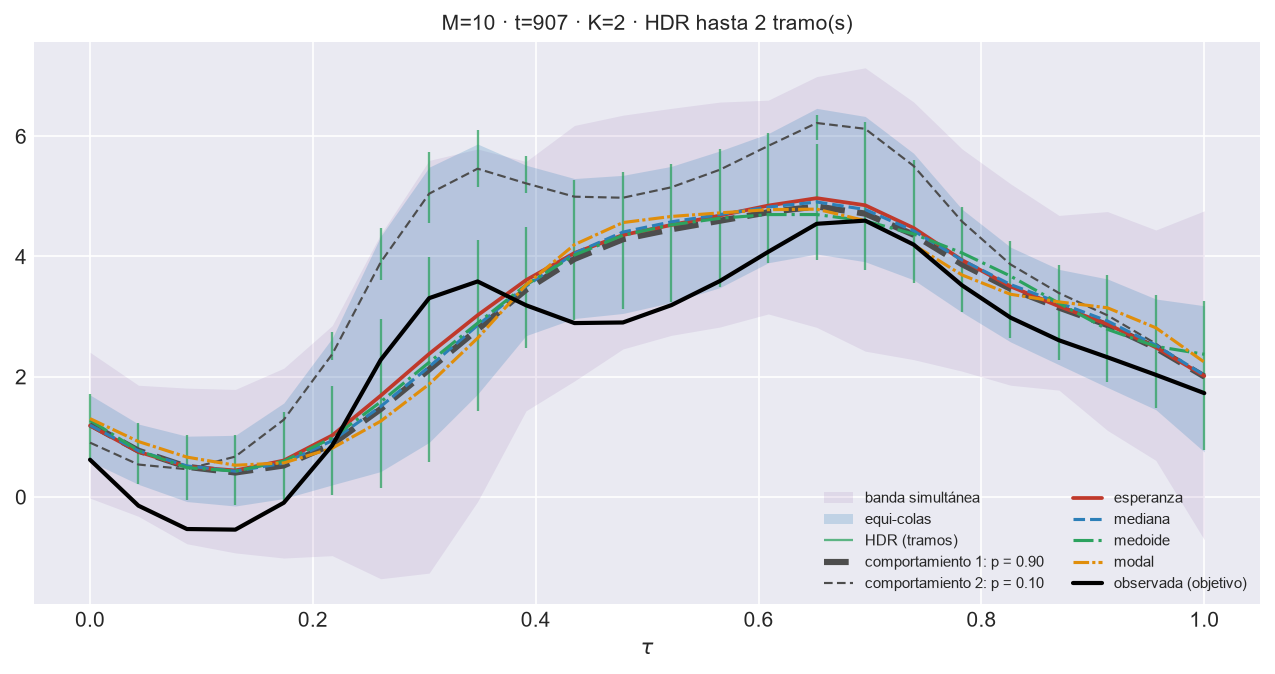
\includegraphics[width=\textwidth,height=0.4\textheight,keepaspectratio]{IMG/aneC_00/aneC_00_63_detalle_t907_102.png}\end{minipage}\hfill
\begin{minipage}{0.49\textwidth}\centering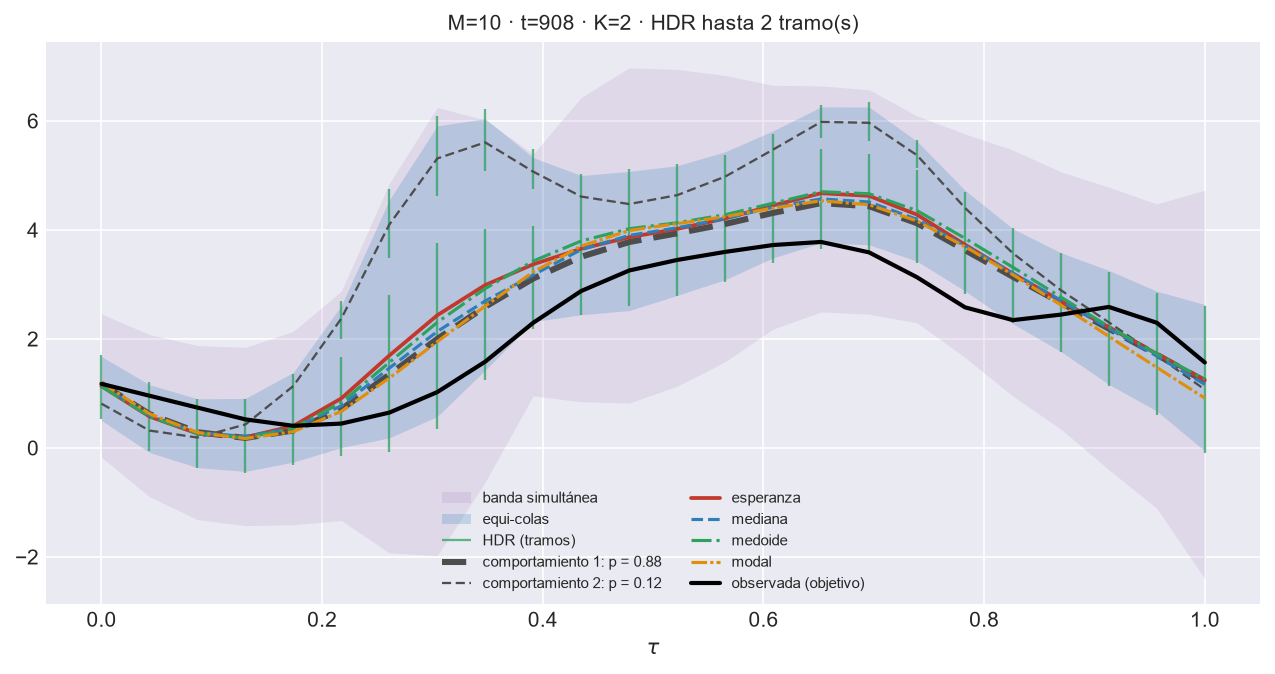
\includegraphics[width=\textwidth,height=0.4\textheight,keepaspectratio]{IMG/aneC_00/aneC_00_63_detalle_t908_102.png}\end{minipage}
\caption{Ventana de detalle, tráfico $\{1,7\}$, orígenes $t = 907$ y $t = 908$ ($M = 10$).}
\label{fig:aneC_detalle_907_102}
\end{figure}

\begin{figure}[H]
\centering
\begin{minipage}{0.49\textwidth}\centering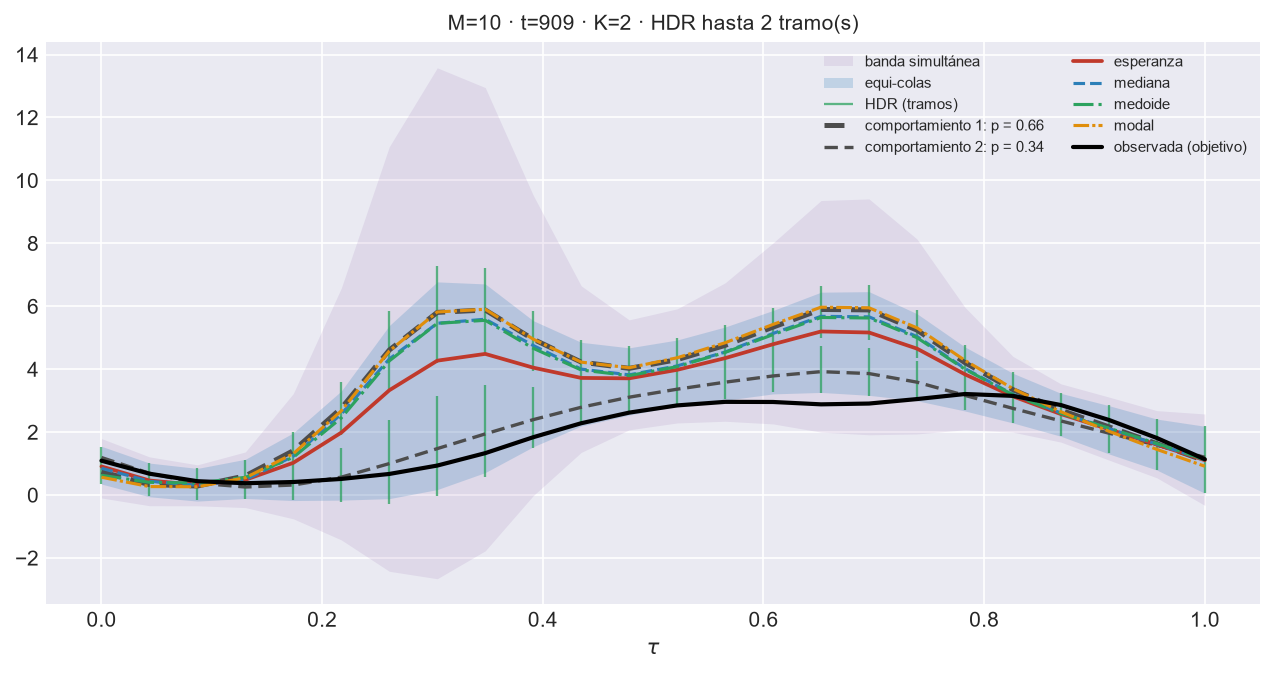
\includegraphics[width=\textwidth,height=0.4\textheight,keepaspectratio]{IMG/aneC_00/aneC_00_63_detalle_t909_102.png}\end{minipage}\hfill
\begin{minipage}{0.49\textwidth}\centering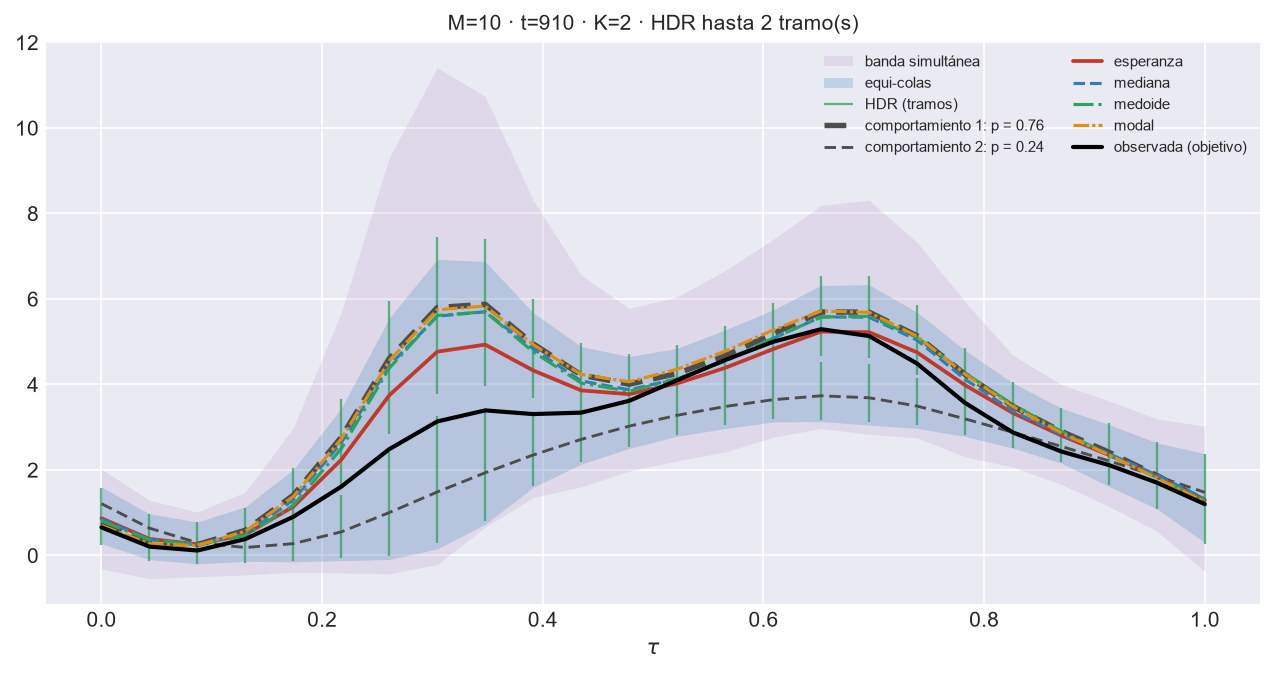
\includegraphics[width=\textwidth,height=0.4\textheight,keepaspectratio]{IMG/aneC_00/aneC_00_63_detalle_t910_102.png}\end{minipage}
\caption{Ventana de detalle, tráfico $\{1,7\}$, orígenes $t = 909$ y $t = 910$ ($M = 10$).}
\label{fig:aneC_detalle_909_102}
\end{figure}

\begin{figure}[H]
\centering
\begin{minipage}{0.49\textwidth}\centering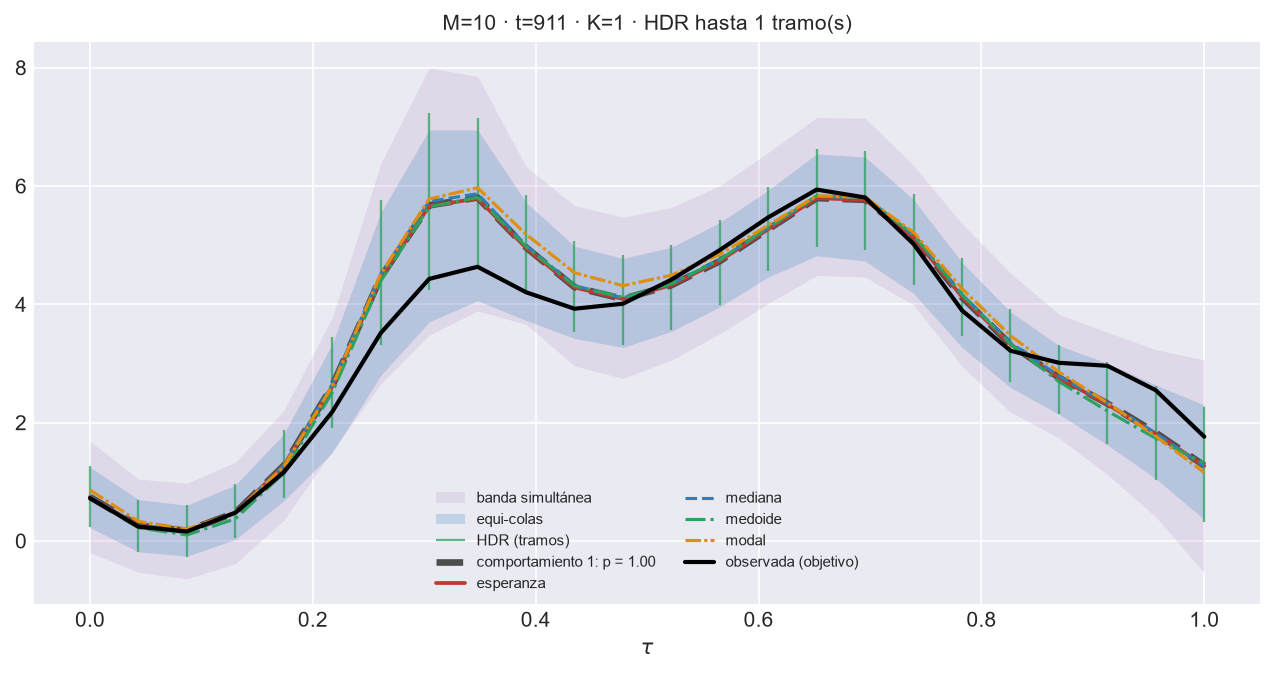
\includegraphics[width=\textwidth,height=0.4\textheight,keepaspectratio]{IMG/aneC_00/aneC_00_63_detalle_t911_102.png}\end{minipage}\hfill
\begin{minipage}{0.49\textwidth}\centering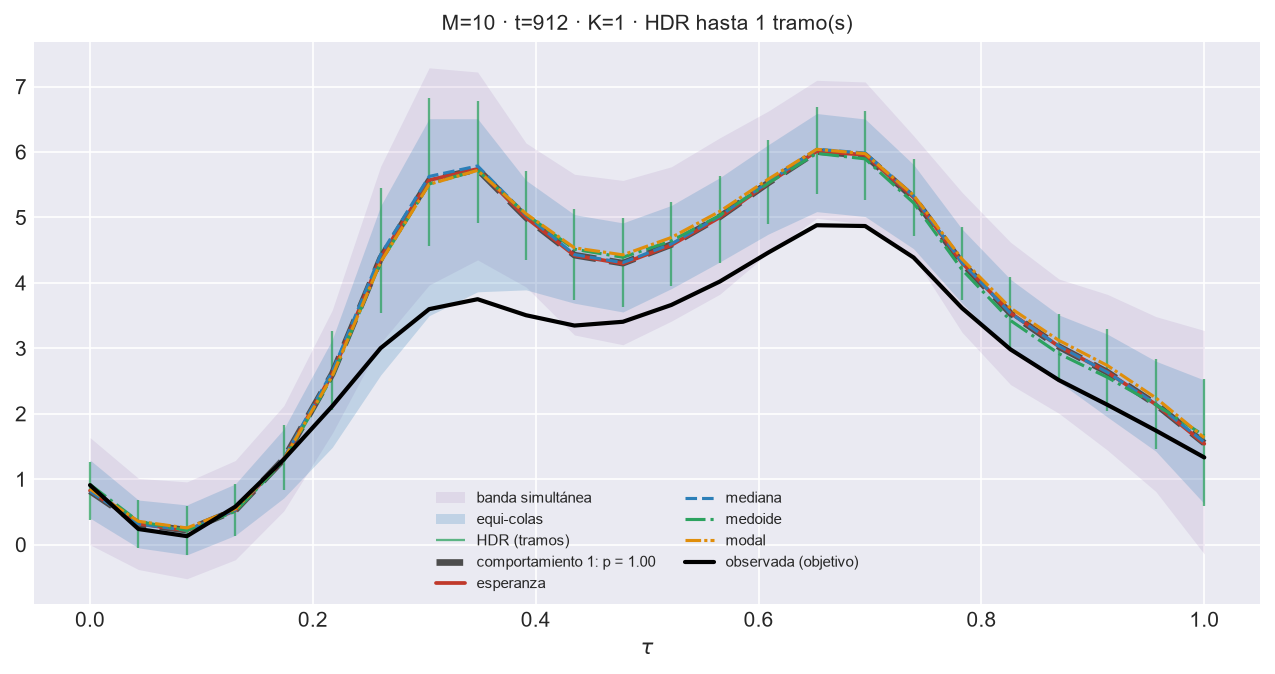
\includegraphics[width=\textwidth,height=0.4\textheight,keepaspectratio]{IMG/aneC_00/aneC_00_63_detalle_t912_102.png}\end{minipage}
\caption{Ventana de detalle, tráfico $\{1,7\}$, orígenes $t = 911$ y $t = 912$ ($M = 10$).}
\label{fig:aneC_detalle_911_102}
\end{figure}

\begin{figure}[H]
\centering
\begin{minipage}{0.49\textwidth}\centering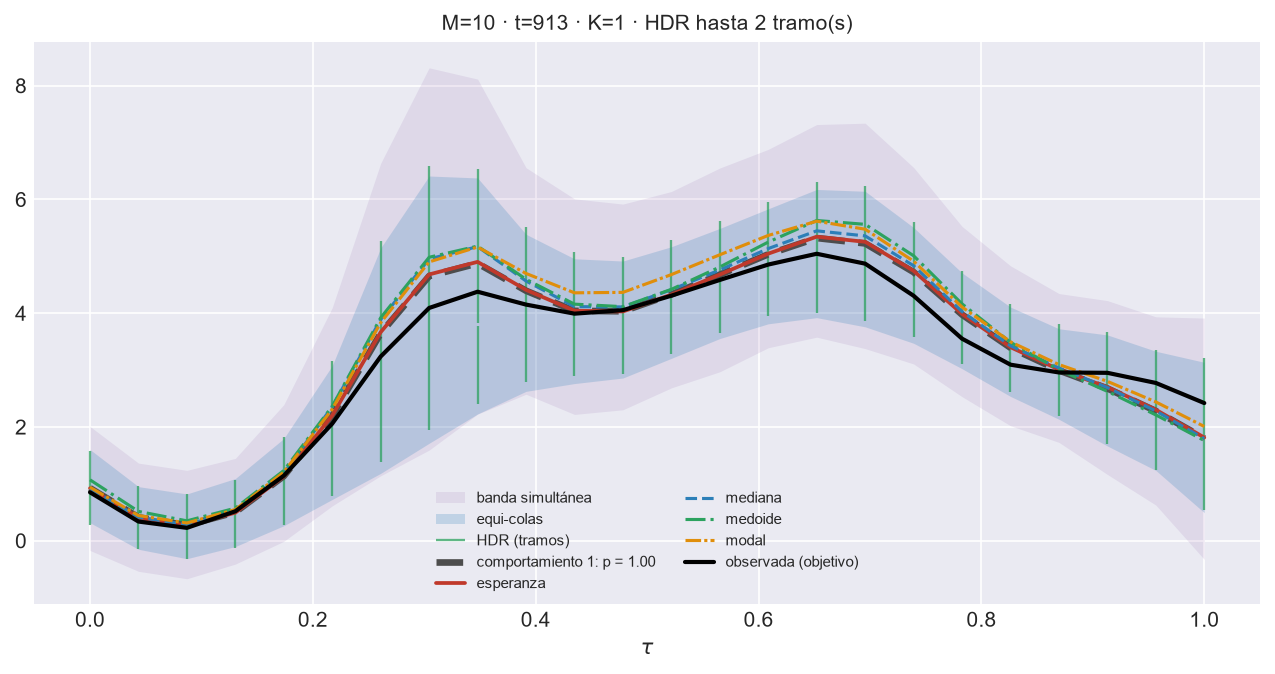
\includegraphics[width=\textwidth,height=0.4\textheight,keepaspectratio]{IMG/aneC_00/aneC_00_63_detalle_t913_102.png}\end{minipage}\hfill
\begin{minipage}{0.49\textwidth}\centering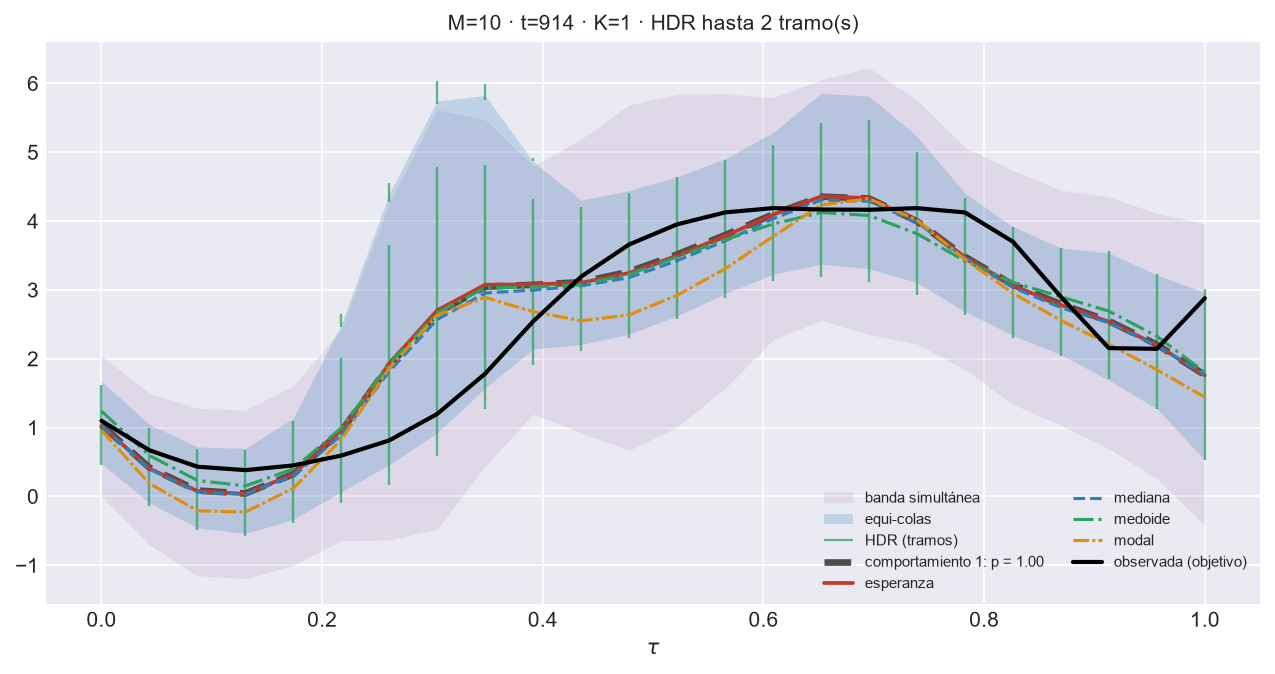
\includegraphics[width=\textwidth,height=0.4\textheight,keepaspectratio]{IMG/aneC_00/aneC_00_63_detalle_t914_102.png}\end{minipage}
\caption{Ventana de detalle, tráfico $\{1,7\}$, orígenes $t = 913$ y $t = 914$ ($M = 10$).}
\label{fig:aneC_detalle_913_102}
\end{figure}

\begin{figure}[H]
\centering
\begin{minipage}{0.49\textwidth}\centering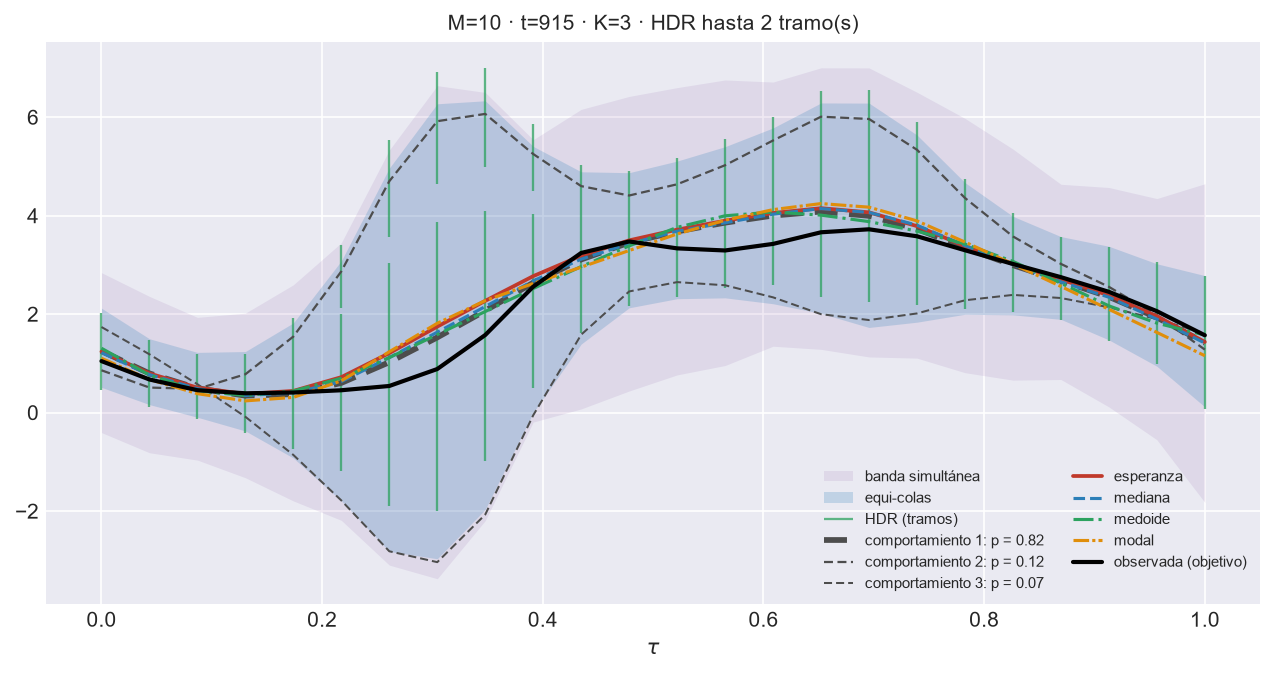
\includegraphics[width=\textwidth,height=0.4\textheight,keepaspectratio]{IMG/aneC_00/aneC_00_63_detalle_t915_102.png}\end{minipage}\hfill
\begin{minipage}{0.49\textwidth}\centering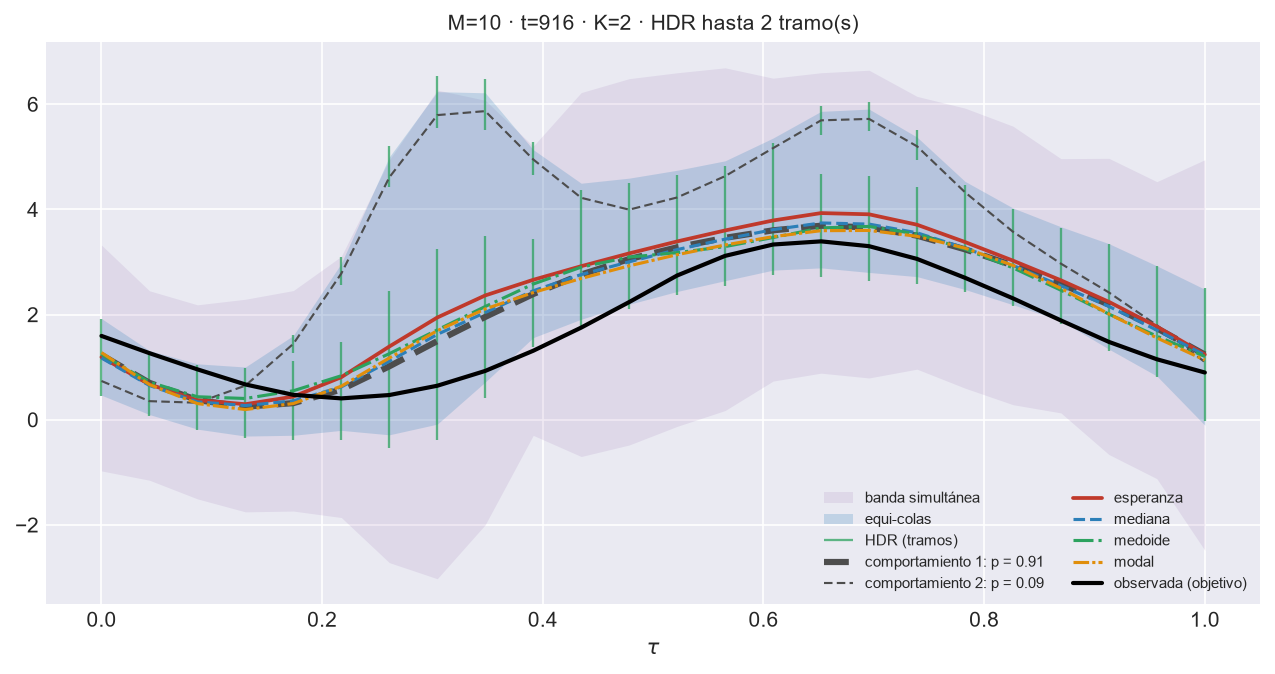
\includegraphics[width=\textwidth,height=0.4\textheight,keepaspectratio]{IMG/aneC_00/aneC_00_63_detalle_t916_102.png}\end{minipage}
\caption{Ventana de detalle, tráfico $\{1,7\}$, orígenes $t = 915$ y $t = 916$ ($M = 10$).}
\label{fig:aneC_detalle_915_102}
\end{figure}

\section{Intervalos curva a curva}
\label{aneC_00_05_intervalos_detalle}
% 79: contraste de las bandas en la ventana de detalle; 78: ganador por ventana del Bloque A.

\begin{figure}[H]
\centering
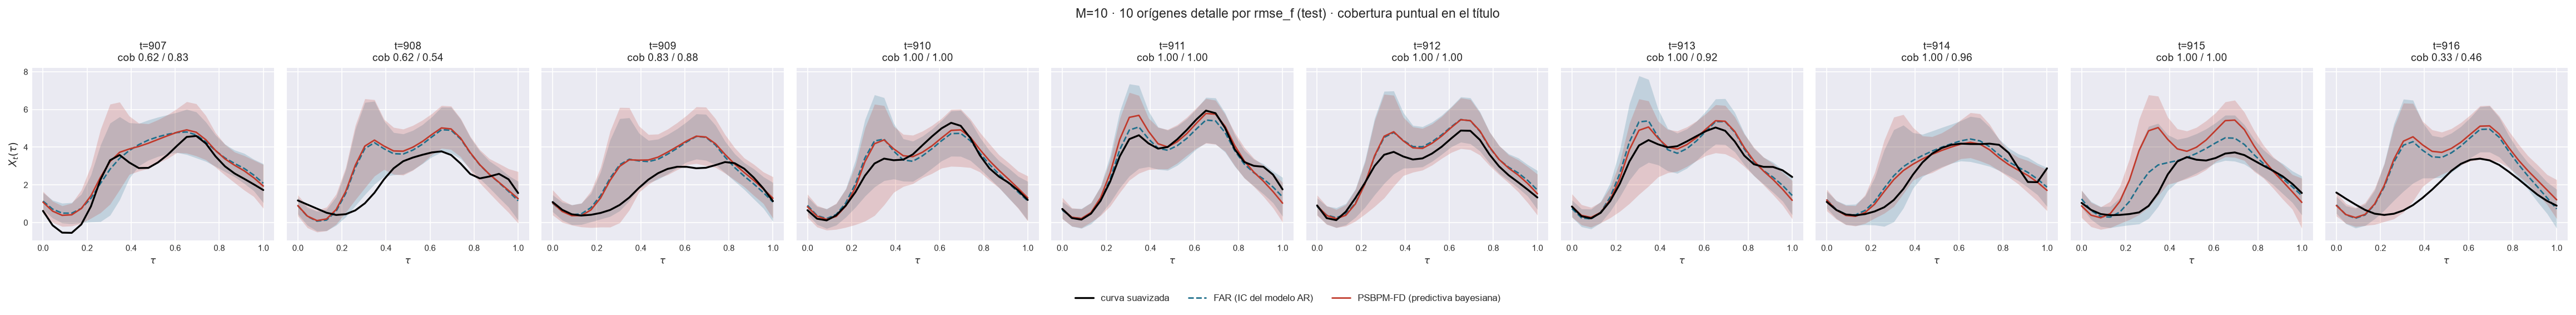
\includegraphics[width=\textwidth,height=0.75\textheight,keepaspectratio]{IMG/aneC_00/aneC_00_79_ic_contraste_detalle_101.png}
\caption{Bandas equi-colas y del FAR en la ventana de detalle, tráfico $\{1\}$ ($M = 10$).}
\label{fig:aneC_79_ic_contraste_detalle_101}
\end{figure}

\begin{figure}[H]
\centering
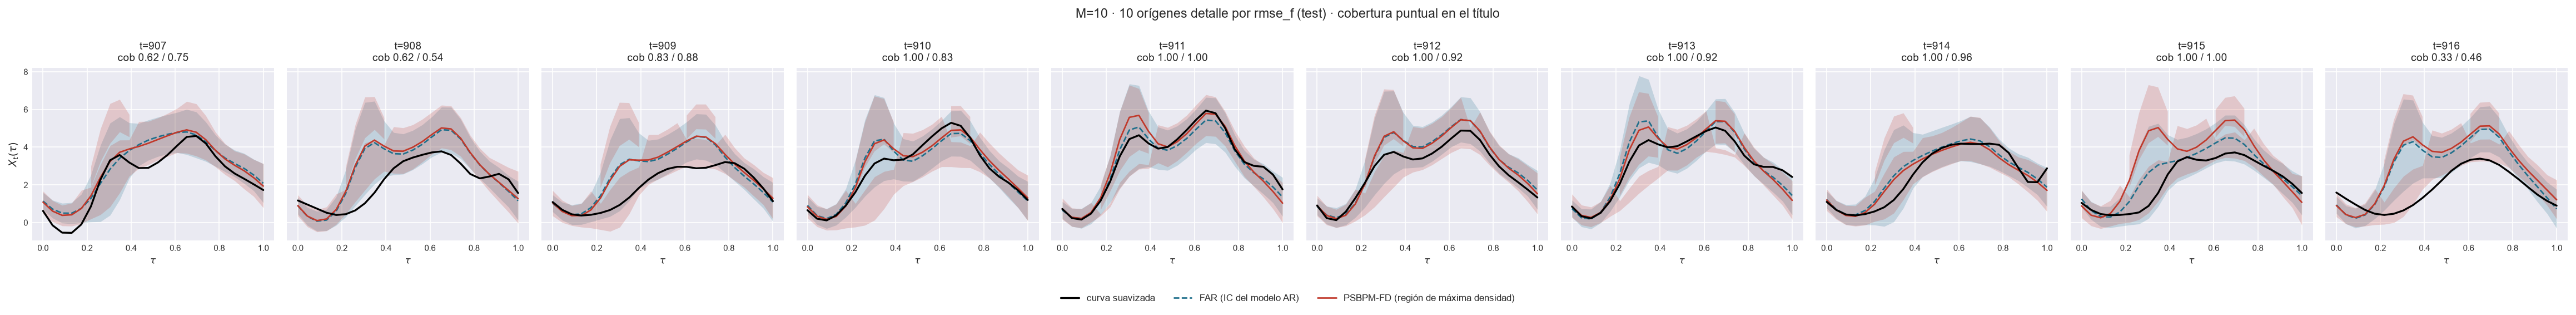
\includegraphics[width=\textwidth,height=0.75\textheight,keepaspectratio]{IMG/aneC_00/aneC_00_79_ic_contraste_detalle_hdr_101.png}
\caption{Banda de máxima densidad en la ventana de detalle, tráfico $\{1\}$ ($M = 10$).}
\label{fig:aneC_79_ic_contraste_detalle_hdr_101}
\end{figure}

\begin{figure}[H]
\centering
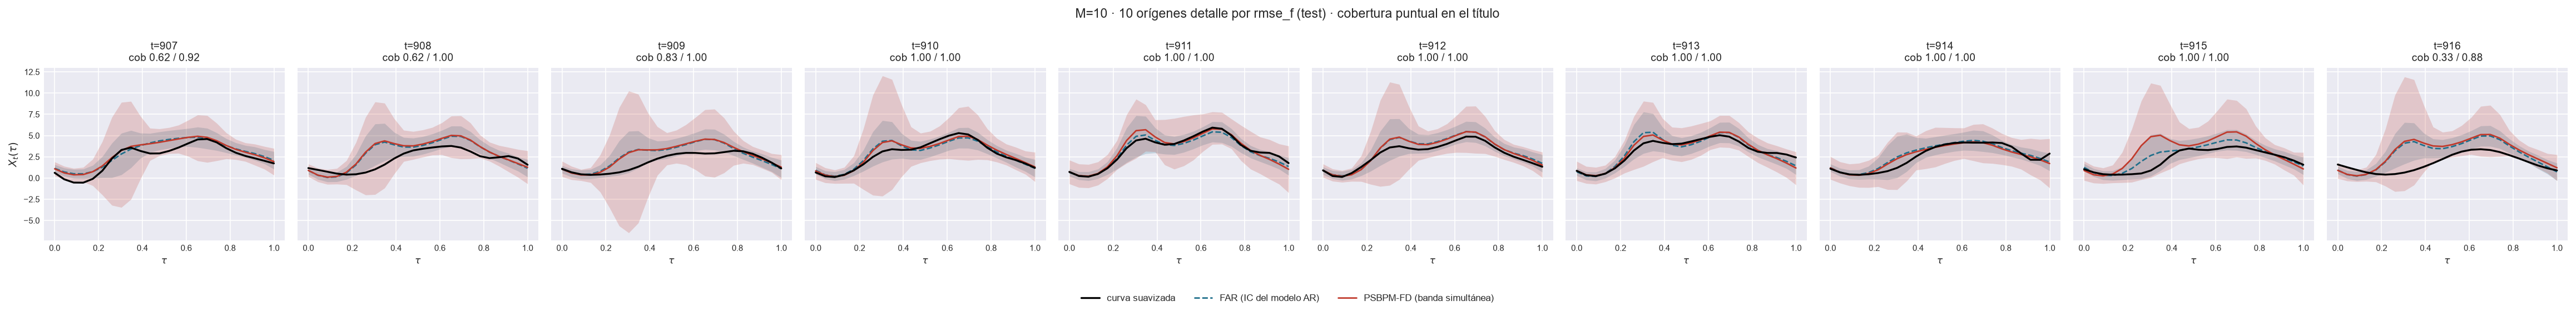
\includegraphics[width=\textwidth,height=0.75\textheight,keepaspectratio]{IMG/aneC_00/aneC_00_79_ic_contraste_detalle_simultanea_101.png}
\caption{Banda simultánea en la ventana de detalle, tráfico $\{1\}$ ($M = 10$).}
\label{fig:aneC_79_ic_contraste_detalle_simultanea_101}
\end{figure}

\begin{figure}[H]
\centering
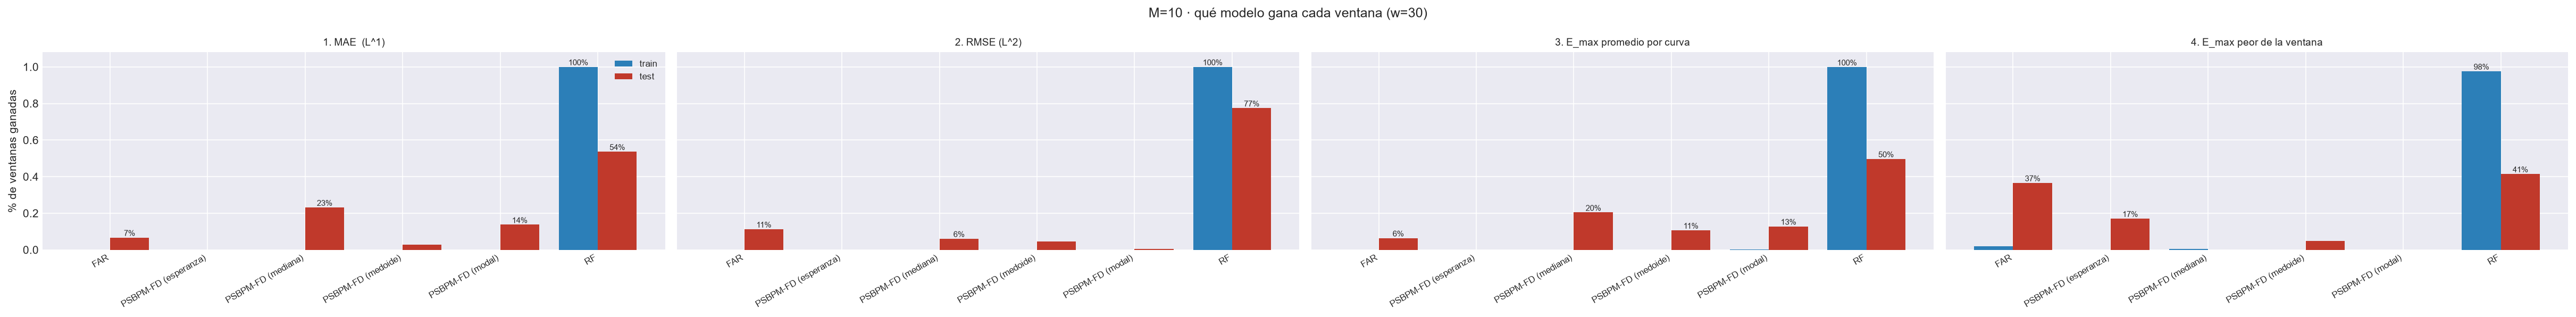
\includegraphics[width=\textwidth,height=0.75\textheight,keepaspectratio]{IMG/aneC_00/aneC_00_78_ganador_ventana_bloqueA_101.png}
\caption{Modelo ganador en cada ventana del bloque de prueba (MAE), tráfico $\{1\}$ ($M = 10$).}
\label{fig:aneC_78_ganador_ventana_bloqueA_101}
\end{figure}

\begin{figure}[H]
\centering
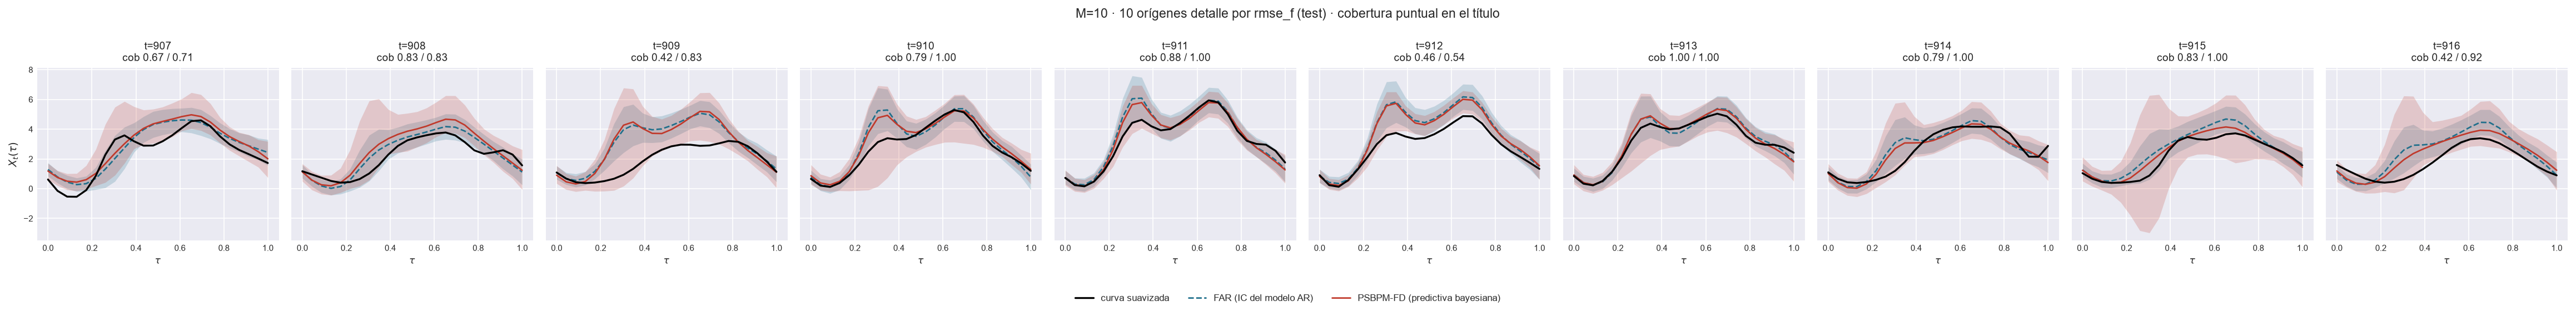
\includegraphics[width=\textwidth,height=0.75\textheight,keepaspectratio]{IMG/aneC_00/aneC_00_79_ic_contraste_detalle_102.png}
\caption{Bandas equi-colas y del FAR en la ventana de detalle, tráfico $\{1,7\}$ ($M = 10$).}
\label{fig:aneC_79_ic_contraste_detalle_102}
\end{figure}

\begin{figure}[H]
\centering
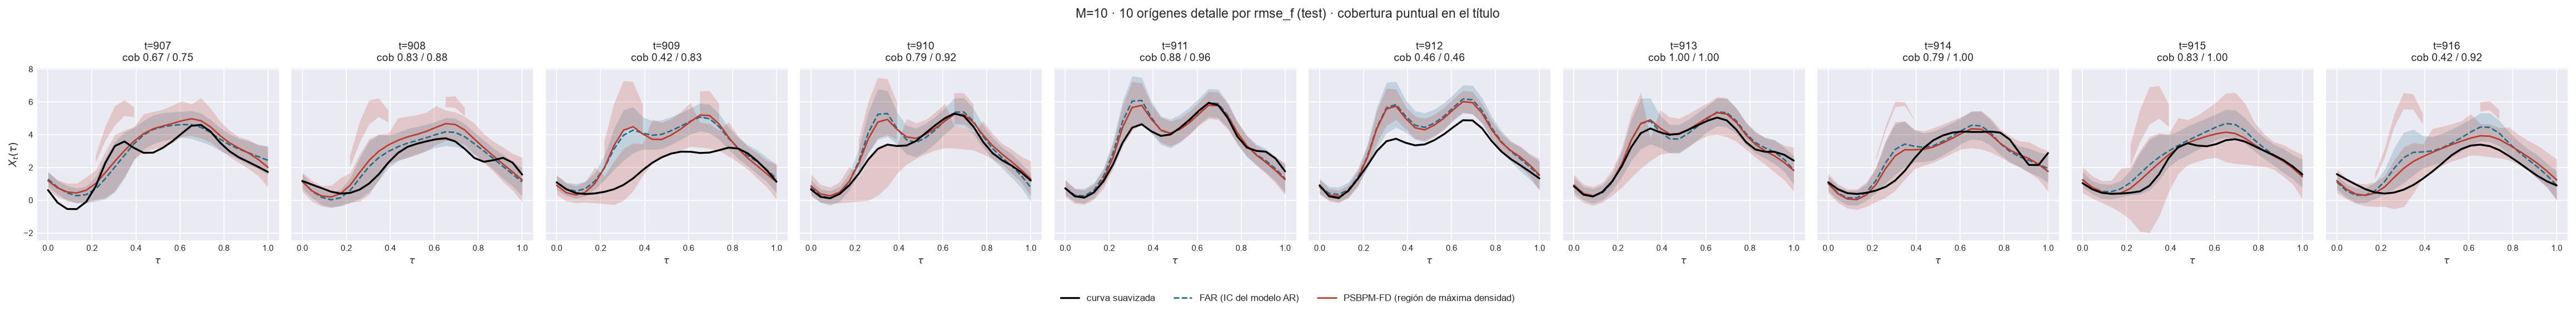
\includegraphics[width=\textwidth,height=0.75\textheight,keepaspectratio]{IMG/aneC_00/aneC_00_79_ic_contraste_detalle_hdr_102.png}
\caption{Banda de máxima densidad en la ventana de detalle, tráfico $\{1,7\}$ ($M = 10$).}
\label{fig:aneC_79_ic_contraste_detalle_hdr_102}
\end{figure}

\begin{figure}[H]
\centering
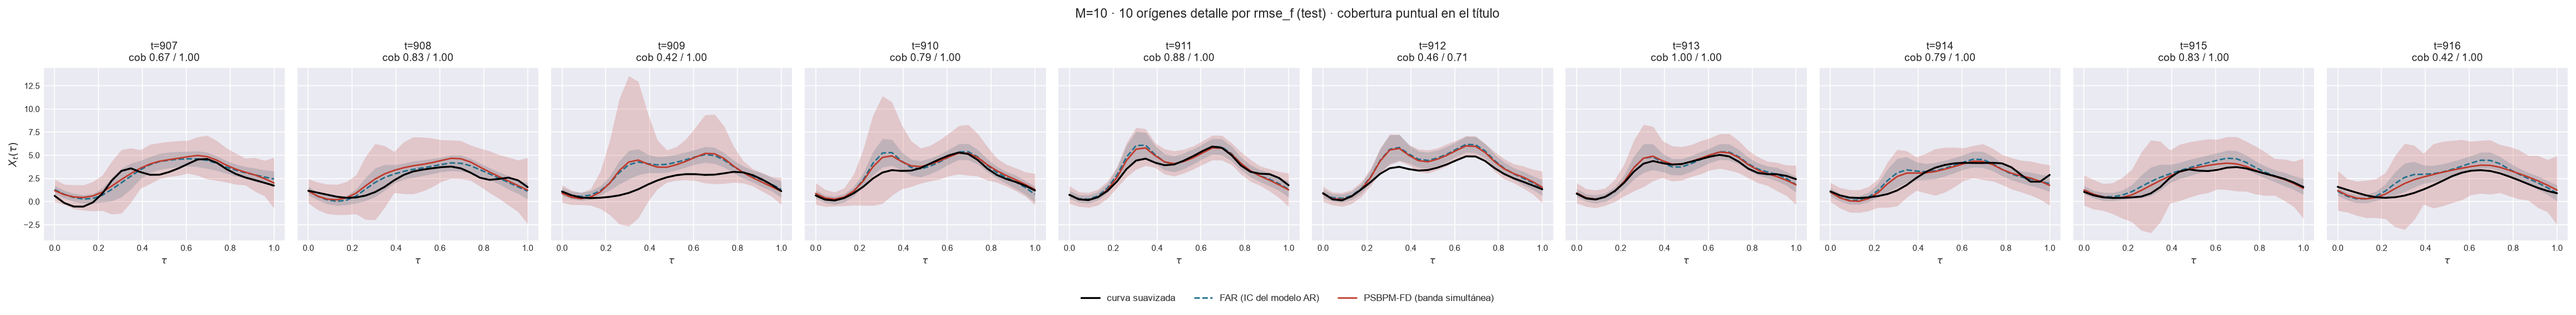
\includegraphics[width=\textwidth,height=0.75\textheight,keepaspectratio]{IMG/aneC_00/aneC_00_79_ic_contraste_detalle_simultanea_102.png}
\caption{Banda simultánea en la ventana de detalle, tráfico $\{1,7\}$ ($M = 10$).}
\label{fig:aneC_79_ic_contraste_detalle_simultanea_102}
\end{figure}

\begin{figure}[H]
\centering
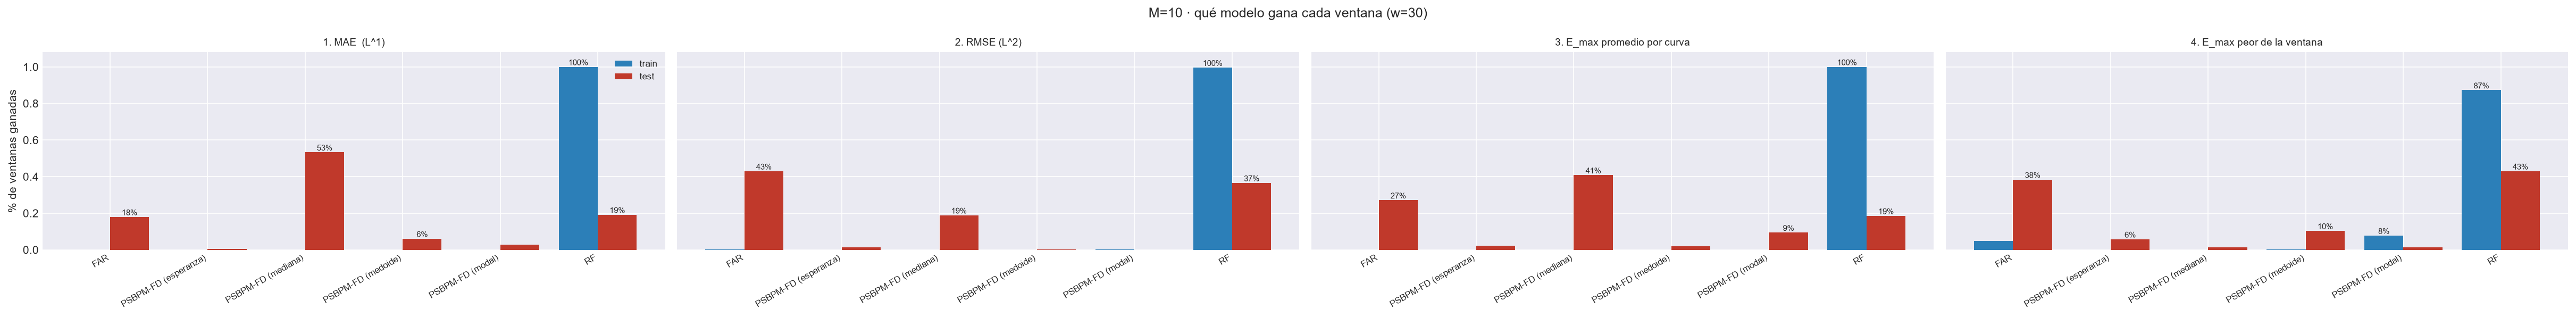
\includegraphics[width=\textwidth,height=0.75\textheight,keepaspectratio]{IMG/aneC_00/aneC_00_78_ganador_ventana_bloqueA_102.png}
\caption{Modelo ganador en cada ventana del bloque de prueba (MAE), tráfico $\{1,7\}$ ($M = 10$).}
\label{fig:aneC_78_ganador_ventana_bloqueA_102}
\end{figure}

\section{Monitoreo por componente}
\label{aneC_00_06_componentes}
% 91-94: error y banda de credibilidad de cada score, como en el Anexo B para simulación.

\begin{figure}[H]
\centering
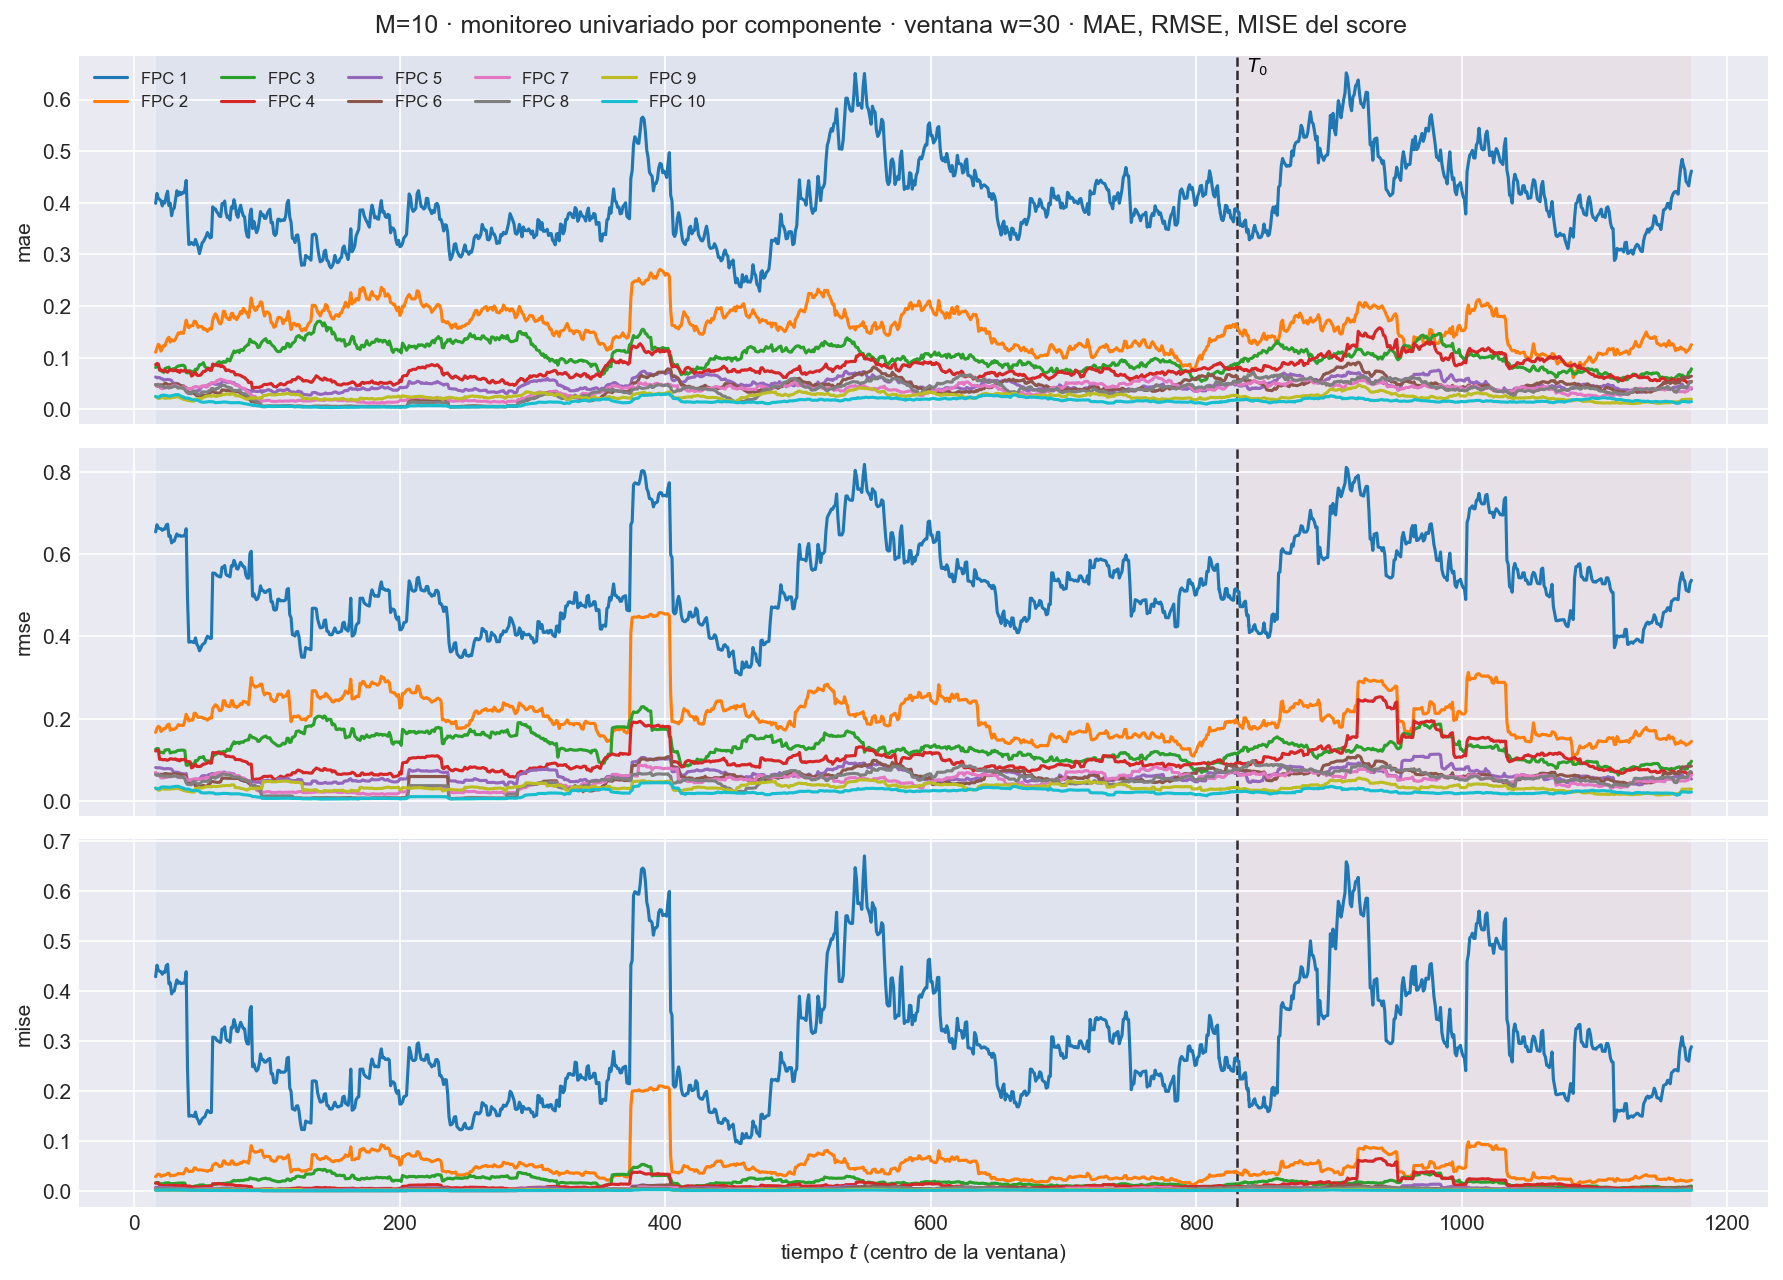
\includegraphics[width=\textwidth,height=0.75\textheight,keepaspectratio]{IMG/aneC_00/aneC_00_91_ventana_univariado_w30_101.png}
\caption{Error de cada score sobre la ventana móvil, tráfico $\{1\}$ ($M = 10$).}
\label{fig:aneC_91_ventana_univariado_w30_101}
\end{figure}

\begin{figure}[H]
\centering
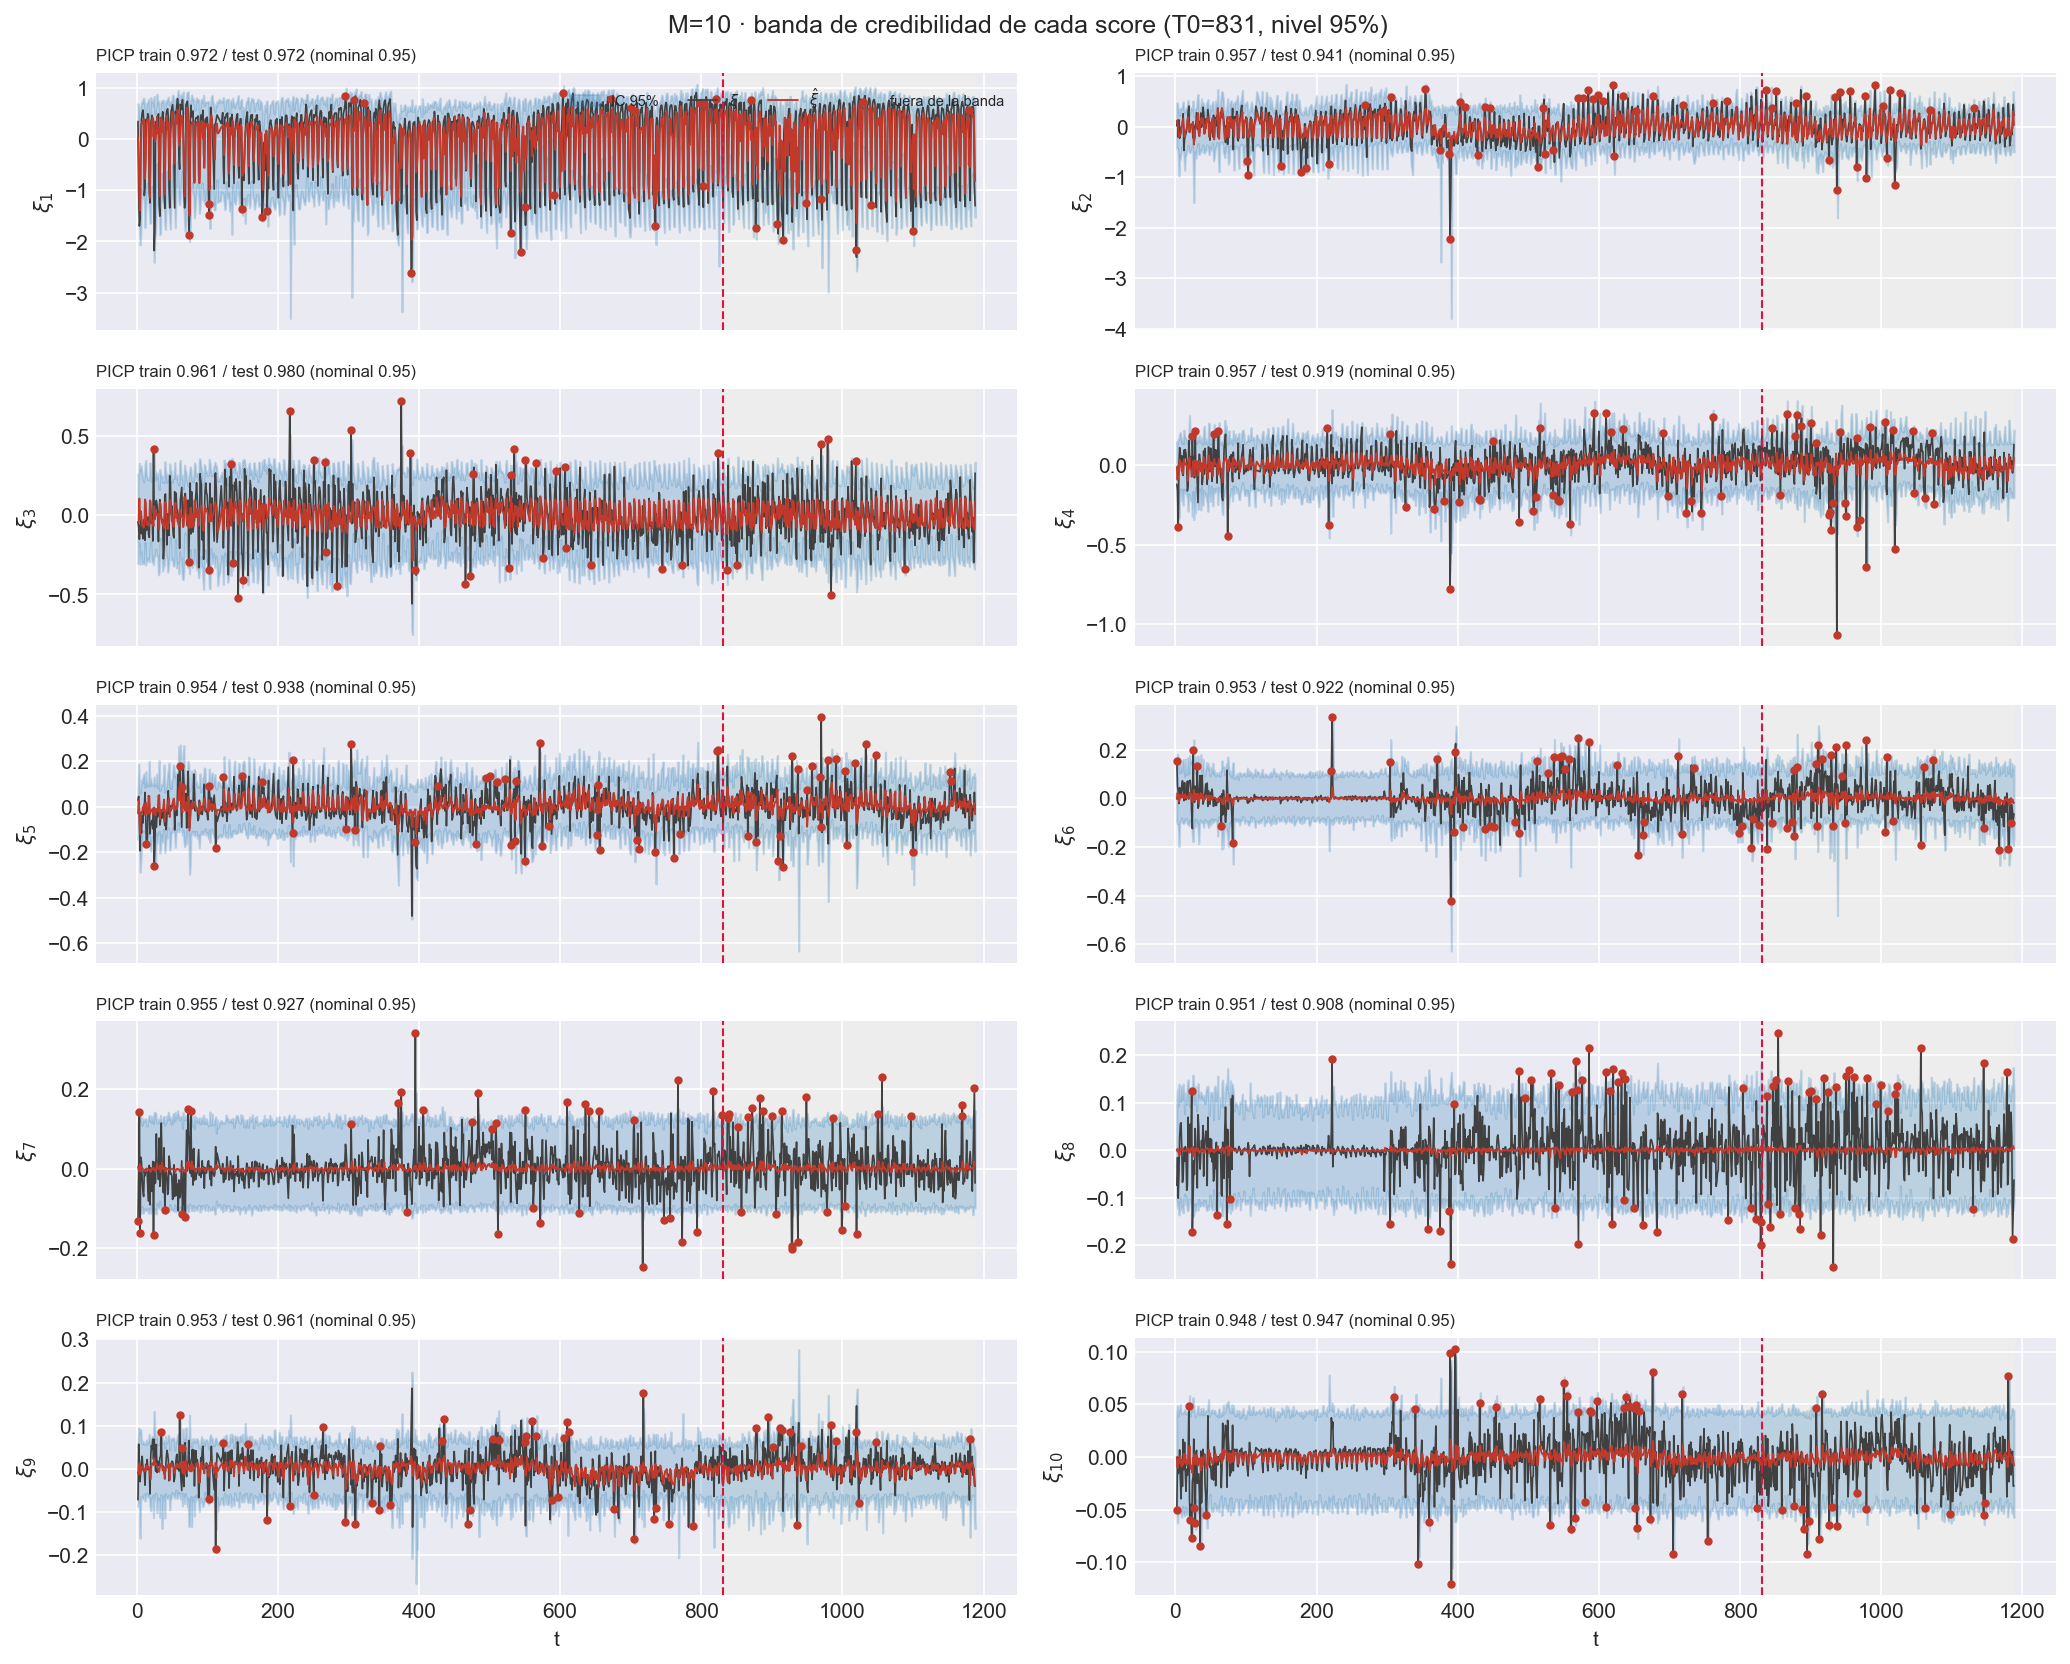
\includegraphics[width=\textwidth,height=0.75\textheight,keepaspectratio]{IMG/aneC_00/aneC_00_92_scores_banda_credibilidad_101.png}
\caption{Banda de credibilidad al 95\% de cada score, tráfico $\{1\}$ ($M = 10$).}
\label{fig:aneC_92_scores_banda_credibilidad_101}
\end{figure}

\begin{figure}[H]
\centering
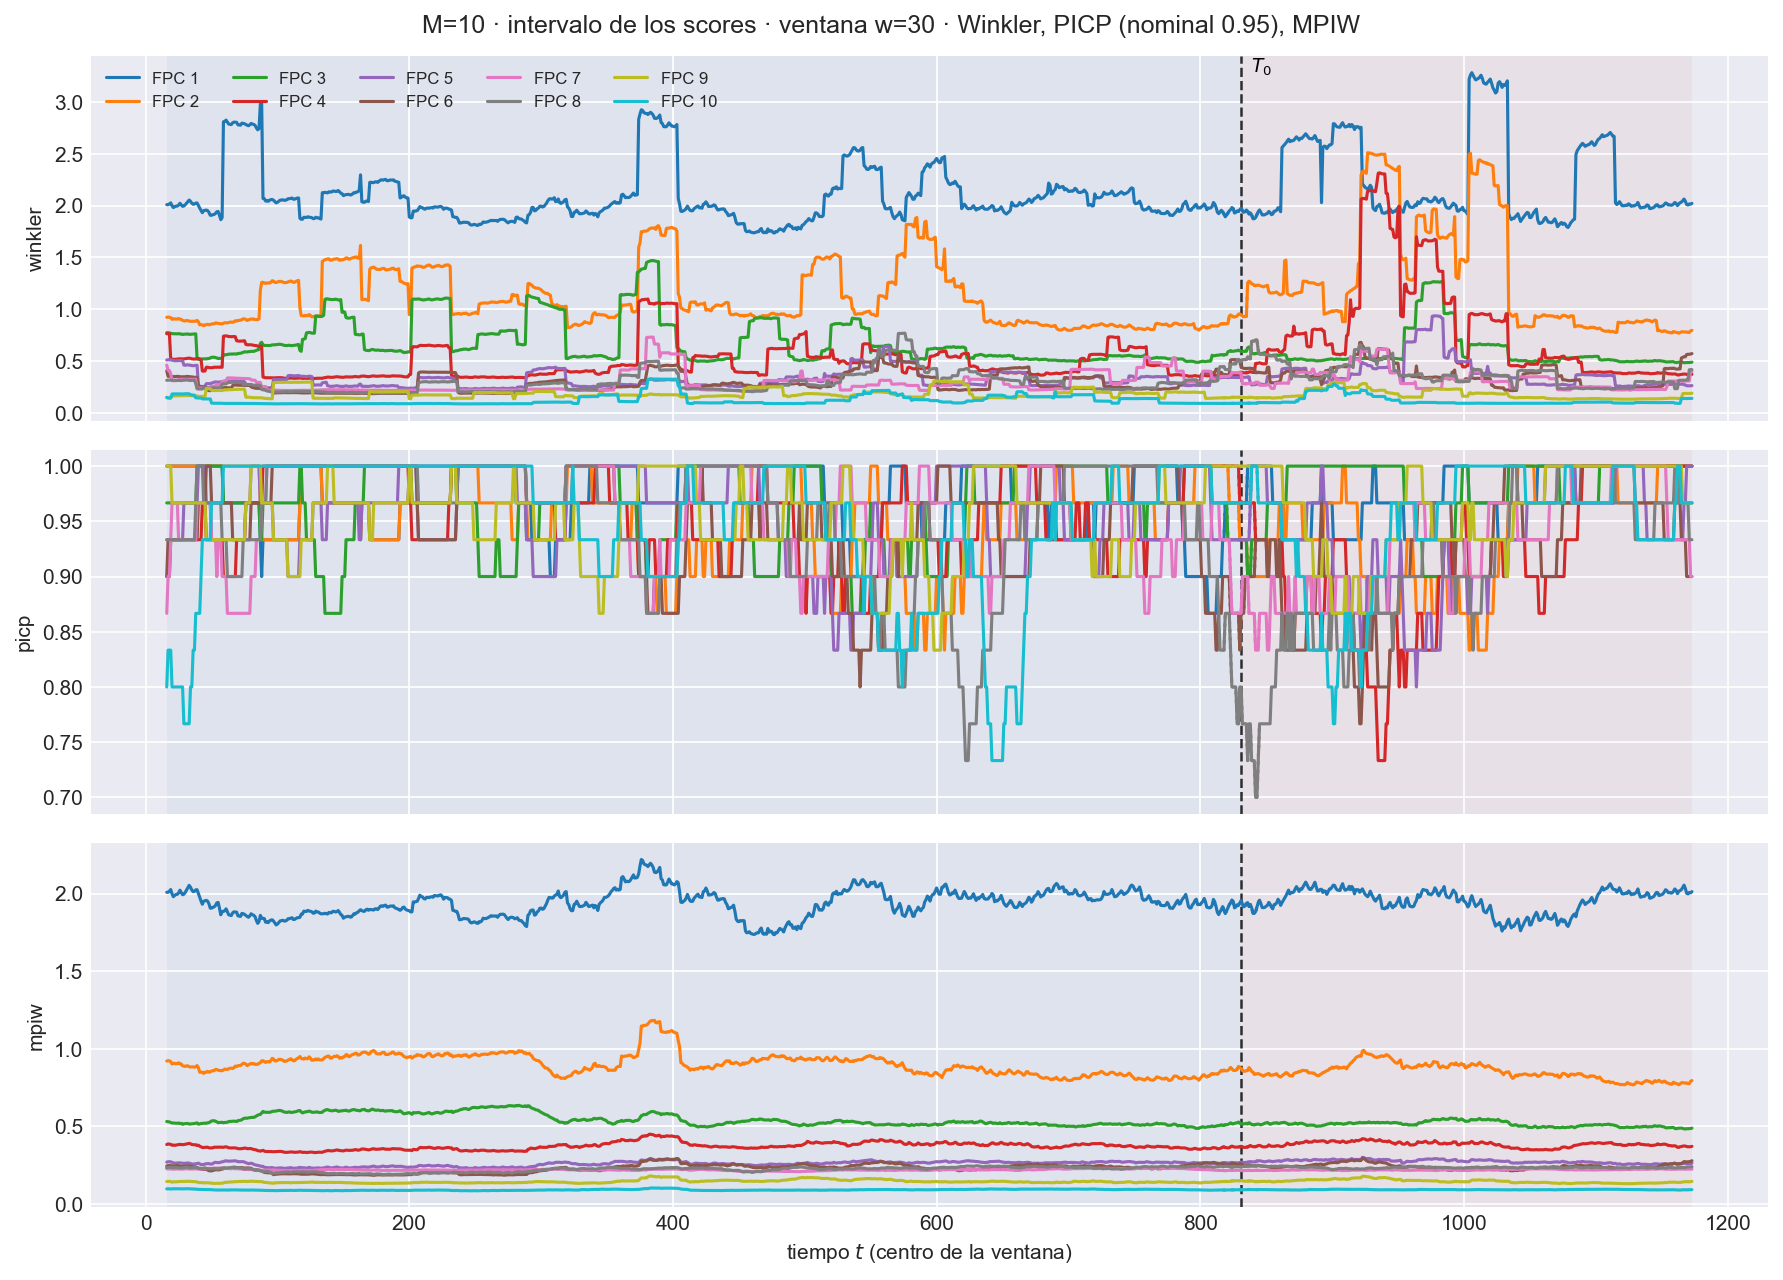
\includegraphics[width=\textwidth,height=0.75\textheight,keepaspectratio]{IMG/aneC_00/aneC_00_93_ventana_scores_intervalo_w30_101.png}
\caption{Métricas de intervalo de cada score sobre la ventana móvil, tráfico $\{1\}$ ($M = 10$).}
\label{fig:aneC_93_ventana_scores_intervalo_w30_101}
\end{figure}

\begin{figure}[H]
\centering
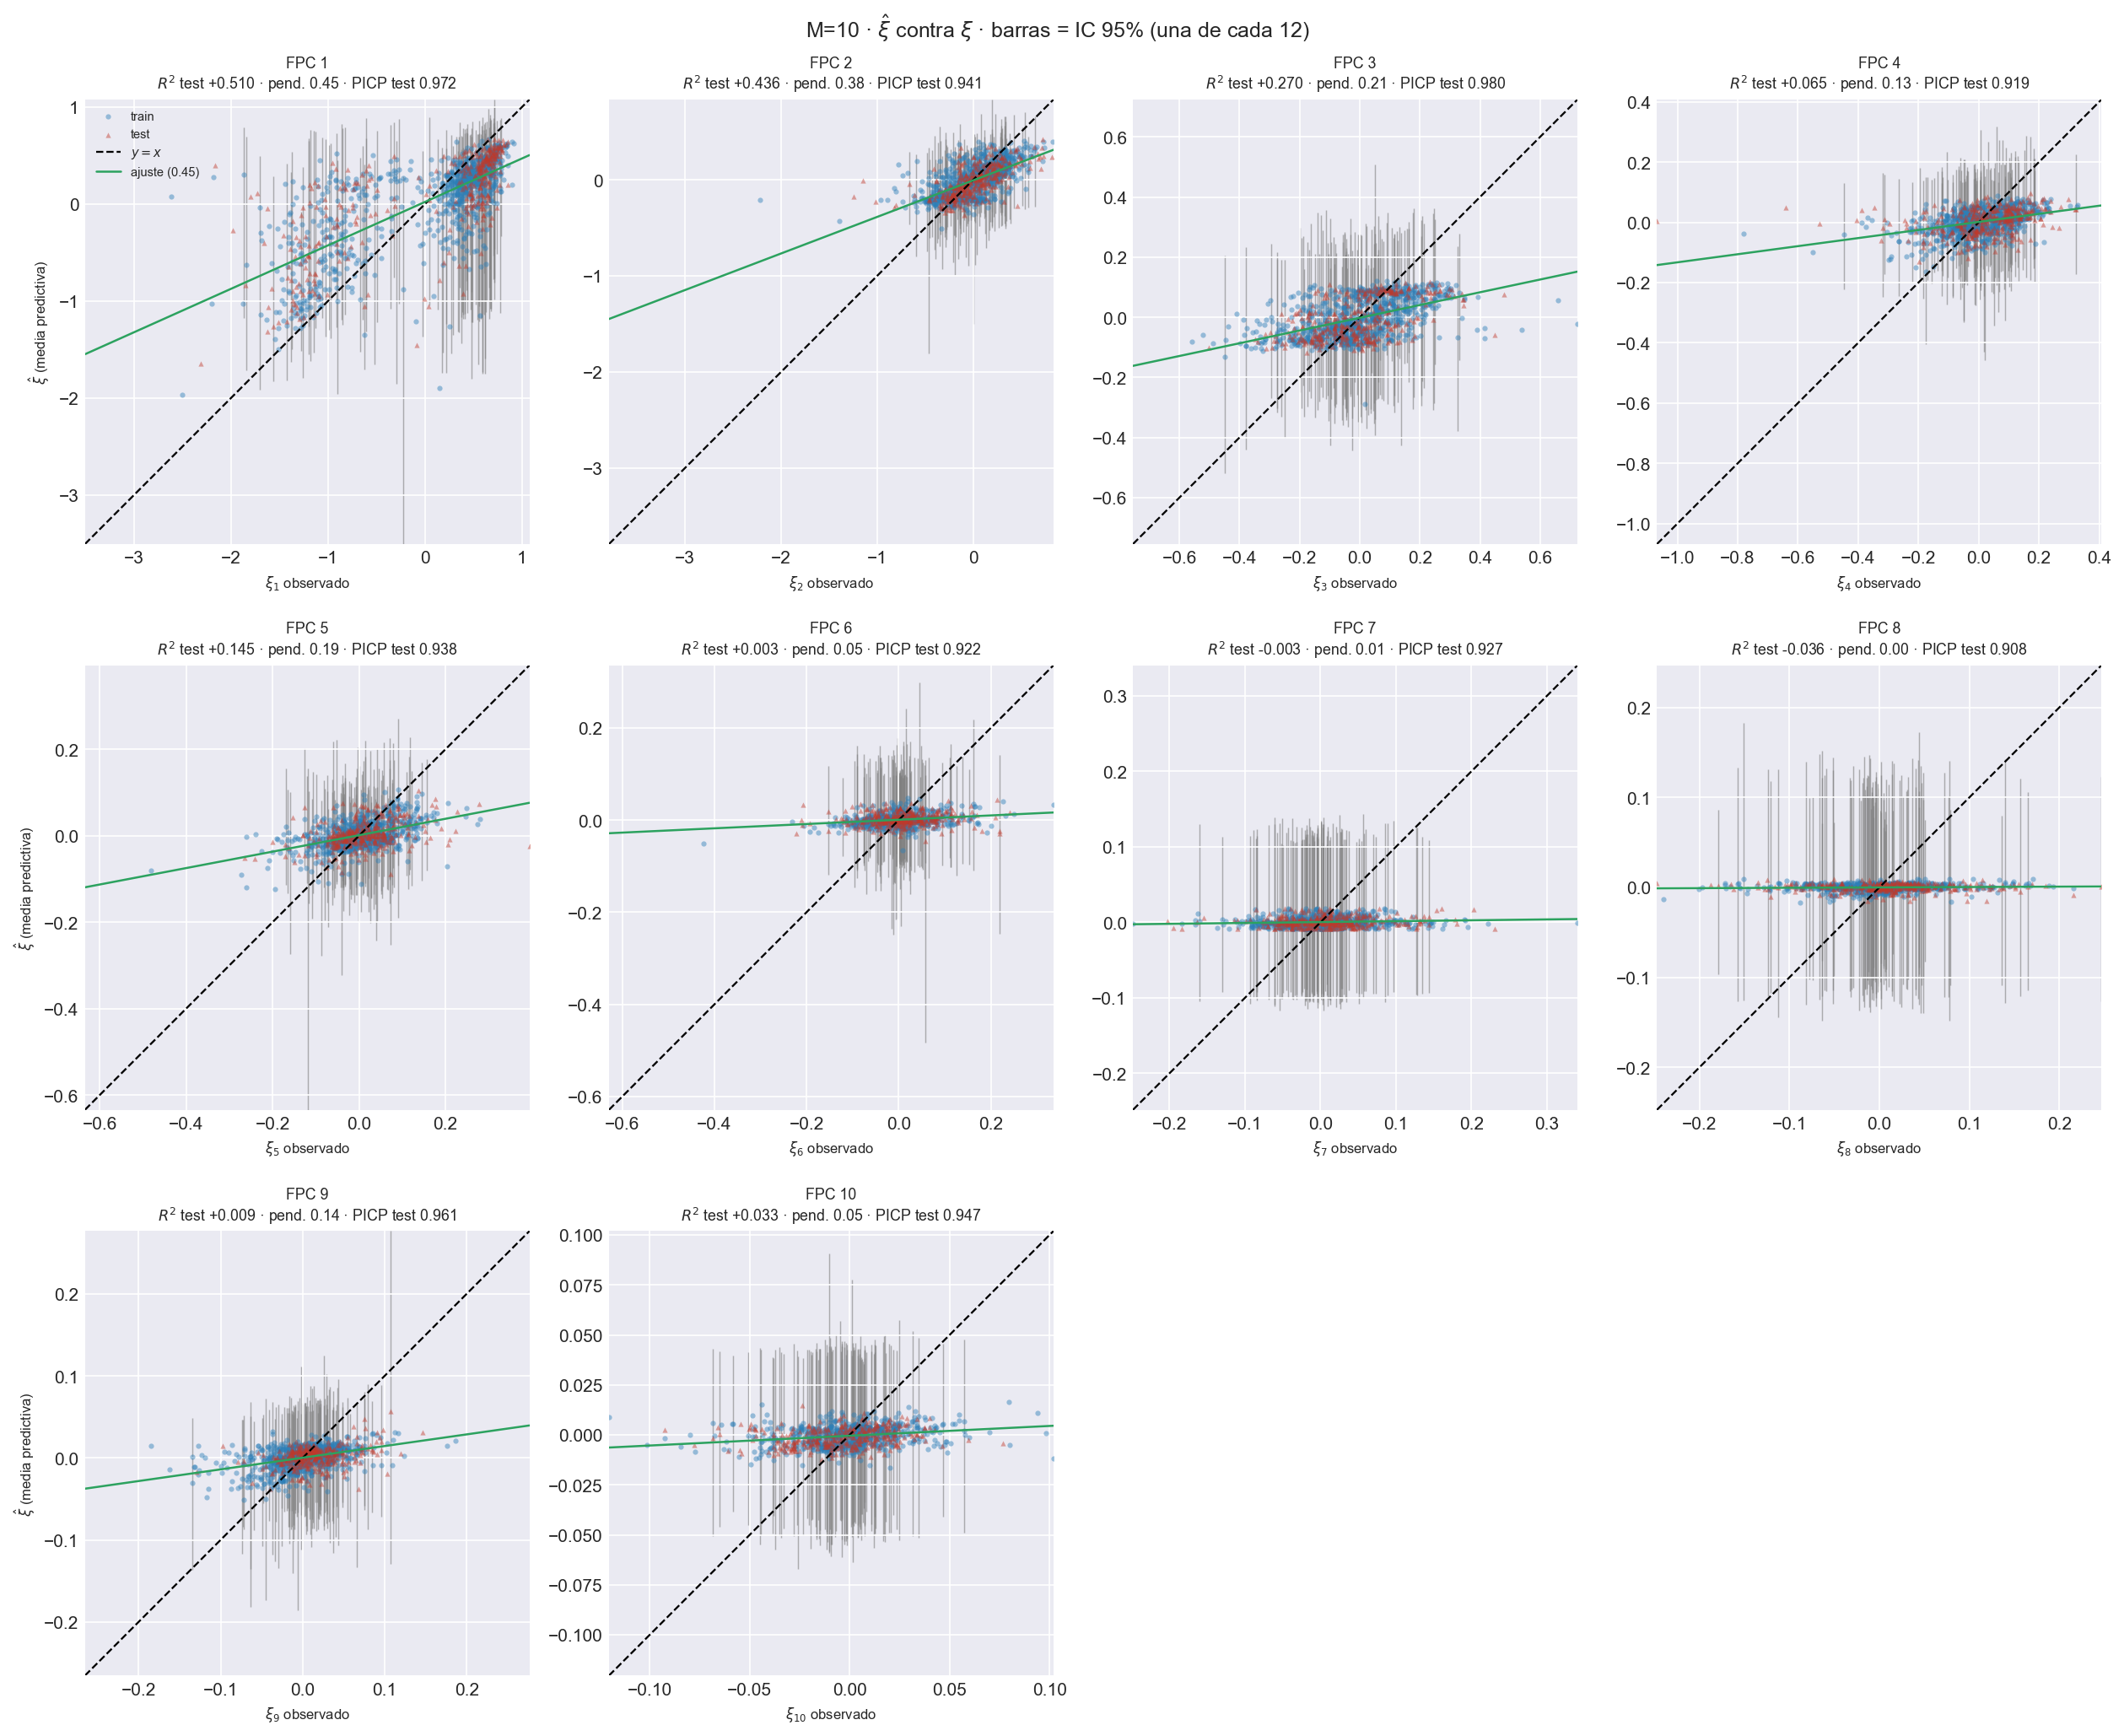
\includegraphics[width=\textwidth,height=0.75\textheight,keepaspectratio]{IMG/aneC_00/aneC_00_94_scores_dispersion_vs_real_101.png}
\caption{Dispersión estimada de cada score frente a la observada, tráfico $\{1\}$ ($M = 10$).}
\label{fig:aneC_94_scores_dispersion_vs_real_101}
\end{figure}

\begin{figure}[H]
\centering
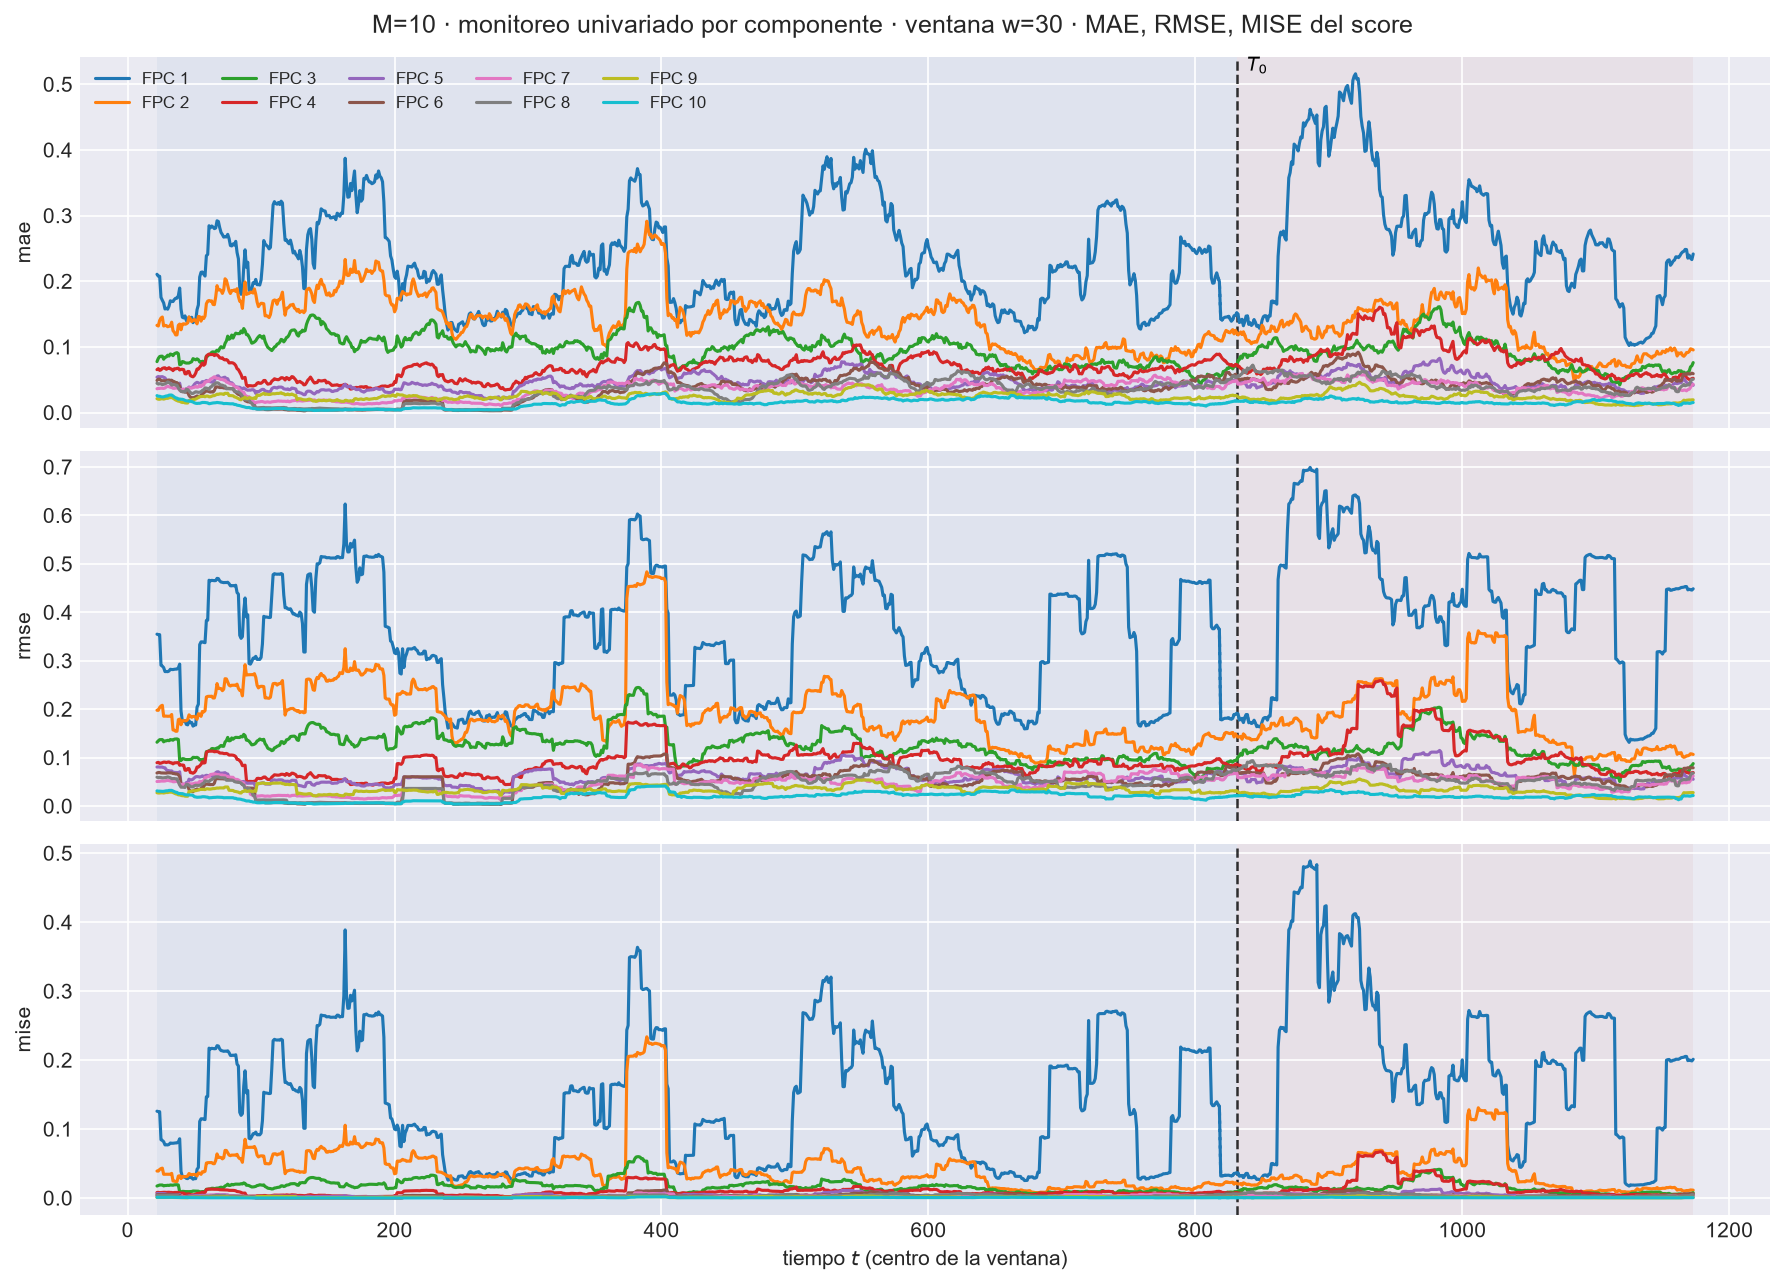
\includegraphics[width=\textwidth,height=0.75\textheight,keepaspectratio]{IMG/aneC_00/aneC_00_91_ventana_univariado_w30_102.png}
\caption{Error de cada score sobre la ventana móvil, tráfico $\{1,7\}$ ($M = 10$).}
\label{fig:aneC_91_ventana_univariado_w30_102}
\end{figure}

\begin{figure}[H]
\centering
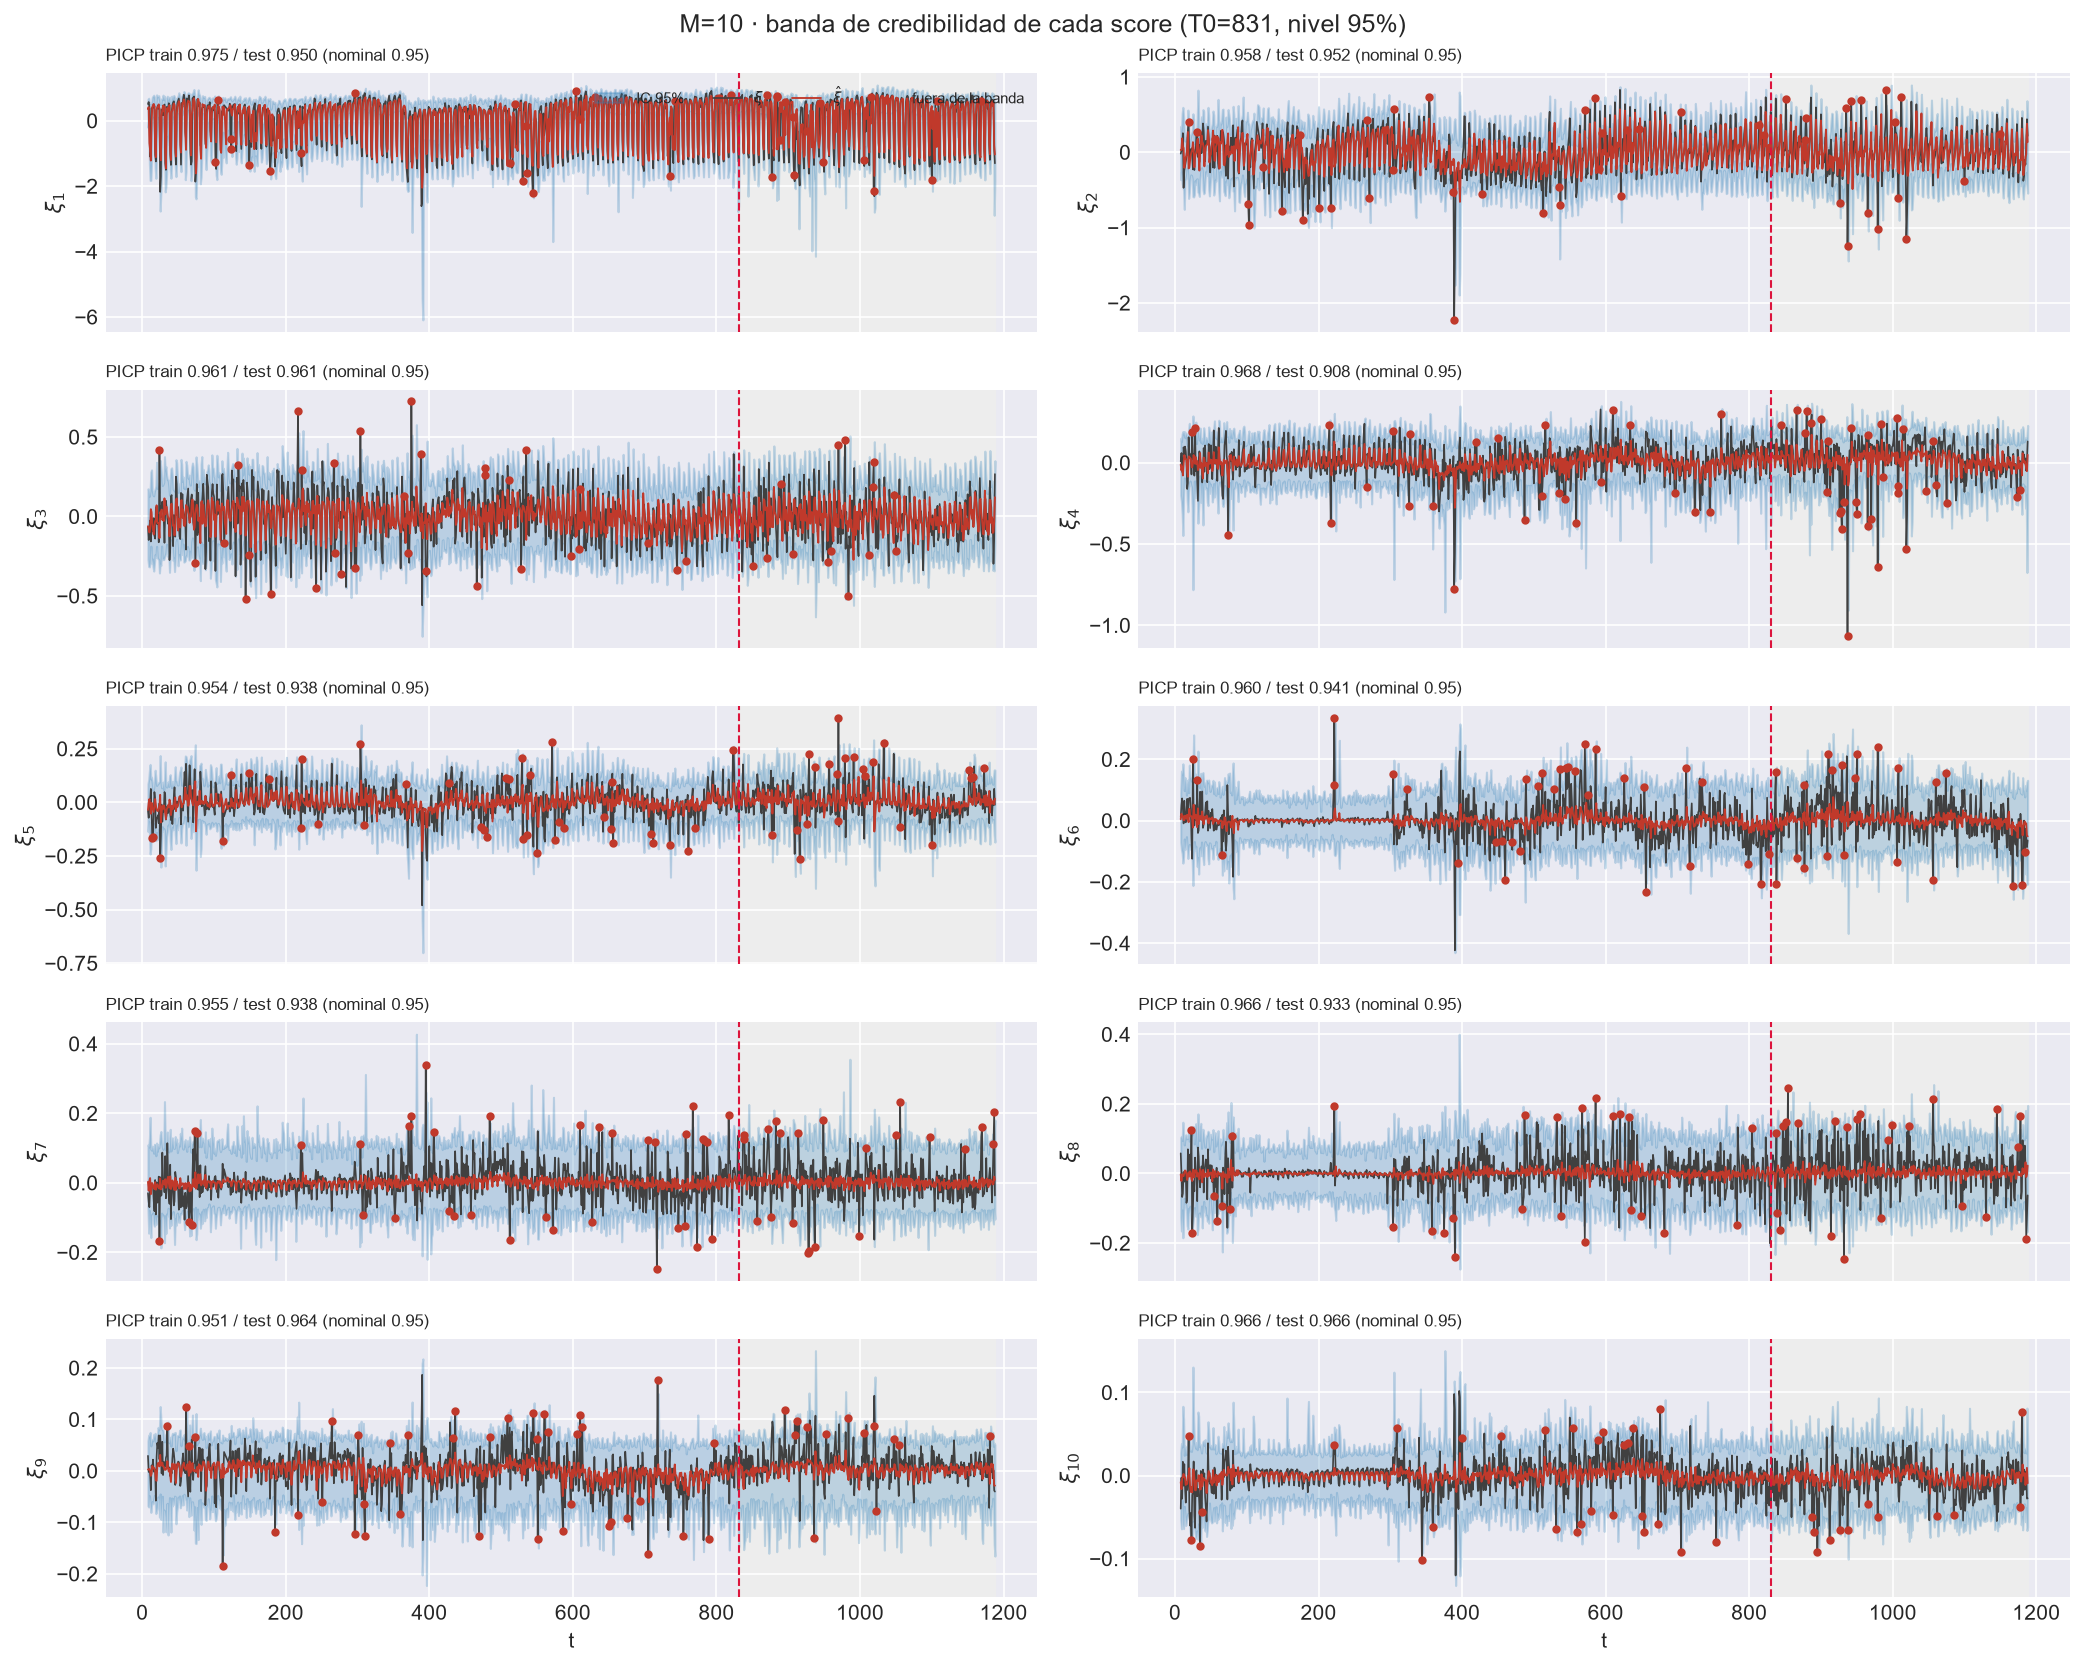
\includegraphics[width=\textwidth,height=0.75\textheight,keepaspectratio]{IMG/aneC_00/aneC_00_92_scores_banda_credibilidad_102.png}
\caption{Banda de credibilidad al 95\% de cada score, tráfico $\{1,7\}$ ($M = 10$).}
\label{fig:aneC_92_scores_banda_credibilidad_102}
\end{figure}

\begin{figure}[H]
\centering
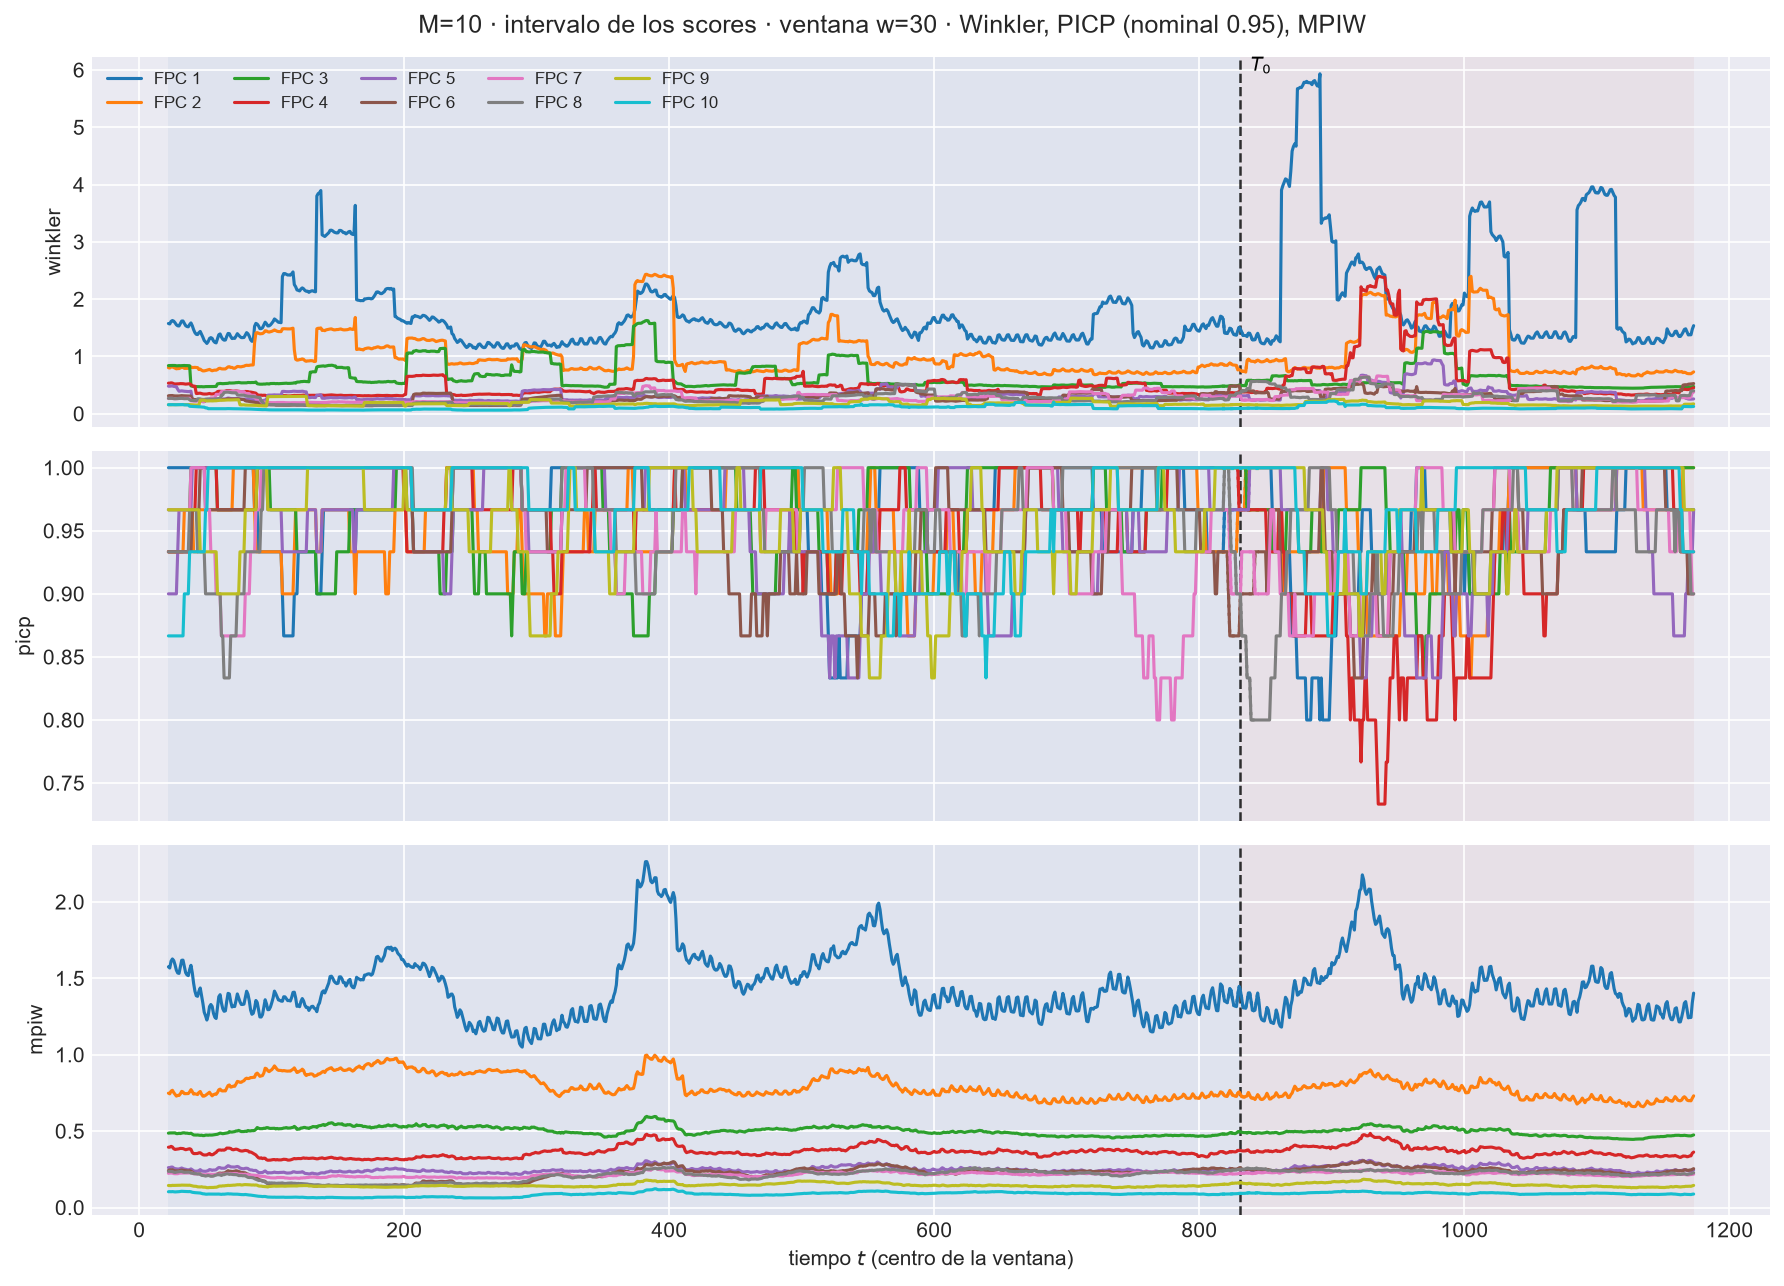
\includegraphics[width=\textwidth,height=0.75\textheight,keepaspectratio]{IMG/aneC_00/aneC_00_93_ventana_scores_intervalo_w30_102.png}
\caption{Métricas de intervalo de cada score sobre la ventana móvil, tráfico $\{1,7\}$ ($M = 10$).}
\label{fig:aneC_93_ventana_scores_intervalo_w30_102}
\end{figure}

\begin{figure}[H]
\centering
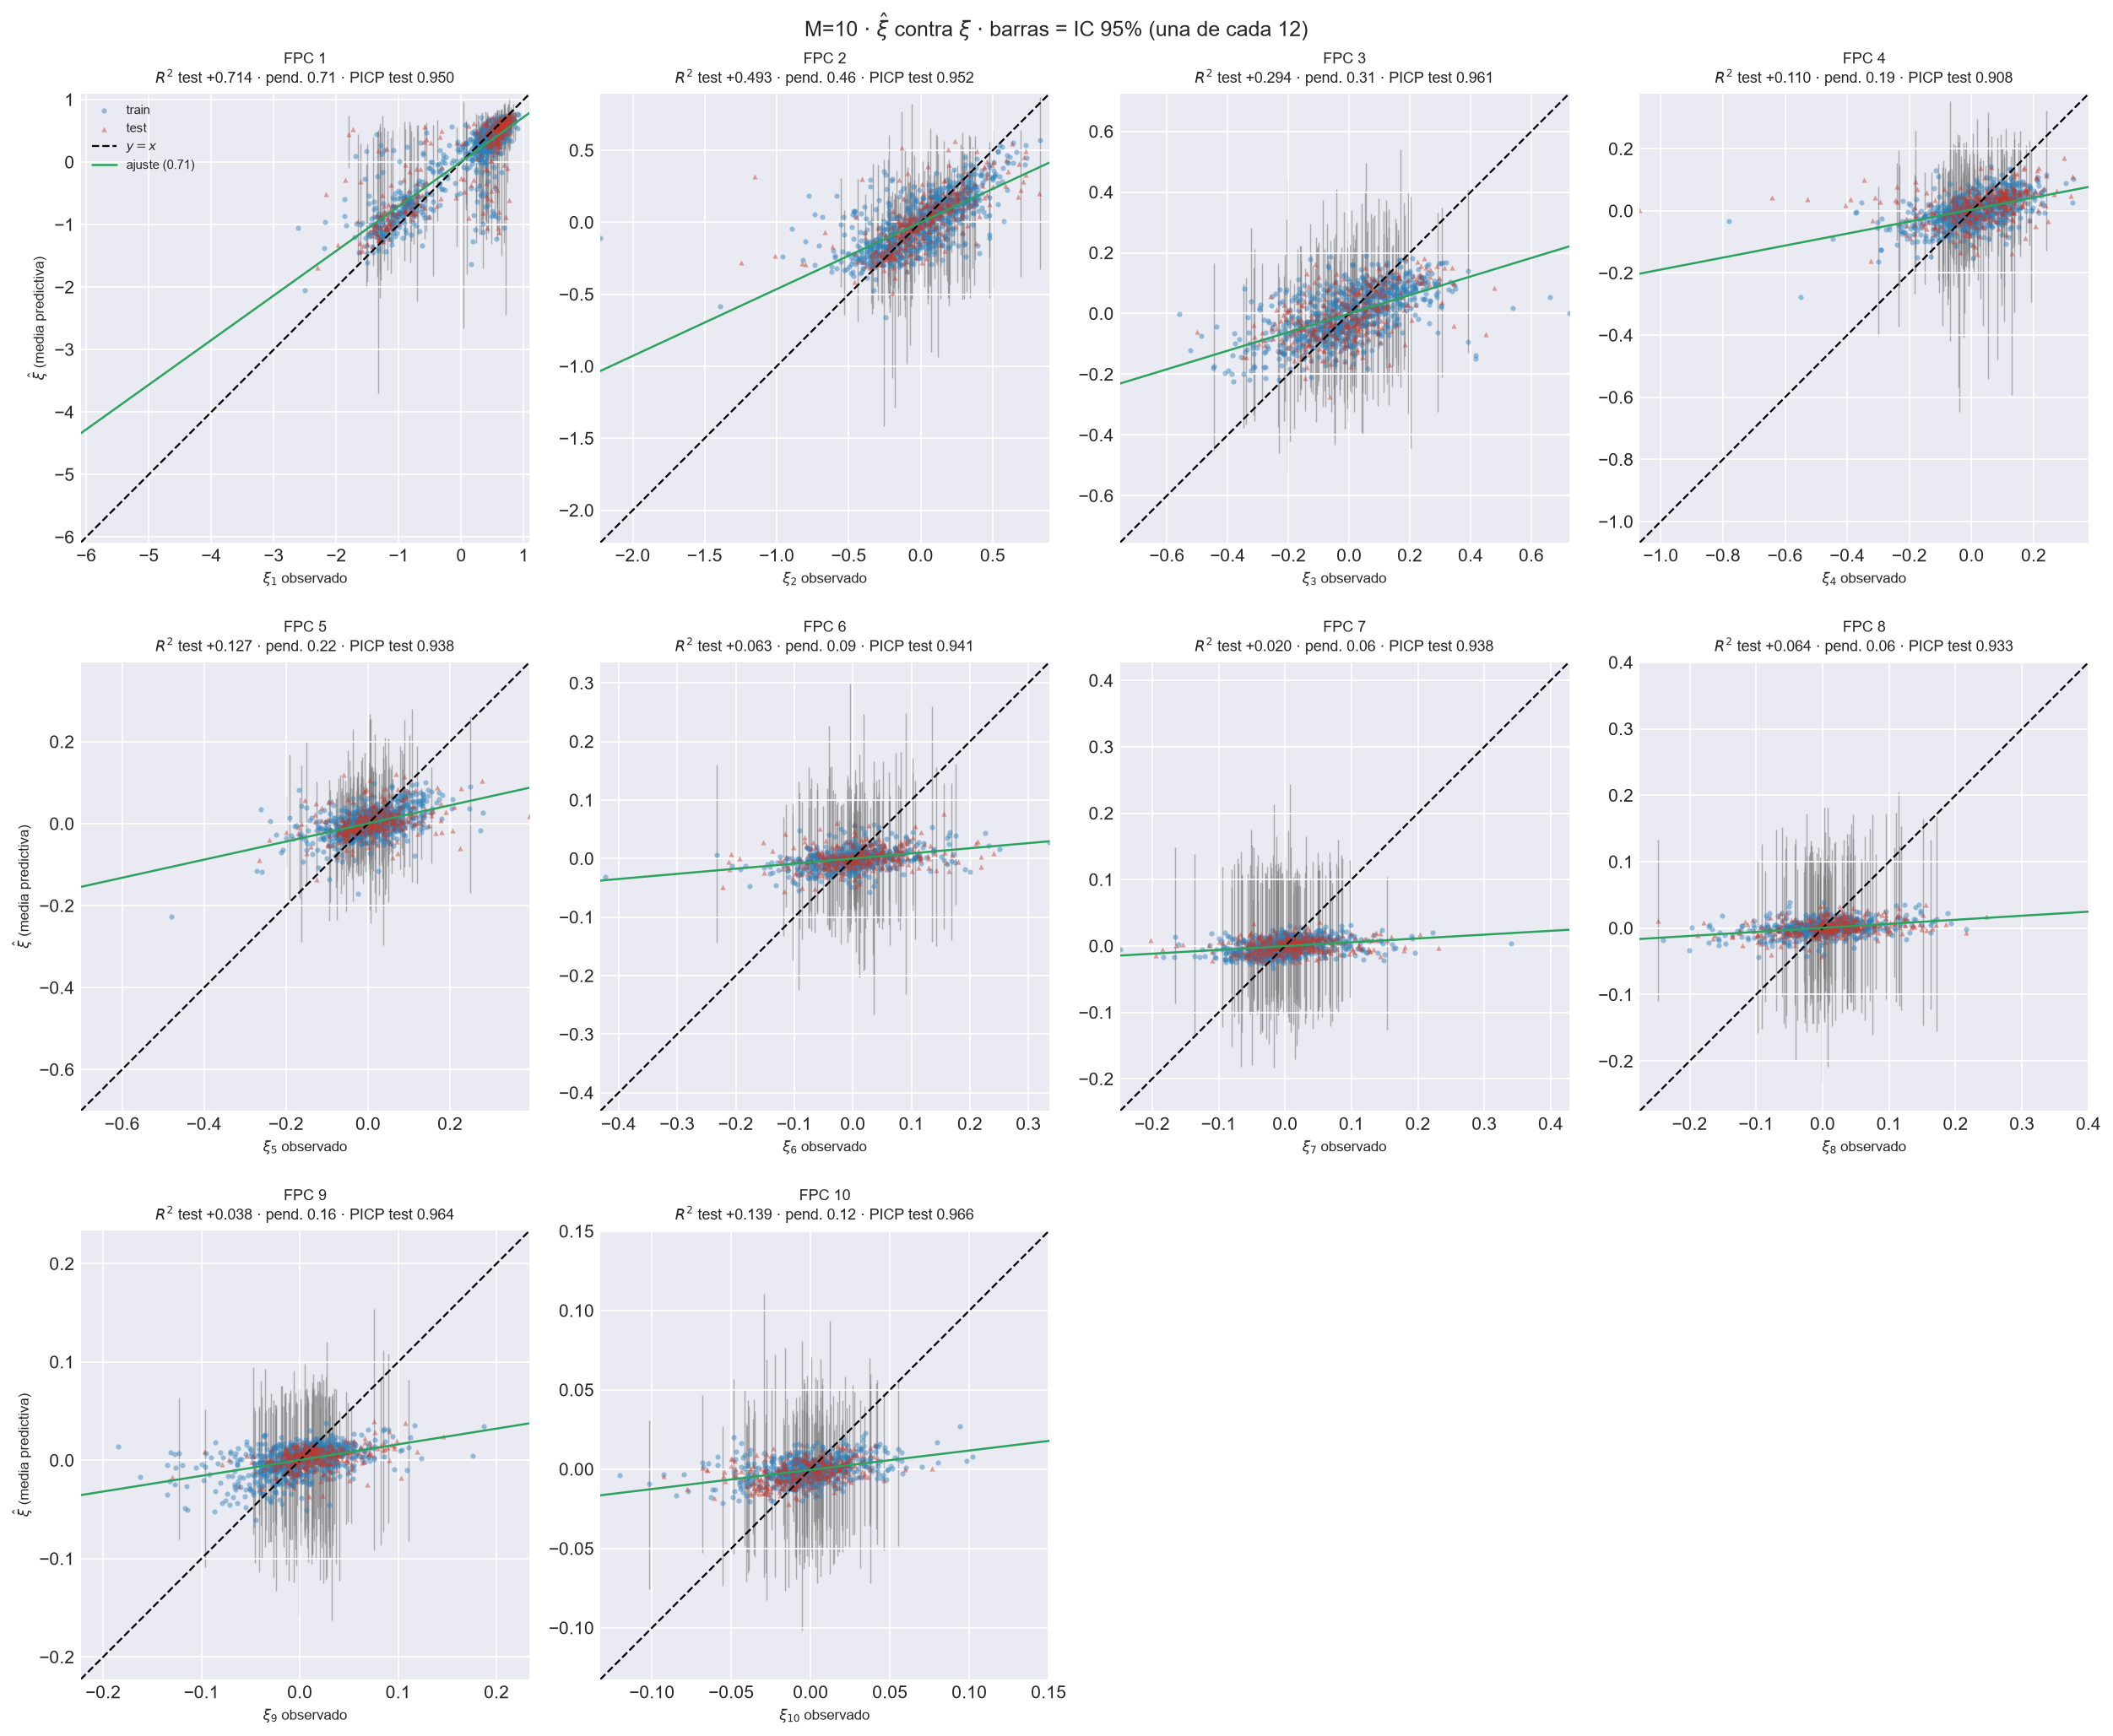
\includegraphics[width=\textwidth,height=0.75\textheight,keepaspectratio]{IMG/aneC_00/aneC_00_94_scores_dispersion_vs_real_102.png}
\caption{Dispersión estimada de cada score frente a la observada, tráfico $\{1,7\}$ ($M = 10$).}
\label{fig:aneC_94_scores_dispersion_vs_real_102}
\end{figure}

